\documentclass[12pt,letterpaper,oneside]{book}
\usepackage[utf8]{inputenc}
\usepackage[english]{babel}
\usepackage[T1]{fontenc}

% text
\usepackage{lmodern}
\usepackage{anysize} % margins
\usepackage{relsize} % resize text
\usepackage{microtype} 
\usepackage{fontsize}
\usepackage{minted} % code in text

% geometry 
\linespread{1.4}
\pagestyle{plain}
%\usepackage[left=3cm,top=3cm,right=3cm,bottom=3cm]{geometry}
\usepackage{geometry}
\usepackage{marginnote}
\usepackage{adjustbox}
\usepackage[width=.95\linewidth]{caption}

% math
\usepackage{amsfonts,amsmath,amssymb,amsthm} 

% graphics
\usepackage{graphicx} % \includegraphics
\usepackage{wrapfig} % in text figures
\usepackage{float} % allows [H] on floats

% references and bibliography
\usepackage{xcolor}
\definecolor{purple}{rgb}{0.2,0.0,0.4}
\usepackage[colorlinks=true,allcolors=purple]{hyperref}
	\providecommand*{\listingautorefname}{Listing}
\usepackage[semicolon,round,sort&compress]{natbib}
\usepackage{csquotes}
%\usepackage{chapterbib}

\usepackage{xcolor}
\definecolor{purple}{rgb}{0.2,0.0,0.4}
\usepackage[semicolon,round,sort&compress]{natbib}
\usepackage{csquotes}
%\usepackage{chapterbib}
\usepackage[colorlinks=true,allcolors=purple]{hyperref}
% taken from https://www.aanda.org/for-authors/latex-issues/references
\bibpunct{(}{)}{;}{a}{}{,} %% natbib format for A&A and ApJ
\usepackage{twoopt}
\makeatletter
\newcommandtwoopt{\citeads}[3][][]{\href{http://adsabs.harvard.edu/abs/#3}%
{\def\hyper@linkstart##1##2{}%
\let\hyper@linkend\@empty\citealp[#1][#2]{#3}}}
\newcommandtwoopt{\citepads}[3][][]{\href{http://adsabs.harvard.edu/abs/#3}%
{\def\hyper@linkstart##1##2{}%
\let\hyper@linkend\@empty\citep[#1][#2]{#3}}}
\newcommandtwoopt{\citetads}[3][][]{\href{http://adsabs.harvard.edu/abs/#3}%
{\def\hyper@linkstart##1##2{}%
\let\hyper@linkend\@empty\citet[#1][#2]{#3}}}
\newcommandtwoopt{\citeyearads}[3][][]%
{\href{http://adsabs.harvard.edu/abs/#3}
{\def\hyper@linkstart##1##2{}%
\let\hyper@linkend\@empty\citeyear[#1][#2]{#3}}}
\makeatother
% taken from aa.cls
\newcommand*\aap{A\&A}
\let\astap=\aap
\newcommand*\aapr{A\&A~Rev.}
\newcommand*\aaps{A\&AS}
\newcommand*\actaa{Acta Astron.}
\newcommand*\aj{AJ}
\newcommand*\ao{Appl.~Opt.}
\let\applopt\ao
\newcommand*\apj{ApJ}
\newcommand*\apjl{ApJ}
\let\apjlett\apjl
\newcommand*\apjs{ApJS}
\let\apjsupp\apjs
\newcommand*\aplett{Astrophys.~Lett.}
\newcommand*\apspr{Astrophys.~Space~Phys.~Res.}
\newcommand*\apss{Ap\&SS}
\newcommand*\araa{ARA\&A}
\newcommand*\azh{AZh}
\newcommand*\baas{BAAS}
\newcommand*\bac{Bull. astr. Inst. Czechosl.}
\newcommand*\bain{Bull.~Astron.~Inst.~Netherlands}
\newcommand*\caa{Chinese Astron. Astrophys.}
\newcommand*\cjaa{Chinese J. Astron. Astrophys.}
\newcommand*\fcp{Fund.~Cosmic~Phys.}
\newcommand*\gca{Geochim.~Cosmochim.~Acta}
\newcommand*\grl{Geophys.~Res.~Lett.}
\newcommand*\iaucirc{IAU~Circ.}
\newcommand*\icarus{Icarus}
\newcommand*\jcap{J. Cosmology Astropart. Phys.}
\newcommand*\jcp{J.~Chem.~Phys.}
\newcommand*\jgr{J.~Geophys.~Res.}
\newcommand*\jqsrt{J.~Quant.~Spectr.~Rad.~Transf.}
\newcommand*\jrasc{JRASC}
\newcommand*\jaavso{Journal of the American Association of Variable Star Observers}
\newcommand*\memras{MmRAS}
\newcommand*\memsai{Mem.~Soc.~Astron.~Italiana}
\newcommand*\mnras{MNRAS}
\newcommand*\na{New A}
\newcommand*\nar{New A Rev.}
\newcommand*\nat{Nature}
\newcommand*\nphysa{Nucl.~Phys.~A}
\newcommand*\pasa{PASA}
\newcommand*\pasj{PASJ}
\newcommand*\pasp{PASP}
\newcommand*\physrep{Phys.~Rep.}
\newcommand*\physscr{Phys.~Scr}
\newcommand*\planss{Planet.~Space~Sci.}
\newcommand*\pra{Phys.~Rev.~A}
\newcommand*\prb{Phys.~Rev.~B}
\newcommand*\prc{Phys.~Rev.~C}
\newcommand*\prd{Phys.~Rev.~D}
\newcommand*\pre{Phys.~Rev.~E}
\newcommand*\prl{Phys.~Rev.~Lett.}
\newcommand*\procspie{Proc.~SPIE}
\newcommand*\qjras{QJRAS}
\newcommand*\rmxaa{Rev. Mexicana Astron. Astrofis.}
\newcommand*\skytel{S\&T}
\newcommand*\solphys{Sol.~Phys.}
\newcommand*\sovast{Soviet~Ast.}
\newcommand*\ssr{Space~Sci.~Rev.}
\newcommand*\zap{ZAp}

% paragraph notes thing
\newif\ifvisibleintent

\newcommand{\intent}[1]{
	\ifvisibleintent
		\reversemarginpar\marginnote{\tiny #1}
	\fi
}











% TOC
\usepackage[titletoc]{appendix}

\begin{document}
	\begin{titlepage}
		\begin{center}
			
\includegraphics[width=10cm]{img/logo-uniandes.pdf}
			
			\vspace{2cm}
			
			{\fontsize{25}{40}\selectfont \bf The other spectrum of the stars\par}
			
			\vspace{10mm}
			
			{\huge Santiago Henao Castellanos}
			
			\vspace{10mm}
			
			{\huge Director: Dr. Alejandro García } 
			
			\vspace{15mm}
			
			{\large
				A thesis submitted in partial fulfillment\\
				for the degree of Bachelor of Physics
			}
			
			\vspace{5mm}
			
			{\Large
				Universidad de los Andes\\
				Science Faculty, Physics Department\\
				Bogotá, Colombia\\ \phantom{} \\
				December 6th, 2021
			}
		\end{center}
	\end{titlepage}

\frontmatter

\chapter*{Resumen}

La relación Período-Luminosidad para estrellas variables Cefeidas es una herramienta importante para medir distancias en la escala intergaláctica cercana.
Dado que las series de tiempo en astronomía terrestre están usualmente muestreadas de manera no uniforme, 
deben usarse técnicas alternativas al análisis de Fourier clásico para poder determinar el período de una estrella variable.

Por lo tanto aquí se presentan varios algoritmos para la exploración del espectro de Fourier de una señal arbitrariamente muestreada en el tiempo,
y se comparan unos con otros en términos de velocidad y robustez.
El mejor de ellos es usado para encontrar los períodos de las Cefeidas clásicas de las Nubes de Magallanes, usando los datos del proyecto OGLE-IV.
Con estos períodos y con el índice Wesenheit desenrojecido se reproducen las relaciones Período-Luminosidad para las Nubes de Magallanes.

\chapter*{Abstract}

The Period-Luminosity relation for Cepheid variable stars is an important tool to measure distances in the near intergalactic range. 
As time series in terrestrial astronomy are usually sampled in an uneven manner, 
alternative techniques to classical Fourier analysis must be used in order to determine the period of a variable star.

Therefore, several algorithms are presented that allow the exploration of the Fourier spectrum of a signal with arbitrary temporal sampling.
These algorithms are implemented and examined for speed and robustness. 
The best one is then used to find the periods of the classical Cepheids from the Magellanic Clouds, with data from the OGLE-IV project. 
Those periods and the Wesenheit extinction-free index are used to plot the Period-Luminosity relations for the Magellanic Clouds.


\newpage

\begin{flushright}
	\textit{
		I dedicate the prose to Trinidad,        \\
		for making the morning coffee            \\
		that fueled the writing of this document
	}

	\vspace{5mm}

	\textit{
		But all the code is for Miguel             \\
		who will not be able to compile it anymore \\ 
		but I think he would have liked it anyway.
	}
\end{flushright}

\vspace{2mm}

\chapter*{Acknowledgements}

There were a lot of people who provided me with their guidance and support on the process of writing this document. 
It was not purely a research process, but a personal voyage of discovery and motivation. 

Thus, I would like to thank first Alejandro García, the director of this monograph, 
for motivating me since the beginning of my career, and being patient with its eventual delay. 
The realization of that career would not have been possible without the gargantuan support and love of my parents and my family, 
who were there on every step along the way.
Neither without the aid of the University itself, which staff gave me and others%---and others--- 
the opportunity of continuing our studies on the still ongoing world situation.

I am also grateful with my dearest friends: Miguel, Juan David, Valeria, Camilo, Juanita and the two Nathalias. 
My time at Bogotá would have been very sorrowful if not for them. 
Also my dear David, who on recent times of crisis took care of me back in my hometown.

Finally, I write this couple of words to attempt to express the unmeasurable gratitude I have for Laura.

\mainmatter

\tableofcontents

\newpage

\listoffigures
\listoftables
\listoflistings

\newpage

\visibleintentfalse

\chapter{Introduction}
\intent{Ancient stellar variability}

It is undeniable that ancient civilizations looked to the night sky with great interest. 
Stars were considered innamobile and immutable, with the notable exceptions of planets and Nov\ae{}, respectively.
But periodic stellar variability was probably known since antiquity too.
For instance, egyptians knew the period of Algol three millenia ago \citep{Jetsu2013,Jetsu2015},
and the mythology of several cultures seems to have some references to the phenomenon \citep{Wilk1996}. 
On some cases, periodic variable stars were recorded as Nov\ae{} on some ancient sources \citep{HOPENGYOKE1962}.

\intent{Western rediscovery}

The rediscovery of stars having periodic changes on their brightness is accredited to Fabricius, 
who discovered Mira ($o$ Ceti) in 1596 \citep{Hoffleit1997}.
That discovery was in direct contradiction with the classical philosophical view of the Universe, as in \cite[book I, part 3]{aristotle}: 
\enquote{so far as our inherited records reach, no change appears to have taken place either in the whole scheme of the outermost heaven or in any of its proper parts}.
On the following centuries several other stars were marked as candidates for periodic variables.
Edward Pigott and his collaborator John Goodricke were verifying those candidates in 1784 \citep{Hoskin1979}. 
Famously, \cite{Pigott1785} observed $\eta$ Aquil\ae{} and confirmed its variability, 
while \cite{Goodricke1786} observed $\delta$ Cephei, Algol, $\beta$ Lyr\ae{}, and others.


\intent{Initial theories for stellar variablity}

Pigott and Goodricke results are remarkable, as almost a century would pass until the formalization of the magnitude scale for brightness by \cite{Pogson1856}.
But despite the lack truly (instrumental) quantitative measurments of brightness, 
there were plenty of theories regarding the mechanism behind variability. 
Those theories included planetary eclipses, star-star collisions, binary stars, meteor impacts, 
obfuscation by gas or dust clouds, and sun-like spots coupled with rotation and axial tilts \citep{Hoffleit1993}. 
And although the eclipse conjecture was later proved to be the correct for Algol \citep{Pickering1880}, 
the assymetric behaviour of the brightness of some stars (as those seen in Figure \ref{fig:first-cepheids}) could not be accounted for.
If the change of brightness were the product of an eclipse,
the star brightness would spend the same amount of time increasing as decreasing,
as the transiting object covers and uncovers the star.
On the same train of thought, if the star happened to have a side full of spots, or obscured by Nebul\ae{},
no stable rotation or movement could make the brightness go from minimum to maximum faster than from maximum to minimum on a periodic manner.

\begin{figure}[H] 
	\centering
	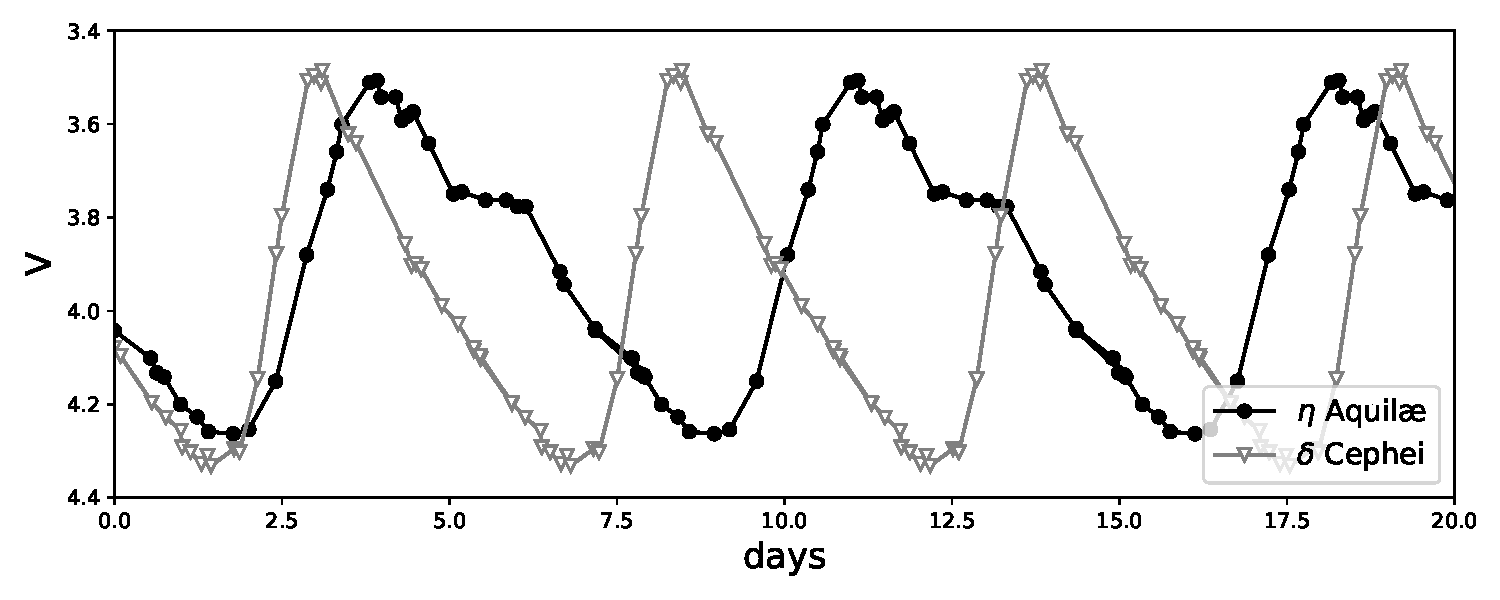
\includegraphics[width=0.9\textwidth]{img/eta_aquilae_delta_cephei_light_curves.pdf}
	\caption{Modern light curves for the first two discovered Cepheid variable stars. 
	$\eta$ Aquil\ae{} has a period of $\sim7.17$ days, in contrast with the $\sim5.36$ days of $\delta$ Cephei.
	Objects are brighter as magnitude (V) decreases (see chapter 2 for details). 
	Note how both stars take more time decreasing their brightness than increasing it. 
	Figure reconstructed from \cite{Kiss1998} data.}
	\label{fig:first-cepheids}
\end{figure}

\intent{Early classification}

These variable stars were initially classified by \cite{Pickering1880}, only taking into account the shape of the light curve: 
Nov\ae{}, Mira-like, eclipsing, irregular variables, and class for the aforementioned irregular (but highly periodic) case, namely $\beta$ Lyr\ae{} and $\delta$ Cephei.
There was a need for further classification of these stars, with several attempts of break down Pickering classes \citep{Lockyer1896,Lockyer1897}, 
but it would take several important discoveries in astronomy for the classification of variable stars to fully develop,
resulting in $\delta$ Cephei as the prototype of its own class of variable stars.
% log day units in caption

\intent{Work and discoveries of the Harvard Computers}

The next big steps on the field were done by Pickering's ``computers'' women at Harvard. 
Although the universities refused to let women study at the time, Pickering (then director of Harvard's observatory) needed people to process and analyze the sheer amount data in the observatory, 
on the form of stellar spectra and photographic plaques of the observations.
Working there, Williamina Fleming prepared the Draper Catalogue of stellar spectra \citep{Pickering1890}, 
which allowed her to classify Mira-type stars and Nov\ae{} with only their spectrum. 
This classification system was later reordered by \cite{Canon1901} to reflect the temperature of the stars.
Around that time Henrietta Leavitt joined the Harvard computers, 
with the task of searching for variable stars in the Magellanic Clouds, which at the time were classified as Nebul\ae{}.
There she discovered almost two thousand variables \citep{Leavitt1908}, the majority of which turned out to be of the $\delta$ Cephei class. 
By calculating the periods of 25 of those stars and comparing them to their maximum and minimum magnitudes, Leavitt found a linear relationship (Figure \ref{fig:leavitt}).

\begin{figure}[H] 
	\centering
	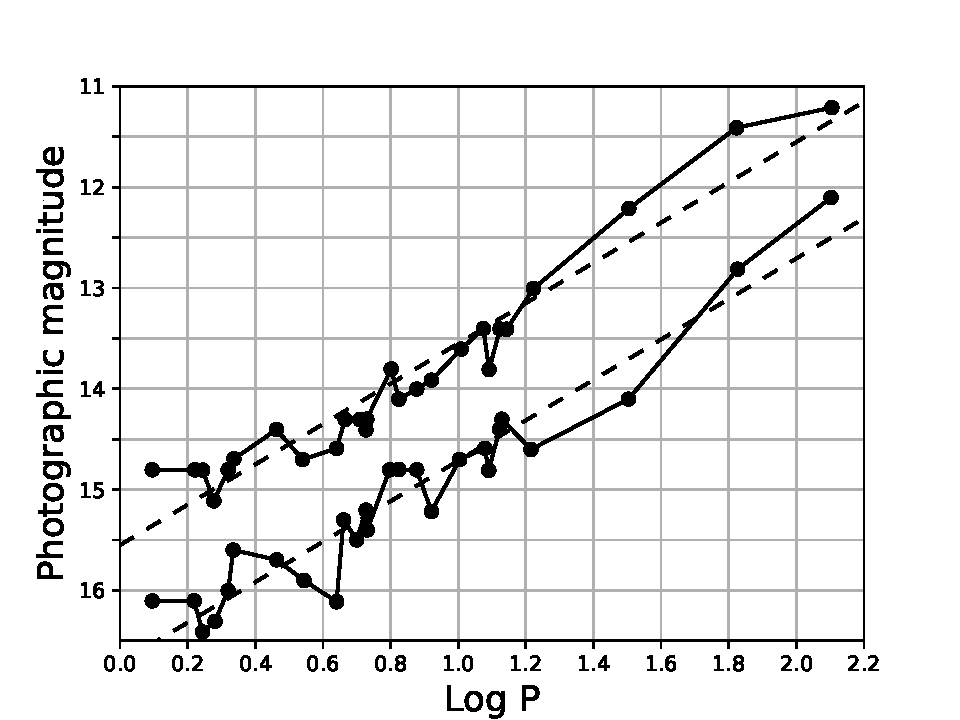
\includegraphics[width=0.7\textwidth]{img/leavitt.pdf}
	\caption{\cite{Leavitt1912} representation of the relationship between period and luminosity 
	of 25 Cepehid stars in the Small Magellanic Cloud.
	The two data series refeer to the points of maximum and minimum brightness for each star. 
	The period of the stars ($P$) is reported on days, so the abscissa is in units of $\log(\text{days})$.
	The ordenate is given in photographic magnitude.
	}
	\label{fig:leavitt}
\end{figure}

\intent{Period-Luminosity relation}

Leavitt's discovery was of immense importance as a possible tool for measuring the distance to the farthest cepheid stars. 
She noted: \enquote{Since the variables are probably at nearly the same distance from the Earth,
their periods are apparently associated with their actual emission of light} \citep[page 3]{Leavitt1912}.
Leavitt knew she was seeing the \textit{apparent} brightness of the stars, as brightness decreases with distance.
If distances to near cepeheids could be found by another method, 
this Period-Luminosity (PL) relation could be reversed to find the \textit{absolute} brightness of the Cepheids in the Small Magellanic Cloud (SMC),
finding the distance to the satellite galaxy (then called Nebul\ae{}).
Leavitt correctly proposed the method of parallaxes to solve this task, but his work on Harvard did not let her pursue this investigation.

\intent{fine-tuning the PR relation and the Magellanic clouds}

The parallaxes for the nearest Cepheids were examined by \citep{Hertzsprung1913}.
He used Leavitt's PL relation to calculate the distance to the SMC, 
giving ---after a \enquote{pen error} \citep{Fernie1969}--- 30~kilo-lightyears (kly), which is a vast underestimation.
\cite{Shapley1918} improved further the precision of Leavitt's original PL relation, 
but its zero point (its accuracy) was assumed to be the correct one, despite having several sistematic and selection errors \citep{Fernie1969}.
Shapley used his results to calculate the distance to the Magellanic Clouds, 
obtaining $106\pm5$ kly for the Small Cloud \citep{Shapley1924S} and $112\pm12$ kly for the Large Cloud \citep{Shapley1924L}.

\intent{The great debate, and Hubble measuring the size of the universe}

Around this time, there was a big debate in the astronomical community around the nature of the so-called \enquote{spiral nebul\ae{}}.
Were those nebul\ae{} part of the Milky Way, or were they their own separate, distant galaxies?
E. Hubble, using Shapley version of the PL relation, settled the matter when he found a distance of $\sim929$~kly for M31 and M33 
(now called the Andromeda and the Triangulum galaxies) and $\sim697$~kly for NGC 6822 (Barnard's galaxy) \citep{Hubble1925a,Hubble1925b}, 
surpassing Shapley's hypothesis that the galaxy was only 300 kly wide.

\intent{Space means time: the Cosmic age problem}

With this results, \cite{Hubble1929} measured the redshift of some extra-galactic Nebul\ae{}, 
and encountered a linear relationship between distance as velocity.
It was the first experimental evidence of the general relativity prediction of an expanding universe \citep{Fiedmann1922,Lemaitre1927}.
Hubble estimate of this expanding rate was $H_0 \approx 550 (\text{km}/\text{s})/\text{Mpc}$ (the Hubble constant), 
which implied the universe must have an age of $~2\times10^9$ years. 
Meanwhile, geologists estimated the age of the earth as $~4\times10^9$ years \citep[see][ for an historical account]{Dalrymple1994}.
How could be the Earth older than the universe? There was a big problem in the figures, somewhere.

\intent{Baade correction}

Hubble, again, had half the answer. He had some concerns about the zero point of Shapley's PL relation, 
an opinion shared with \cite{Baade1944} after he divided the stars on two populations based on their metallicities.
Baade realized that population I Cepheids were 1.5 magnitures brighter than population II (for the same period) 
so there were \textit{two} different PL relations, shifted on their zero point by 1.5 magnitudes.
He proved this hypothesis at Palomar Observatory, observing the Andromeda nebula \citep{Baade1956} \citep[see][for another discussion]{Arp1955}.
As a consequence of the distance-modulus equation, measurements made with population I Cepheids should be scaled by a factor of $10^{3/10}\approx 2$.
The Hubble distances were based on population I Cepheids, and  therefore his distances doubled, and consequently the observed age of the universe.
\cite{Patterson1955} measured the age of the Earth as $4.5\times10^9$ years, so the problem was not solved yet.

\intent{Sandage correction}

A second correction came from the work of Scandage. First reviewing Hubble's work with more data \citep{Sandage1956}, and then correcting a problem:
Hubble had made the calibration of the distance for the farthest nebul\ae{} with the brightest resolvable stars he had,
possible incurring in an identification mistakes with ionized Hydrogen regions or multiple nearby stars \citep{Sandage1958}.
This considerations amounted a total correction of 4.1 magnitudes, 
and produced a Hubble constant of $H_0 \approx 75 (\text{km}/\text{s})/\text{Mpc}$, 
or a timescale for the universe of $\sim1.3\times 10^{10}$ years, comparable to modern estimates \citep{Freedman2001}.

\intent{Present status of the distance ladder}

In the present day, mainly two astronomical projects are entitled to the search of variable stars and the refinement of cosmic distances estimation:
the OGLE project\footnote{\url{http://ogle.astrouw.edu.pl/}} and the Araucaria project\footnote{\url{https://araucaria.camk.edu.pl/}}.
While the Gaia space observatory measures parallaxes, the first step on the distance ladder, 
the OGLE project surveys the galaxy and the Magellanic Clouds in search of variable stars and gravitational microlensing.
They have nearly completed Leavitt initial task of catalogue the Cepheid stars on the Magellanic Clouds \citep{OGLE2017},
and their survey of Cepheids on the Milky Way has allowed to further study its structure \citep{Skowron2019} and its dynamics \citep{Mroz2019}.
On the other side, the Araucaria project focuses on the calibration of standard candles, comparing different methods: 
they have calibrated the distance to the SMC within a 3\% of precision \citep{Araucaria2014} and to the LMC within a 1\% \citep{Araucaria2019}.


\intent{The other spectrum, the Fourier spectrum}

Just one more particular problem has surfaced on the PL relation. 
As a consequence of the pulsation mechanism of these stars, 
the underlying physical machinery that makes their brightness oscillate,
Cepheid variable stars can pulsate on several \textit{overtones} of their natural frequency.
This overtones displaces the PL relation, as is multiplicative operation on the period, 
which amounts on a different position on the $\log P$ axis.
Therefore, stars with different modes of pulsation must be separated before attempting to calibrate a PL relation \citep{Zabolotski2005}.
The most natural way of attacking this problem is using the other spectrum of the star: 
not the light-energy usual spectrum, but the Fourier spectrum, 
which allow us to see the frecuencies and phase properties of the light curve.

We have seen that as experimental techniques evolve and become more precise, 
the theoretical aspects of the PL relation became increasingly important for the accurate determination of distances on the universe.
Even so, with the amount of observational data these projects are producing, 
the use of efficient and robust methods for analyzing it became imperative.

Although of capital importance, the methods of image reduction and magnitude determination lie outside the scope of this work.
The aim of this monograph is to examine and implement the different methods for finding the period of a Cepheid variable star.
Each method will be tested on real Cepheid data, in order to select the one better suited for the task of producing reliable PL relations.
The resulting method (or combination of methods) will be used to replicate the PL relations of the Cepheids on the Magellanic Clouds given by \cite{OGLE2016}.




	
\chapter{Theoretical Framework}
\section{Light curves}

The main concept present on the photometric analysis of variable stars is the light curve:
a diagram representing the \textbf{temporal} evolution of the star's \textbf{brightness}. 
Light curves are used to describe all types of variable stars, both periodic and non-periodic. 
In the case of periodic variable stars, a \textbf{phased} light curve is often preferred.

In order to properly study variable star, we need to have solid definitions for \enquote{temporal}, 
\enquote{brightness} and \enquote{phase} measurements.

\subsection{Julian Dates}
	
	\intent{Common calendars as a mixed-radix complicated unit}
	
	Calendars have existed for as long as humans have been able to keep track of time; since the dawn of astronomy.
	But similarly to the astronomical and physical sciences, calendars change with culture and also with time itself.
	The daylight, lunar and seasonal cycles do not align nicely; their periods are not a simple fraction of each others.
	This causes all calendars that try to align the day period with any other solar system based period to be a mixed radix unit full of exceptions.
	If your calendar is moon-based, your months will have unequal number of days.
	If your calendar is season-based, your years will have unequal number of days.
	Either way, computing day differences will be a nightmare. 
	You cannot have an integer calendar without leap days every few years.
	
	\intent{Troubled days}
	
	So, the only option is to do neither and just count the number of days. 
	But as discussed before, the year to day ratio is far from a simple fraction;
	by the time the earth makes a full revolution around the sun (with respect to the other stars),	a non-integer number of days have passed.
	But this seems fine, then. If you accept to deal with decimals, you can just take your base unit as a solar day, noon to noon,
	easy enough to measure and compare.
	
	\intent{Atomic clocks confidence}
	
	Except, the solar day is not exactly constant. The time from terrestrial noon to noon is not a constant number of seconds \citep{McCarthy1986}.
	Now what, measure everything in seconds? will the same argument hold here, and the second will turn out to be variable? 
	It turns out we have a very constant, precise definition for a second. 
	According to the 2019 redefinition of the International System of Units (SI),
	one second is exactly \citep{si-brochure}:
	\begin{equation}
		1\text{ s} = \frac{9\,192\,631\,770}{\Delta\nu_{\text{Cs}}} \label{eq:SI-second}
	\end{equation}
	Where $\Delta\nu_{Cs}$ is the unperturbed ground-state hyperfine transition frequency of ${}^{133}\text{Cs}$, which is a fundamental physical constant.
	Then, supported by hundreds of years of experiments in the natural sciences, we measure everything in seconds. 
	
	\intent{The Unix Time and the Julian Date}
	
	%A commonly used time unit based on this definition is the (TAI-based) Unix Time: 
	%the number of seconds since January 1st 1970, without leaps \citep[XRAT A.4.16]{POSIX2017}.	
	But for astronomical events, seconds are a tiny unit. Measuring temporal scales of days and years in seconds is cumbersome and unpopular.
	Besides, historical astronomical records ---even Before the Common Era--- were and are still in use \citep{Morrison2004},
	and astronomers and historians liked to have a unit of time that did not extend to the negative numbers.
	Therefore astronomical dates were historically to be measured in days since a date early enough to capture historical records.
	The original idea for this zero point came from Joseph Scaliger in 1583 \citep{Carroll2017}. 
	He considered three time periods used in his day:
	
	\begin{itemize}
		\item The solar cycle: in the Julian calendar, the weekday of a given date on the year would repeat every 28 years 
			\footnote{With exactly $365.25 = 1461/4$ days in a year and 7 days a week, the week days cycle every $\text{LCM}(1461,7)=10227$ days, $=28$ years.}. 
			The solar number of a (Julian) calendar year $y$ in this cycle is given by
			\begin{equation}
				\text{SolarNumber}(y) = \text{mod}(y+8,28) + 1
			\end{equation}
			
		\item The lunar cycle: 19 years, the number of years in which a moon phase will occur in the same day of the year
			\footnote{A mean synodic month (time between two full moons) is 29.53059 days. 235 synodic months was sufficiently close to 19 years for the Julian calendar.}.
			The so called \enquote{Golden Number} of a Julian year $y$ is given by 
			\begin{equation}
				\text{GoldenNumber}(y) = \text{mod}(y,19)+ 1
			\end{equation}
			
		\item the Indiction: a 15 year period for tax census used by the Roman Empire and later by the Holy Roman Empire. Its calculation for a Julian year is:
			\begin{equation}
				\text{Indiction}(y) = \text{mod}(y+2,15) + 1
			\end{equation}
	\end{itemize}
	
	The phases on the modulus operations are selected such that historical records make sense. The solution, then to the integer equation 
	\begin{equation}
		\text{SolarNumber}(y) = \text{GoldenNumber}(y) = \text{Indiction}(y) = 1
	\end{equation}
	is, using the Chinese remainder theorem,
	\begin{equation}
		y = 3268 + 7980 n
	\end{equation}
	were $n$ is any whole number. Scaliger selected $n=-1$ as the zero point for the Julian Day system, which would be Julian year $-4712$ CE, 
	and as there was no year 0, that would be Julian $4713$ BCE, or in the Gregorian modern calendar, noon of November 24, 4714 BCE (Epoch).
	
	\intent{Final definition and the R\o{}mer Delay}
	
	Those are the ingredients needed to define the modern Julian Day system. If an Ephemeris Day is defined as $24\times60\times60=86400$ SI seconds, 
	the Julian Day (JD) is the fractional number of Ephemeris days that have passed since noon of November 24, 4714 BCE on the current calendar. 
	There are at least 4 principal corrections to the Julian Day due to astronomical, geological or relativistic effects \citep{Eastman2010}, 
	but here we will only consider one of them, as it's the only strictly needed to understand the data used on this work.
	As earth moves around the sun, the light from a distant object may reach its surface with different time delays, consequence of the finite speed of light.
	In order to be able to accurately compare time series taken around all positions of earths orbit, 
	the signal is corrected with a delay as if the measurement was taken on the position of the sun.
	This is called \textbf{Heliocentric Julian Day} (HJD), and that correction is given by (see \autoref{fig:romer-delay}):
	\begin{equation}
		\Delta t = \frac{\vec{r}\cdot \hat{n}}{c} = - \frac{r}{c} \left(\cos\delta \cos \delta_{\odot}\cos(\alpha-\alpha_\odot)+ \sin\delta \sin \delta_\odot\right)
	\end{equation}
	where $\vec{r}$ is the vector sun-to-earth, $\hat{n}$ is the direction of the measurement on earth's sky, 
	and $(\alpha,\delta),\,(\alpha_\odot,\delta_\odot)$ are the equatorial coordinates of the observed object and the sun respectively, 
	as seen from earth, \textit{i.e.} $\vec{r} = (r,\phi=\frac\pi2-\delta_\odot,\theta=\alpha_\odot)$, $\hat n = (1,\phi=\frac\pi2-\delta,\alpha)$ 
	The maximum possible value for this correction is $\sim 1 \text{ AU}/c = 16.63 \text{ min } = 0.00577$ Ephemeris days.
	
	
	
	
	\subsubsection{Remark about floating point representations}
	
	\intent{Unit in last place of floating point data}
	
	Typically, decimal numbers are stored on a computer as a double-precision floating point number, 
	which is basically \enquote{fixed point} scientific notation in base 2, with 52 binary digits for the mantissa and 11 for the exponent \citep{IEEE2019}.
	Floating point numbers are of course imprecise, and in fact more as the number they represent grows. 
	To quantify this loss of precision exists the notion of the machine epsilon: 
	the difference from a given number to the next representable number on the system.
	This epsilon (also called \enquote{unit in last place}) is greater for greater numbers,
	and there is the question of whether we will lose or not our anhelated temporal scale precision.
	
	\intent{typical precision of the numbers used}
	
	As a random example from the OGLE IV database (see \autoref{sec:data}), let's check the precision at $\text{HJD}=2455262.5065$. 
	In \autoref{lst:c-eps} there is a simple function to estimate the precision. 
	If we use it with our number we'll get $\sim 4.6\times 10^{-10}$ days, which is $40 \,\mu \text{s}$. 
	If instead of the HJD we choose to store the number of seconds since the Julian Epoch ($\sim 2.12\times 10^{11} \,\text{s}$) 
	the precision would be $\sim 30 \,\mu \text{s}$.
	But this HJD in particular was stored as a \textit{reduced} HJD. In this case, the reported number was $\text{RHJD}=\text{HJD}-2.45\times 10^6 = 5262.5065$.
	The machine precision at $5262.5065$ is $\sim 9.09\times 10^{-13} $ days, or $78.5 \,\text{ns}$, 
	so we conclude that floating point precision is not a problem for the storage of this reduced time unit in this case.
	
\subsection{Magnitudes}

	\begin{figure}[H]
		\centering
		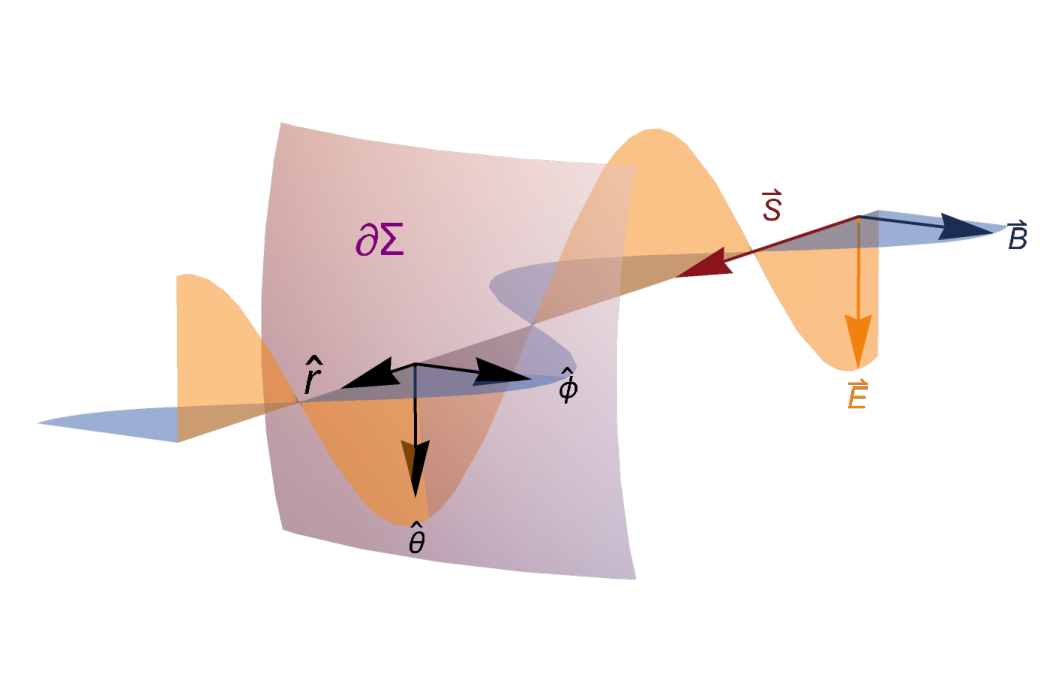
\includegraphics[width=0.6\textwidth]{img/Spherical_EM.pdf}
		\caption[Electromagnetic wave propagation through a spherical surface]{
			An electromagnetic wave ($\vec E,\vec B$) propagating outwards ($\vec S$) through a spherical surface $\partial \Sigma$ in a vacuum space.
			The correspondence of the directions of $\vec S,\vec B$ and $\vec E$ with the spherical directions $\hat r,\hat \phi, \hat \theta$ is to be noted.
		}
		\label{fig:spherical-em}
	\end{figure}
	
	\subsubsection{Energy conservation and the inverse square law}

	The magnitude system, vertical axis of a light curve, can be understood from the principles of electromagnetic waves.
	We would first want to ascertain the distance dependence of the energy flux for an isotropic light source.
	Here, isotropic means that the magnitude of the electric and magnetic fields of the wave would not depend on any angle.
	In spherical coordinates, for an outgoing wave of frequency $\omega$ and wave number $k$, we have (see \autoref{fig:spherical-em})
	\begin{equation}
		\vec E = E(r) \cos(kr-\omega t) \hat\theta \qquad \vec B = B(r) \cos(kr-\omega t) \hat\phi
	\end{equation}
	where $B(r)=E(r)/c$. Using Poynting's theorem \citep[\S8.1.2]{Griffiths2013} we can calculate the total energy flux\footnote{All the \enquote{energy fluxes} referred in this section are per unit of time.} through an entire sphere centered at the source.
	Fist, we calculate the Poynting vector 
	\begin{equation}
		\vec S = \frac{\vec E \times \vec B}{\mu_0} = \frac{\cos^2(kr-\omega t)E(r)^2}{c\mu_0} \,\hat r
	\end{equation}
	and its temporal mean 
	\begin{equation}
		\left<\vec S \right> = \frac{\omega}{2\pi}\int_0^{2\pi/\omega} \frac{\cos^2(kr-\omega t)E(r)^2}{c\mu_0} \,\hat r\;dt = \frac{E(r)^2}{2c\mu_0}\,\hat r \label{eq:poynting}
	\end{equation}

	Its flux is then the energy density flux through the whole spherical surface $\Sigma$ of radius $r$, also called Luminosity
	\begin{equation}
		L = \oint_{\partial\Sigma} \left<\vec S\right> \cdot d\vec{A} 
			= \oint_{\partial\Sigma} \left<\vec S\right> \cdot \hat r \; r^2 d\Omega
			= \oint_{\partial\Sigma} \frac{E(r)^2 r^2}{2c\mu_0} d\Omega
			= \frac{2\pi r^2  E(r)^2}{c\mu_0} \label{eq:luminosity}
	\end{equation}

	But the luminosity should \textit{not} be a function of the radius. 
	The electromagnetic energy that passes through a $r_0$-radius sphere should be the same that later passes through a $2r_0$-radius sphere.
	It's the same electromagnetic wave after all; there are no charges or currents. 
	Therefore, the magnitude of the electric field $E(r)$ should be inversely proportional to $r$, and that way $L$ is constant and energy is conserved.
	
	Knowing $E(r)$ we can then do the same process the other way around: 
	calculate the energy flux through a properly aligned detector of known area $A$,
	simply known as Flux	
	\begin{equation}
		F = \int_{S} \left<\vec S\right> \cdot \hat r \; dA = \frac{E(r)^2 A}{2 c \mu_0}
	\end{equation}
	where the integration occurs along the surface $S$ of the detector, which typically would be flat surface, 
	but considered here as a section of a sphere with a radius so immense that the difference is meaningless.
	As $E(r)\propto 1/r$, $F\propto 1/r^2$,  or equivalently, 
	\begin{equation}
		F(r)=\frac{L A}{4\pi r^2} \label{eq:flux}
	\end{equation}
	
	\subsubsection{Logarithmic scales}
	
	Working with the same example as before, if we put our detector at a distance $r=r_0$ of a source of light $a$,
	and measure a flux $F_a(r_0)$,
	the flux at a distance $2r_0$ will be $F_a(r_0)/4$, according to \autoref{eq:flux}. 
	In general, if we change the distance by a factor $d$, the change in flux would be $1/d^2$.
	
	But what if we wanted a brightness scale where \textit{multiplicative} changes on the distance became \textit{additive} changes of brightness?
	If we are confident in our measurement of $F_a(r_0)$, we could measure the fluxes relative to $F_a(r_0)$, 
	and define a new logarithmic unit for the brightness of any object $b$ as
	\begin{equation}
		\mathcal{F}_b(r) = \alpha \ln\left(\frac{F_b(r)}{F_a(r_0)}\right) \label{eq:general-magnitude}
	\end{equation}
	where $\alpha$ is a free parameter of our unit system. 
	That way, the \enquote{brightness} difference between a measure of object $b$ at distances $r_1$ and $r_2$ would be
	\begin{equation}
		\Delta \mathcal{F}_b = \mathcal{F}_b(r_2) - \mathcal{F}_b(r_1) 
			= \alpha \ln\left(\frac{F_b(r_2)}{F_b(r_1)}\right)
			= -2\alpha \ln\left(\frac{r_2}{r_1}\right)
			\label{eq:general-distance-modulus}
	\end{equation}
	where we used \autoref{eq:flux} as before. 
	One immediate consequence of this definition of brightness is that the brightness of the reference object $a$ at distance $r_0$ would be exactly 0.
	
	For our $\mathcal{F}$ to become the standard magnitude system, we have to choose $\alpha$, and $F_a(r_0)$
	
	\subsubsection{Historical choice for $\alpha$}
	
	In order to formalize the magnitude scale, and still maintain some sense with the historical records, 
	\cite{Pogson1856} proposed that an increment of 5 magnitudes would correspond to a flux 100 times \textit{smaller}. 
	That means that a magnitude 5 object would have a flux $F_b = F_a(r_0)/100$. 
	Replacing that in \autoref{eq:general-magnitude} and solving for $\alpha$ results in
	$$
		5 = \alpha \ln\frac{1}{100} \qquad \Rightarrow \qquad \alpha = \alpha = -\frac{5}{\ln 100} = -\frac{5}{\log_{10}(100)\ln(10)} = -\frac{2.5}{\ln 10}
	$$
	which allows us to rewrite \autoref{eq:general-magnitude} as 
	\begin{equation}
		\mathcal{M}_b(r) = -2.5 \log_{10}\left(\frac{F_b(r)}{F_a(r_0)}\right) \label{eq:magnitude}
	\end{equation}
	and \autoref{eq:general-distance-modulus} as
	\begin{equation}
		\Delta\mathcal{M}_b = \mathcal{M}_b(r_2) - \mathcal{M}_b(r_1) 
			= -2.5\log_{10}\left(\frac{F_b(r_2)}{F_b(r_1)}\right) 
			=  5 \log_{10}\left(\frac{r_2}{r_1}\right)
		\label{eq:magnitude-delta}
	\end{equation}
	which implies that a positive difference in magnitude of $1$ corresponds to a flux ratio $f$ of
	$$
		1 = -2.5 \log_{10}(f) \qquad \Rightarrow \qquad f = 10^{-1/2.5} = 0.3981
	$$
	and correspondingly, a negative difference in one magnitude corresponds to $10^{1/2.5}=2.51188$ times the flux.
	
	As is standard in astronomy, the 10 in $\log_10$ would be obviated from now on.
	
	\subsubsection{The reference flux, absolute and apparent magnitudes}
	
	The standard flux for the magnitude is defined by the International Astronomical Union as
	$F_a(r_0)=F_0= 2.518 021 002 \times 10^{-8}\text{ W}/\text{m}^2$ at $r_0=10\text{pc}$\;\footnote{A parsec is defined as $\text{pc}=648 000/\pi \text{AU}$}, 
	which corresponds to a luminosity $L_0=3.0128\times 10^{28} \text{ W}$ \citep[IAU, B2]{IAUB22015}. 
	
	With the reference flux, we can measure the flux of any light source and calculate its \textbf{apparent magnitude} $m$,
	which for an object $b$ is at a distance $r_b$ is defined using \autoref{eq:magnitude} as
	\begin{equation}
		m = -2.5 \log\left(\frac{F_b(r_b)}{F_0}\right)
	\end{equation}
	By the convention $r_0=10\text{ pc}$ the \textbf{absolute magnitude} is defined as
	\begin{equation}
		M = -2.5 \log\left(\frac{F_b(10\text{ pc})}{F_0}\right)
	\end{equation}
	If you know the distance $r_b$ and the apparent magnitude, you can calculate the absolute magnitude using \autoref{eq:magnitude-delta}:
	\begin{equation}
		m-M = 5 \log\left(\frac{r_b}{10 \text{ pc}}\right) \label{eq:distance-modulus}
	\end{equation}
	which is known as the distance modulus.
	
	Before the standard flux was given in base SI units, it was taken as that of Vega ($\alpha$ Lyr\ae{}).
	
	\subsubsection{Wavelength dependence on the magnitude}
	
	Until now there have been no discussion about the wavelength of the light on the energy flux. 
	But of course the energy of an electromagnetic wave depends on its wavelength. 
	For a black body, this is governed by the Planck's Law \citep{Planck1901}, stating that the spectral radiance
	\begin{equation}
		B_\lambda(T) = \frac{2hc^2}{\lambda^5}\left(e^{\frac{hc}{\lambda k_B T}}-1\right)^{-1}
	\end{equation}
	This spectral radiance is conceptually equivalent to the term $\left<\vec S\right>\cdot \hat r$ used in \autoref{eq:poynting} \footnote{
		The spectral radiance $B_\lambda$ is defined as the energy flux per hertz per second,
		and is in fact connected with the statistics of the magnitude of the electric field $E(r)$ considered before, 
		because the different occupation levels of some energies that arise from  the thermodinamical considerations.
		Again, refer to the original work of \cite{Planck1901}  for details.
	}. 
	With this approximation and with \autoref{eq:luminosity} we can define the monochromatic Flux and Luminosity \citep[Chapter~3, Section~5]{Carroll2017}:
	\begin{equation}
		F_\lambda \;d\lambda = \frac{L_\lambda A}{4\pi r^2} \;d\lambda = B_\lambda\left(\frac{R}{r}\right)^2 \;d\lambda
	\end{equation}
	where $R$ is the radius of the black body (the emitting sphere) and $r$ is the distance where the flux is measured.
	One can integrate that to obtain the Stephan-Boltzmann law:
	\begin{equation}
		L = 4\pi R^2 \sigma T^4
	\end{equation}
	With this equation we can deduce a way to calculate $F_{0\lambda}$, the standard flux at any given wavelength; 
	we have the standard luminosity: $L_0=3.0128\times10^{28}\text{ W}$, 
	and the Stefan-Boltzmann constant is $\sigma=5.6703744\times10^{-8}\frac{\text{W}}{\text{m}^2\text{K}^4}$. 
	Additionally, as the standard had to be numerically based on the previous standard, the emitting radius must be the radius of Vega \citep{Yoon2010}, $R\approx 1.789 \times 10^9 \text{m}$.
	From that we deduce an effective temperature $T_0 = 10720 \text{ K}$
	
	\subsubsection{The Johnson-Cousins photometric system}
	
	Albeit one \textit{could} study starlight in a monochromatic fashion, 
	it would be instrumentally and phenomenologically inconvenient to work with individual wavelengths.
	Rather, astronomers use filters to focus their attention on a portion of the spectrum,
	usually based on the spectral properties of the target object or star.
	
	Each filter is an optical device that let the light pass through more or less depending of its wavelength.
	This function is called the transmittance of the filter. 
	
	The most commonly used photometric system of filters is called the Johnson-Cousins UBVRI system. 
	Transmittance curves for these five filters, one for each letter, are given in \autoref{fig:filters},
	along with the filters used in the OGLE-IV project. 
	But in place of a full function, it is common to give an effective wavelength and bandwidth for the filter. 
	This is presented on \autoref{tab:filters}.
	
	\begin{figure}[H]
		\centering
		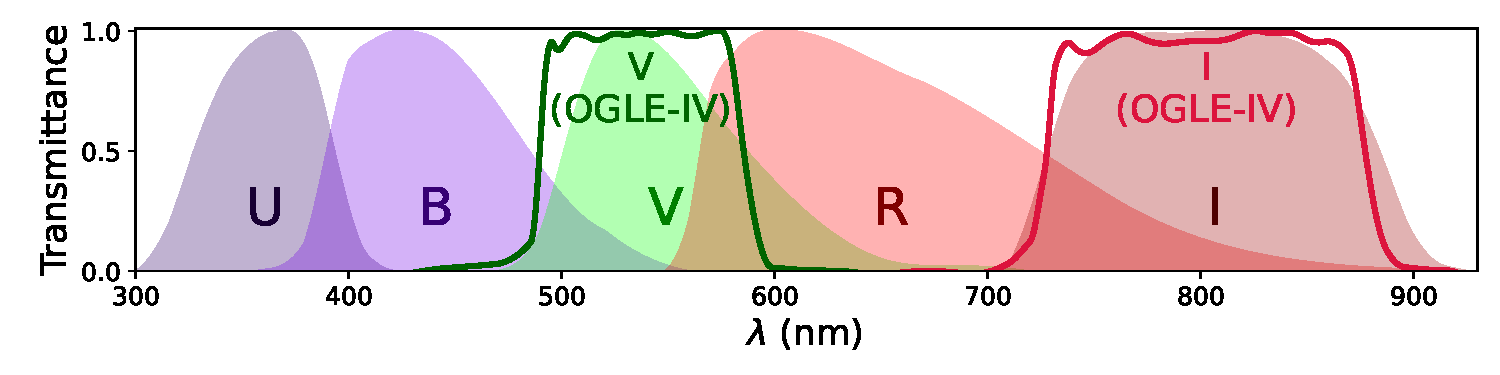
\includegraphics[width=\textwidth]{img/filters.pdf}
		\caption[Johnson-Cousins and OGLE-IV photometric systems]{
			Johnson-Cousins (filled) and OGLE-IV equivalent (solid) filters transmittance curves. 
			Colors are meant to be representative, not exact. UBVRI curves were adapted from \cite{Bessell2005}, and OGLE-IV curves from \cite{OGLE2015}. 
			It is to note that OGLE-IV curves are experimental measurements of custom made filters.
		}
		\label{fig:filters}
	\end{figure}
	
	\begin{table}
		\centering
		\begin{tabular}{c|c||c|c}
			Filter & description & $\lambda_{eff}$ (nm) & $\Delta_{\lambda}$ (nm) \\ \hline\hline
			U & Ultraviolet & 366.3 & 65 \\ 
			B & Blue & 436.1 & 89 \\ 
			V & Visual & 544.8 & 84 \\ 
			R & Red & 640.7 & 158 \\ 
			I & Infrared & 798 & 154
		\end{tabular}
		\caption[Johnson-Cousins effective wavelengths and bandwidths]{
			Effective wavelengths and bandwidths for the Johnson-Cousins photometric system. Data from \cite{Bessell2005}.
			}
		\label{tab:filters}
	\end{table}
	
	Absolute magnitudes for an object in these standard filters are presented as a sub-index: $M_B$ would be the blue absolute magnitude.
	Relative magnitudes are presented as the filter letters: $B$ would be the blue apparent magnitude.
	
	If the transmittance function of a filter \enquote{X} is denoted $T_X(\lambda)$, the apparent magnitude $X$ is physically obtained by the process
	
	\begin{equation}
		X = \int_0^\infty T_X(\lambda) R(\lambda) F(\lambda) \,d\lambda
	\end{equation}
	
	where $F(\lambda)$ would be the monochromatic flux (the light spectrum) of the star, 
	and $R(\lambda)$ would be the optical response of the instrumental system used to take the measure, without the filter
	\footnote{this would include things like the optical response of the telescope and mirrors, 
	and in the case of CCD detectors, the quantum efficiency, and a term $\frac{\lambda}{hc}$ for the photon counting process \citep{Bessell2005}.}.
	This process is rarely dealt with in a theoretical manner; 
	rather it serves here as a conceptual tool to understand what is going on where the measure is taken.
	
	\subsubsection{Color, extinction, and the Wesenheit index}
	
	The dimming of light intensity by effects of the distance has been discussed, and reached conclusion on \autoref{eq:distance-modulus}.
	But that equation is only valid if the light from the distant object is completely unperturbed.
	Even ignoring atmospheric or instrumental effects on that light, 
	the interstellar medium will have a considerable impact on the amount of light that reaches the detector,
	as the dust and gas absorbs and scatters the starlight. 
	
	This absorption would have a multiplicative effect of the flux, making it dimmer, 
	and therefore an \textit{additive} effect on the magnitude, because magnitudes are an inverse scale \citep{Karttunen2017}.
	Continuing with the filter X example, if we denote extinction-free quantities by the subscript 0, 
	and this additive extinction on the filter X by $A_X$, we have the full extent of \autoref{eq:distance-modulus}:
	\begin{equation}
		X = X_0 + A_X = M_X + 5 \log\left(\frac{r}{10 \text{ pc}}\right) + A_X \label{eq:extinction-distance-modulus}
	\end{equation}
	Astronomers define color indexes between pairs of filters as the difference on apparent magnitudes. Using \autoref{eq:extinction-distance-modulus}
	\begin{equation}
		X - Y = (M_X - M_Y) + (A_X - A_Y) = (X_0 - Y_0 )+ E(X-Y) \label{eq:color-index}
	\end{equation}
	where $X_0-Y_0$ is called the extinction-free color index, sometimes denoted $(X-Y)_0$,
	and $E(X-Y) = A_X - A_Y$ is called the color excess. 
	
	The ratio of total-to-selective extinction is defined for the filter $V$ as $R_V = A_V/E(B-V)$. 
	Experimentally it is known that its value can vary from 2.6 to 5.5 \citep{Clayton1988},
	but it is widely taken as its mean value of 3.1 in the interstellar medium, which is valid for the Magellanic Clouds \citep{Cardelli1989,Gorski2020}.
	
	If for a color index $X-Y$ and for a certain star, $R_{X-Y} = A_Y/E(X-Y)$ is known, 
	the so called extinction-free Wesenheit\footnote{
		German word for \enquote{essentiality, essential being}, 
		philosophical term for the fundamental identity of things \citep[page 341]{German1997}.
	}
	index \citep{Madore1982} is defined as
	\begin{equation}
		W_{X-Y} = Y - R_{X-Y} (X-Y) \label{eq:wesenheit}
	\end{equation}
	which upon expanding turns into
	\begin{align*}
		W_{X-Y} &= Y_0 + A_Y - \frac{A_Y}{A_X - A_Y}[ (M_X-M_Y) + (A_X - A_Y) ] \\ 
		&= Y_0 - \frac{A_Y}{A_X - A_Y} (M_X-M_Y)  \\ 
		&= Y_0 + R_{X-Y}(X-Y)_0 
	\end{align*}
	and thus is indeed free of extinction effects. Through this work, we will use the $V-I$ color index, and the Wesenheit index:
	\begin{equation}
	W_I = I - R_I (V-I) \label{eq:wesenheit-i}
	\end{equation}
	Where $R_I = \frac{A_I}{E(V-I)} = \frac{A_I}{A_V - A_I}$. 
	Similarly to the $R_V$ case, $R_I$ has a wide range of values on the literature, even with $R_V=3.1$ fixed \citep[for a discussion see][]{Nataf2015}. 
	It was measured in the Galactic bulge as $1.080\pm0.007$ by \cite{Pietrukowicz2012}. 
	Using the tables from \cite{Schlegel1998} and \cite{Schlafly2011} yields $1.411$ and $1.217$ respectively, for the Landolt filters.
	The first direct OGLE measurement of $A_I$ and $E(V-I)$ on the Magellanic system has a star-number weighted mean of $1.57\pm0.33$.
	Through the OGLE literature a value of 1.55 has been widely used \citep[see for instance][]{OGLE2015,Udalski1999,Ulaczyk2013},
	and thus we will use that value,
	but from the latest reddening maps, \cite{Reddening2021} derived $R_{I;SMC}=1.74$ and $R_{I;LMC}=1.67$.
	Actually, this $R_I$ should be calculated on a star-by-star basis, using those reddening maps,
	but that lies outside the scope of this work.
	
\subsection{Phase diagrams}

	\begin{figure}
		\centering
		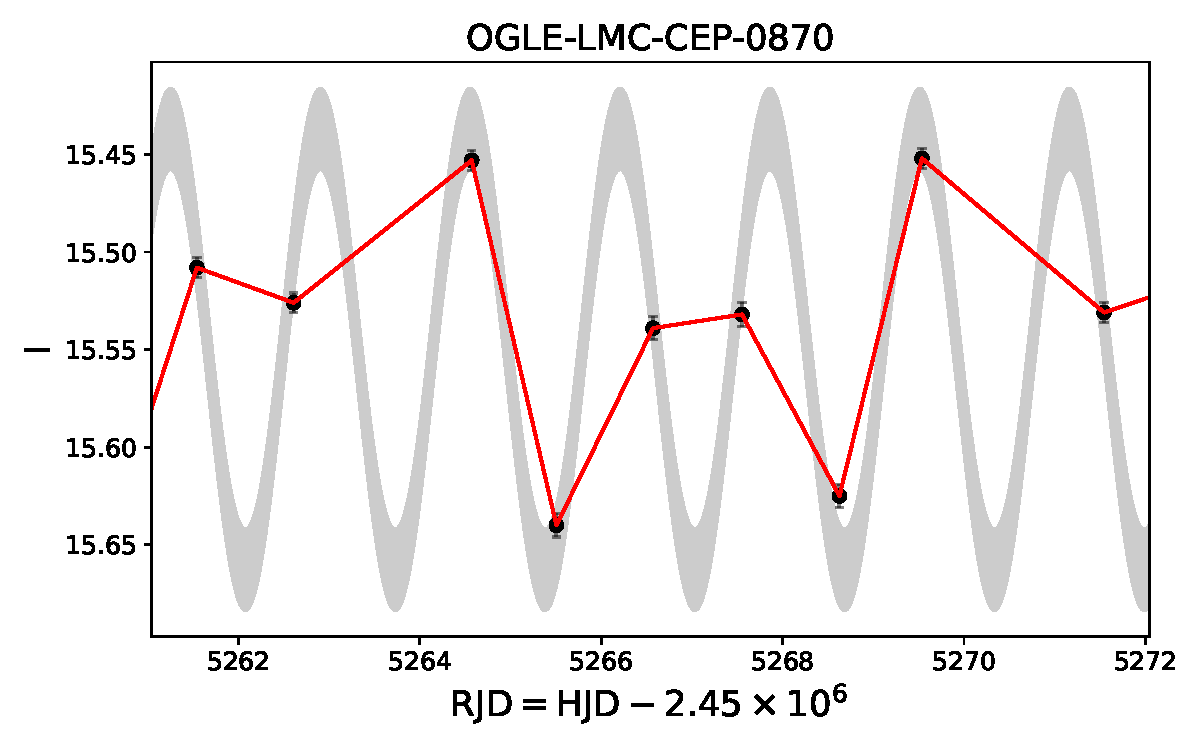
\includegraphics[width=0.7\textwidth]{img/interpolation_failure.pdf}
		\caption[Failure of interpolation of a light curve]{
			First points of the I band time series for a randomly selected star with low period from the OGLE database \citep{OGLE2016}.
			Data points are in black, and the actual light curve (Fourier series fit to all data) is shown as a gray band. 
			Simple interpolation is shown in red, showing that there is not enough data for a point-by-point interpolation to represent the underlying function.
		}
		\label{fig:interpolation-failure}
	\end{figure}

	With time and magnitude scales covered, the last definition needed is that of the phase. 
	Astronomical observations taken from the earth surface, ignoring those of the sun, can obviously only taken at night.
	Atmospheric related distortions are less prominent near zenith, 
	so measurements are ideally taken when the star is in its highest point in the sky,
	but telescope times are heavily scheduled, so the measure will be taken whenever possible.
	Additionally, because of the rotation of the earth around the sun, 
	there will be months of the year when the object will not be visible during night.
	
	These irregularities in the measuring times, apart from having consequences on the signal analysis process of the data,
	can obfuscate the phenomenology of the star's light curve, specially if its variability period is on the order of days.
	Continuous measurements $I_{t=0}$,$I_{t=1}$ (approximately one day apart) are not necessarily in the same period, 
	and thus there is no way to grant that the value at an intermediate time (say $I_{t=1/2}$) is even inside the $[I_0,I_1]$ range;
	any interpolation would eventually fail, as it is seen in \autoref{fig:interpolation-failure}.
	

	But as already stated, the shape of the light curve carries phenomenological details about the star variation.
	In order to recuperate that shape without having to fit the data, and if the period is known,
	one can define the \textit{phase} $\phi$ of a certain time $t$ as
	\begin{equation}
		\phi(t) = \frac{\text{mod}(t-t_0,P)}{P} = \text{mod}_1\left(\frac{t-t_0}{P}\right) \label{eq:phase}
	\end{equation}
	where $t_0$ is called the ephemeris time, and is commonly taken as the point with maximum brightness (minimum magnitude).
	The first definition is just the time that has passed since the last maximum divided by the period, 
	and the second is the fractional part of the time since \textit{any maximum}\footnote{
		By properties of the mod function, the phase remains the same if $t_0$ is shifted by any whole multiple of $P$.
	} in units of $P$.
	
	A phase diagram is then a plot of the phase against the magnitude. 
	Examples can be found on \autoref{fig:mag-phase-1} and \autoref{fig:mag-phase-2}.
	
	The condition that the period has to be known to properly make a phase diagram can seem ridiculous, 
	since the purpose of this work is to find periods.
	But this ends up playing in our favor: 
	it is precisely the fact that phase diagrams are only correct in the period that will allows us to find the period using phase diagrams.
	The discussion about how the phase diagram behaves on a wrong period and how that can be used to find the correct one is presented on \autoref{sec:phase-diagram-methods}.
	
	\begin{figure}
		\centering
		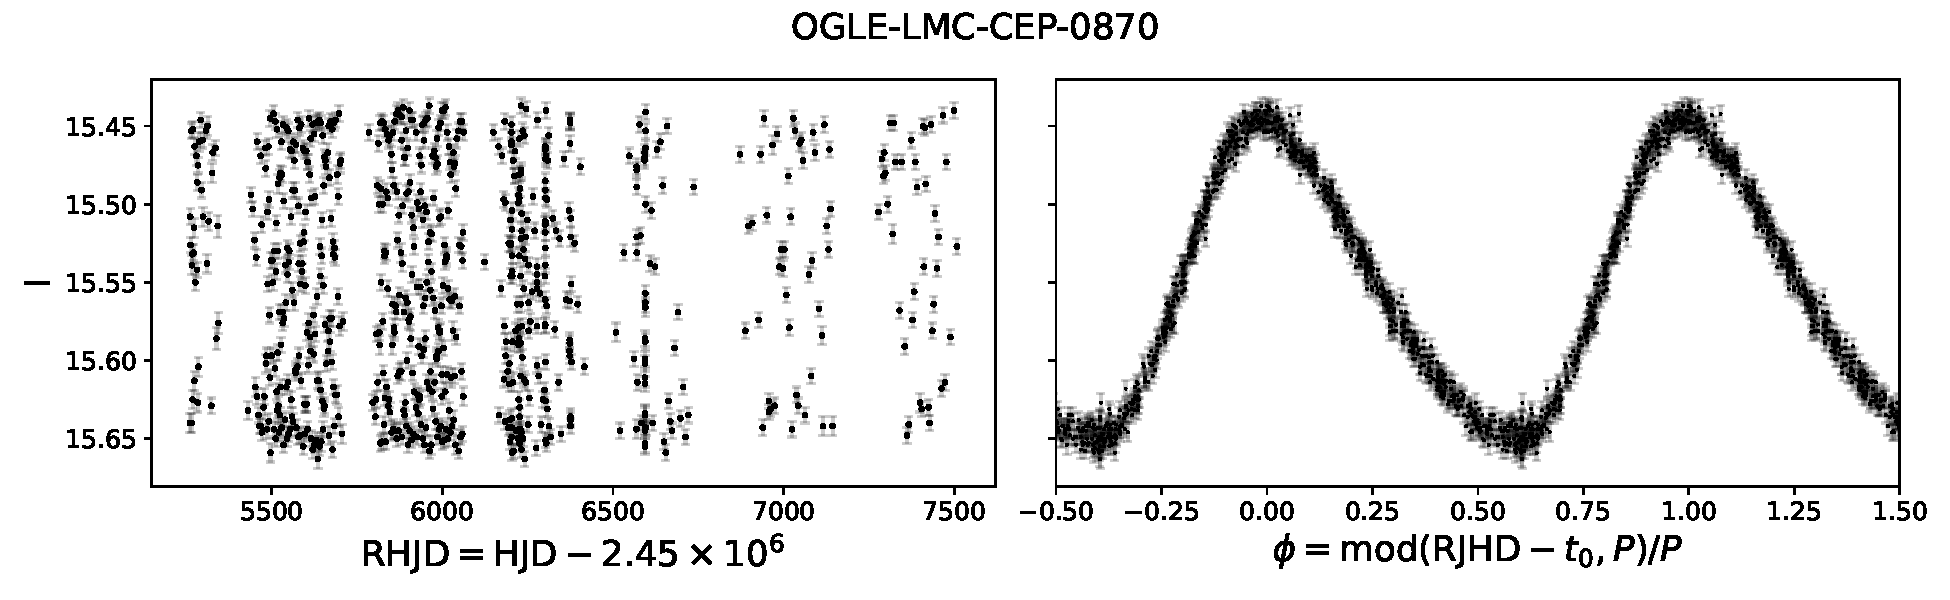
\includegraphics[width=\textwidth]{img/mag_phase_LMC_0870.pdf}
		\caption[Light curve of OGLE-LMC-CEP-0870]{
			I band time series and phase diagram for a randomly selected star with low period from the OGLE database \citep{OGLE2016}.
			Uncertainties for the magnitudes are shown as light gray error bars.
			Temporal units are ephemeris days, and ephemeris time $t_0$ is taken as the time with minimum magnitude.
			A period of $P=1.6518$ days was used for the phase.
			The yearly windows when the object cannot be observed from the ground observatory are clearly present in the time series.
		} 
		\label{fig:mag-phase-1}
	\end{figure}
	
	
	\begin{figure}
		\centering
		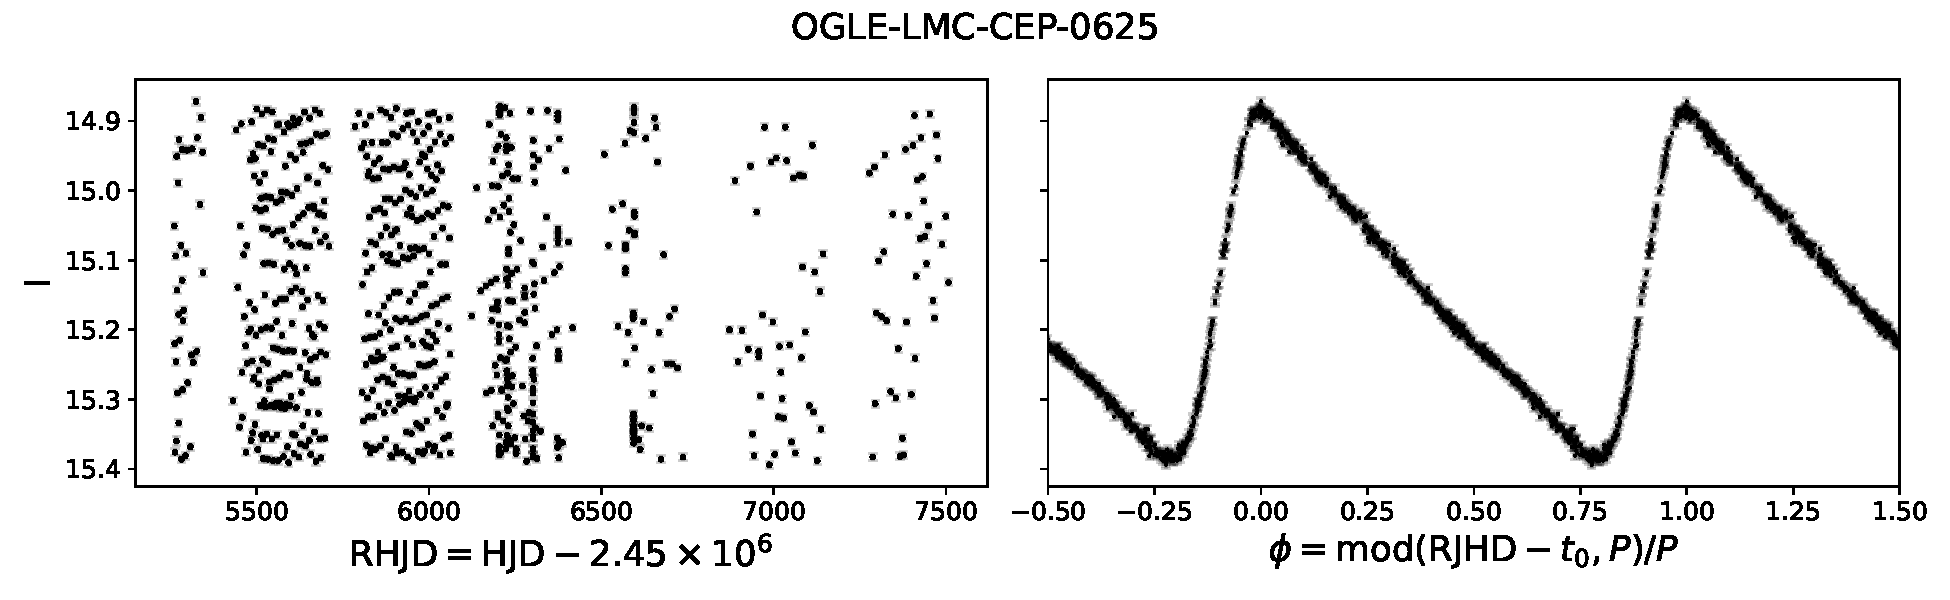
\includegraphics[width=\textwidth]{img/mag_phase_LMC_0625.pdf}
		\caption[Light curve of OGLE-LMC-CEP-0625]{
			Same as in \autoref{fig:mag-phase-1}, but for a typical Cepheid in the LMC. 
			A period of $P=3.7503$ days was used for the phase.
			Phases are padded cyclically for values outside the $[0,1]$ range for clarity, to better observe the behavior of all parts of the light curve.
			Data from \cite{OGLE2016}. 
			A notable difference of this figure and \autoref{fig:mag-phase-1} is the amount of \enquote{dispersion} or width of the light curve.
			This dispersion is much larger than the experimental uncertainty, and should be intrinsic to the star, 
			a phenomenon which deserves further study.
		}
		\label{fig:mag-phase-2}
	\end{figure}
	
	
\section{Cepheid Variable stars}
	
	Classical Cepheid are radial pulsating variable stars, 
	named after the prototypical $\delta$ Cephei as discussed in \autoref{sec:intro-stellar-variability}.
	But that can be a bit misleading, 
	as the term actually refers to an evolutionary stage that some stars present even multiple times in their lifespan.
	Some stars (depending on their mass) leave the main sequence as their Hydrogen fuel gets consumed,
	and evolve into what is known as the instability strip (see \autoref{fig:HR-diagram-karttunen}).
	Cepheids are yellow giants or supergiants at this point \citep{Catelan2015}, and began to experience radial pulsation,
	typically with a period of 1 to 50 days, changing their brightness with amplitudes ranging from 0.1 to 2.5 magnitudes,
	and going from spectral type F to G or even K \citep{Karttunen2017}.
	Their masses can vary from $\sim1 M_\odot$ to $20 M_\odot$, and their radius from $\sim10R_\odot$ to $200R_\odot$
	
	The former are the characteristics of galactic Cepheids, 
	but it is known that there are extra-galactic Cepheids with shorter and larger periods, 
	specially in the Magellanic system \citep{Payne1967,Cox1980}. 
	The data taken by the OGLE project is in agreement with that ranges; see \autoref{sec:data} for more details.
	
	
	\begin{figure}
		\centering
		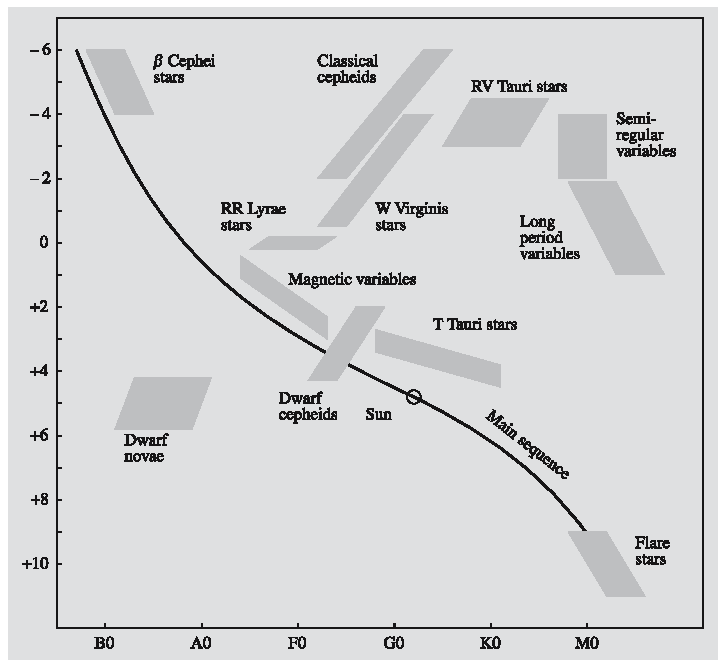
\includegraphics[width=0.7\textwidth]{img/Karttunen_13.2.pdf}
		\caption[Variable stars in the HR diagram]{
			Position of several types of variable stars in a Hertzsprung-Russell diagram.
			The abscissa is given as spectral class, proportional to temperature and color: 
			red (cooler, 3750 K at M0) on the right and blue-white (hotter, 27000 K at B0) to the left. 
			The ordinate is given in absolute visual magnitude $M_V$.
			The main sequence is represented as a solid line, and the Sun as a circle.
			Classical Cepheids can be seen on the red giant branch. 
			Taken from \cite{Karttunen2017}, Figure 14.2.
		}
		\label{fig:HR-diagram-karttunen}
	\end{figure}
	
	\subsection{Stellar populations}
	
	Stars contents are generally classified percentually as Hydrogen ($X$), Helium ($Y$) and \enquote{metals} ($Z$), 
	that constitute really any other element present in the star\footnote{
		For reference, the current surface values for the sun are $X=73.81\%,\,Y=24.85\%,Z=1.34\%$ \citep{Asplund2009}.
	}.
	As the nuclear fusion in the star core turns Hydrogen into Helium, and Helium into heavier elements up to Iron, 
	the balance of the mass fractions over the stars moves from $X$ to $Y$ and eventually to $Z$ as the time passes.
	Moreover, massive stars die in cataclysmic events known as novæ, which have the energy to produce metals heavier than Iron.
	As new stars form from the remnants of the old ones, they have a greater amount of metals from the beginning, 
	but early stars on the Universe would have been mostly Hydrogen, the simplest element.
	
	The idea of the stars coming in generations is attributed to Oort, according to \cite{Baade1944}.
	Baade classified as population I the high metallicity ones (modern value $Z\approx 2\%$), the youngest, 
	and population II the oldest (modern value $Z\approx 0.1\%$) \citep{Carroll2017}. 
	A population III have been theorized since then, those of the first generation of stars, but none have been observed \citep{Heger2002}.
	There is a discussion around the timescales needed for the violent death of the stars to occur (specifically type Ia supernovæ), 
	and if it is sufficient to produce the metallicity difference among populations \citep{Carroll2017}.
	Regardless, the PL relations are dependent on population, and in this work only Cepheids of population I will be considered.
	
	
\subsection{Radial stellar pulsation}
	
	\subsubsection{The period-density relation}

	The most intuitive way of interpreting the radial pulsations of a star 
	is by considering sound-like waves traveling from its center to its surface.
	As a crude approximation, we could consider the equilibrium at the last layer of a star of total mass $M$ and  radius $R$,
	say, a spherical shell of width $dr$ and mass $m\ll M$ at the limit $r\to R$ . 
	Assuming that the pressure outside of the star is zero, and the pressure just below our outer shell is $P$,
	there would be an outward force $P\,A=P\;2\pi r^2$ opposed by the gravitational pull $GMm/r^2$.
	This naive equation of motion would then be
	\begin{equation}
		m \ddot{r} = P 4\pi r^2 - \frac{GMm}{r^2} \label{eq:period-density-motion}
	\end{equation}
	After a painful process of linealization, we will get an equivalent to the Linear Adiabatic Wave Equation (LAWE):
	\begin{equation}
		-\frac{1}{r^4 \rho} \frac{d}{dr}\left(\Gamma_1P r^4 \frac{d\eta}{dr}\right) - \frac{1}{\rho r}\left(\frac{d}{dr}\left[\left(3\Gamma_1-4\right)P\right]\right)\eta = \omega^2 \eta \label{eq:lawe}
	\end{equation}
	where perturbations on $r$ of the form $\xi = \eta e^{i\omega t}$ have been considered, $\rho$ is the mean density and $\Gamma_1$ is the first adiabatic exponent\footnote{
		$\Gamma_1=5/3$ for an ideal gas, and it is the value recommended by \cite{Cox1980}. 
		Interestingly enough, $\Gamma_1=4/3$ for radiation, and the period actually diverges if one blindly uses \autoref{eq:period-density-relation}.
	}. This is equation~5.90 of \cite{Catelan2015}, where the whole linealization process can be consulted.
	\autoref{eq:lawe} is a more general form of that first derived by \cite{Eddington1918}.
	As already stated, the perturbations on the radius are assumed as outward waves with amplitude $\eta$ and angular frequency $\omega$.
	In our simplistic model, the amplitude does not depend on the position of the spherical shell, so $\frac{d\eta}{dr}=0$, and the first term vanishes.
	We shall take away all the radial dependencies, except of course for that of the pressure, as we are considering sound waves:
	\begin{equation}
		\left(\frac{3 \Gamma_1-4}{R\rho}\right)\left(-\frac{dP}{dr}\right) = \omega^2 \label{eq:lawe-result}
	\end{equation}
	That pressure dependence comes from the pressure gradient equation of stellar evolution (in its hydrodinamical from) \cite[equation 4.18]{Catelan2015}:
	\begin{equation}
		\ddot{r} = -\frac{1}{\rho} \frac{d P}{d r}-\frac{GM}{r^3}
	\end{equation}
	which we can use in equilibrium ($\ddot{r}=0$) on \autoref{eq:lawe-result} to get
	$$
	\omega^2 = (3\Gamma_1-4)\frac{GM}{R^3}
	$$
	And in terms of the period $\Pi$ and the mean density $\rho=M/(\frac{4}{3}\pi R^3)$
	\begin{equation}
		\Pi = \frac{2\pi}{\sqrt{(3\Gamma_1-4)\frac{4}{3}\pi G \rho}} \label{eq:period-density-relation}
	\end{equation}
	
	This is usually just a rough estimation of the order of magnitude of the period. 
	For instance, the parameters for $\delta$ Cephei would be $M=4.5\pm0.3 M_\odot$, $R=44.5R_\odot$ \citep{Matthews2012},
	which assuming ideal gas for $\Gamma_1$ gives $\Pi=16.2\pm0.5$ days. 
	The real period is $5.366249$ days \citep{Samus2017}.
	As seen below these oscillations are not necessarily adiabatic, and the amplitude should actually decay.
	

	\subsubsection{The Eddington valve and the $\epsilon$, $\kappa$ and $\gamma$  mechanisms \label{sec:eddington}}
	
	Through the 20th century \cite{Eddington1918,Eddington1926,Eddington1941} 
	proposed a thermodynamic cycle to be responsible for the radial pulsation of stars. 
	He devised two possible physical causes to drive this \enquote{valve}, known today as the $\epsilon$ and $\kappa$ mechanisms.
	
	The $\epsilon$ mechanism is based on the idea that the nuclear processes at the core of the star 
	are more intense in the contraction than in the expansion phase of the valve.
	This would increase the pressure of the stellar material in the contraction phase, 
	and decrease it in the expansion, working in a similar fashion as a Diesel engine \citep{Zhevakin1963}.
	Although it is true that nuclear reaction rates increase with temperature and pressure, 
	this effect only becomes dominant at higher masses ($\sim 100 M_\odot$) and is in fact destabilizing \citep{Carroll2017,Zhevakin1963,Catelan2015}.
	Thus, at least for Cepheids and related variable stars types, the $\epsilon$ mechanisms is not the primary source of radial pulsation.
	
	The second mechanism proposed by Eddington depends on the star stopping 
	the energy leakage from the nucleus when the star is compressed, and allowing that energy to leak when the star expands.
	If the energy is \textit{somehow} retained in the core when the star is contracted,
	the temperature and the pressure will raise, and the star will be forced to expand.
	If then, at the peak of the expansion, the star \textit{somehow} allows that nuclear energy to escape at a higher rate than normal,
	the temperature and pressure in the inside will drop, 
	and the gravitational pull would then win over the pressure gradient, 
	and force the system to began compression again, closing the valve's cycle.
	This would allow the star to pulse without depending on violent variations on the nuclear reaction rates.
	
	But those \enquote{somehow} are quite problematic. Kramers opacity law states that 
	the optical opacity of the stellar material behaves as $\kappa \propto \rho T^{-3.5}$ \citep{Carroll2017}.
	As the dependence is stronger with the temperature, the opacity in the compression phase would be lower, not higher.
	The opacity is directly proportional to the energy (radiation) absorption, and thus the system would not work as Sir Eddington expected.
	
	But there is a way for the temperature changes to be damped at compression and expansion on certain layers of the star. 
	These are called partial ionization zones, and are cause by the increase of degrees of freedom on Hydrogen and Helium gases undergoing ionization \citep{Cox1963},
	which effectively rises the heat capacities $C_V$ and $C_P$ of the layers \citep{Carroll2017}.
	There are two such layers, one where Hydrogen and Helium experience their first ionization:
	$$
		\left.\begin{matrix}
			\text{H I} &\to &\text{H II} & \text{at} & 13.5984345997(02\pm12) \text{ eV} \\
			\text{He I} &\to &\text{He II} & \text{at} &  24.5873890(90\pm25) \text{ eV}
		\end{matrix}\right\} \text{(first ionization)}
	$$
	and one deeper layer where the Helium experiences its second ionization:
	$$
		\text{He II} \to \text{He III}\quad \text{at}\quad 54.4177654(86\pm25) \text{ eV} \qquad \text{(second ionization)}
	$$
	Those energies \citep{NIST_ASD} put all those transitions in the ultraviolet region of the electromagnetic spectrum.
	The ionizations \enquote{leak} a fraction of the energy that otherwise would have been spent on increasing the temperature.
	As the temperature increase is less prominent, the density term in Kramers law dominates, and therefore the opacity increases.
	
	Conversely, in the expansion phase, the ions interact with free electrons, releasing energy that is absorbed by the gas, increasing the temperature.
	As the temperature drop for the expansion is less than expected, the density term dominates again, and the opacity decreases. 
	This two processes are known as the $\kappa$ mechanism, proposed by \cite{Zhevakin1963} and verified by \cite{Cox1963}.
	Moreover, the changes in the heat capacities and the damped temperature gradients causes more heat to flow into those layers,
	positively reinforcing the cycle in which is known as the $\gamma$ mechanism.
	
	The position and behavior of this layers is critically dependent of the temperature, and hence the instability strip discussed before must be almost vertical,
	as \cite{Cox1963} derived theoretically. This can be seen in the position of the Cepheid branch on \autoref{fig:HR-diagram-karttunen}.

	This effect also ---and finally--- explains the asymmetrical variability of the brightness on pulsating stars.
	The amount of luminosity retained by the partial ionization layers depends on their position,
	and it releases when the layers are propelled outwards and its opacity diminishes \citep{Carroll2017}.
	The more energy trapped on the compression phase, the greater the force that would make the star expand,
	and as the opacity has just decreased, the increase of brightness happens faster.
	On the other side, the gravitational pull and the pressure gradient that closes the cycle and causes compression again
	are slower, since all of that energy has escaped in the form of light. 
	
	% ascending and descending branches TODO
	
	% put astrophysical consideration of ascending branch in a caption, new figure TODO
	
	The consensus is that all of those mechanisms do require exceptional conditions to actually work, 
	and that could explain why stellar pulsators are indeed rare in the bulk population of stars in the Universe,
	being approximately one for each $10^5$ stars \citep{Carroll2017}.
	
	\subsubsection{Pulsation modes}
	
	% does a star change its pulsation overtones? TODO
	% polaris
	
	Returning to the intuition of the sound waves of the beginning of the section,
	one could be surprised to know that \autoref{eq:lawe} can actually be solve exactly.
	In fact, it constitutes an special case of what is called a Sturm–Liouville problem.
	As any other physics equation with similar generality, there is an infinite family of solutions,
	and we will not go into the details here; it can be consulted on \S 5.6 of \cite{Catelan2015},
	and more generally on \S  9.3 of \cite{Butkov1968}.
	
	But there are important conclusions derived from the solution of \autoref{eq:lawe}.
	In the first place, it is always the case that $\omega^2$ is a real number, but it can be negative, so $\omega$ is not always real.
	As the waves are defined with $e^{i \omega t}$, imaginary frequencies correspond usually to a cataclysmic behavior of the star.
	We will be concerned with the real frequency case, where the wave act as in oscillatory motion.
	This frequency is called the eigenvalue of the system, say $\omega_n$, and it is associated with an eigenfunction $\eta_n$.
	
	Those eigenfunctions act as basis functions for all the waveforms than could be present in the pulsation of the star,
	in a similar way as the sinusoidal functions act as a basis (the Fourier basis) for the sounds produced in a pipe or a flute.
	Moreover, in the same way a pipe can present harmonics with higher frequencies than its lowest standing wave, 
	each of the $\omega_n$, $n>0$, is a harmonic standing wave pulsating radially onto the star.
	
	Therefore it can (and will) be the case that a star is pulsating primarily in, say, the first harmonic ($\omega_1$), 
	or a combination of the fundamental ($\omega_0$) and other harmonics.
	This is denoted as \texttt{nO}, where \texttt{n} is the harmonic (or Overtone, \texttt{O}) number. The \enquote{zeroth} overtone is denoted \texttt{F}, for Fundamental.
	For instance, a star pulsating in its fundamental and second overtone would be denoted \texttt{F2O}. A first and second and third overtone pulsator would be \texttt{1O2O3O}.
	
	The direct solutions of \autoref{eq:lawe} would be of little to no use for this work, 
	as the observational data only includes the magnitude variation, 
	and it is difficult to translate that into radial motion.
	Nevertheless, in the following section will be described how to analyze the magnitude variability using the Fourier theory, and some additional methods.
	
	
\section{The other spectrum, the pulsation spectrum}

If we wanted to extract information from a periodic signal, 
the most natural thing to do is to check how the signal \enquote{correlates} with certain frequencies.
The pure, ideal, harmonic oscillator would correlate only with a single frequency,
but more complex phenomena could correlate with several frequencies with different intensities,
as if one were to describe several coupled oscillators in terms of their normal modes.

This \enquote{correlation} is not precisely defined at this point, but left as an intuitive concept.
This is done purposefully, as we will present several ways to measure it.
Any function that express the intensity of the correlation of a given signal with a frequency as independent variable
would be called a power spectrum. The terms \textit{spectrogram}, \textit{Fourierogram} and \textit{periodogram} are also used through the literature.

\subsection{Fourier Analysis}

When we say frequency, we mean frequency $\nu$ of uniform rotation in some space, as described by a simple waveform $e^{2i\pi \nu t}$.
The decomposition of a function into a linear combination of regular rotations must be based in the theory of Fourier analysis,
if interrogated well enough. 

Then, we will define the basics of the theory. If we have a theoretical signal $f(t)$, that is mathematically well-behaved,
its representation in frequency space would be given by the function
\begin{equation}
	F(\nu) = \int_{-\infty}^\infty f(t) e^{2\pi i \nu t} dt \label{eq:fourier-transform}
\end{equation}
and its called the Fourier transform. The inverse transformation is given by 
\begin{equation}
	f(t) = \int_{-\infty}^{\infty} F(\nu) e^{-2\pi i \nu t} d\nu
\end{equation}
where we follow the conventions from \cite{Deeming1975}. In general, $F(\nu)$ would be a complex number.
The canonical power spectrum is defined as its magnitude:
\begin{equation}
	P(\nu) = F^\ast(\nu) F(\nu) \label{eq:conjugate}
\end{equation}


	\subsubsection{Discrete non-uniform Fourier transform}
	
	One could be purely practical and force the discretization of \autoref{eq:fourier-transform} to a signal with data $\{t_k,f_k\}$,
	defining $f(t) = \sum_k f_k \delta(t-t_k)$, but I propose to deduce it by a visual construction, building it up from the phase diagram.
	
	In \autoref{eq:phase}, the phase was defined as a dimensionless number; the fraction of the period elapsed since the last maximum.
	As an amount of time relative to the period, it goes from 0 to 1.
	We can translate that to a rotational motion interpretation, by making that temporal phase $\phi$ into an angular one $\psi=2\pi \phi$,
	as if that phase were not seen as the fraction of a period, but as the fraction of a rotation.
	This is made to eliminate the need for a modulus operation. For each data point, our definitions would be
	$$
	\phi_k = \frac{t_k-t_0}{P} = \frac{\omega}{2\pi}(t_k-t_0) \qquad \psi_k = \omega(t_k-t_0)
	$$
	That way, the angular phase $\psi_k$ corresponds to the argument of a typical sinusoidal function $\sin(\omega(t_k-t_0))$.
	The phase diagram was a (temporal) phase against magnitude plot, but we can construct a polar plot with these $\phi_k$ as angles and the magnitudes ($f_k$) as radii.
	Such comparison of linear-to-angular representations can be seen in \autoref{fig:complex-phase}.
	One could call this polar plot a \enquote{Fourier curl}, or also a \enquote{complex phase diagram};
	as it is composed of the points $\{f_k \cos(\omega(t_k-t_0)),f_k \sin(\omega(t_k-t_0))\}$, 
	anyone would be tempted to just define it using Euler's formula in the complex plane as $f_k e^{i \omega (t_k-t_0)}$.
	
	\begin{figure}
		\centering
		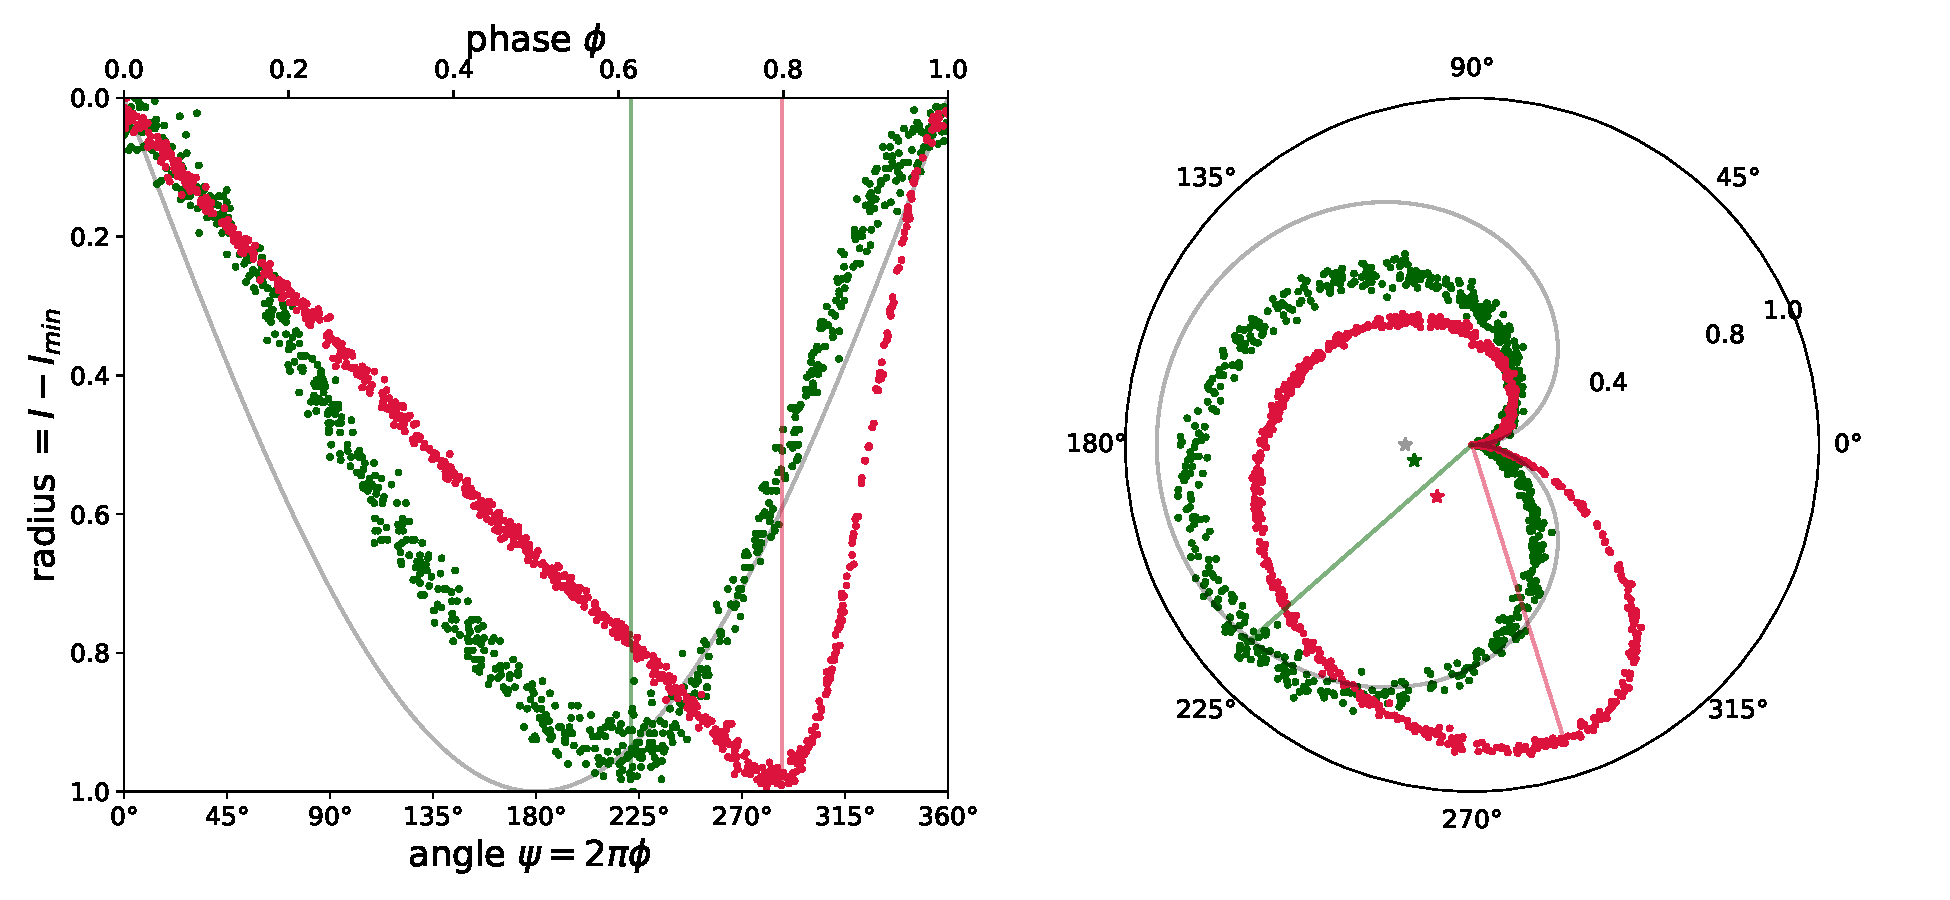
\includegraphics[width=\textwidth]{img/complex_phase.pdf}
		\caption[Complex phase diagram: Fourier curl]{
			Normal and polar phase diagrams for the sample stars in \autoref{fig:mag-phase-1} and \ref{fig:mag-phase-2}, 
			in green and magenta respectively. A simple sine curve is shown in light grey as reference.
			The magnitude was normalized to the $[0,1]$ range for visibility. 
			In the phase diagram, brighter is up. In the polar diagram, brighter is towards the center, and dimmer the larger the radius.
			A transparent line was drawn from the zero of each axis to the point of minimum brightness, for reference.
			In the polar plot, a $\star$ sign represents the centroid of each of the curled data.
			It is of note how the symmetric sinusoid curls up to a cardiod.
		}
		\label{fig:complex-phase}
	\end{figure}
	% augment with off phasing like \ref{fig:offphase} TODO 
	% row of phase
	% row of polar
	
	If the data were to be flat, or just random, one would expect the points in the polar plot to be distributed on an uniform fashion.
	On the opposite case, when the signal is just a sine wave, the polar figure would be a cardioid. 
	The middle case of just a periodic function with relatively low noise is pictured in \autoref{fig:complex-phase}.
	There is a definite clump of points in one direction.
	The most natural way to discern between noise and patterns in this case would be to look at the centroid of the curled figure. 
	In the complex plane this is just the mean of the points:
	\begin{equation}
		C = \frac{1}{N}\sum_{k=1}^N f_k e^{i \omega (t_k-t_0)} \label{eq:centroid}
	\end{equation}
	If we drop the $1/N$ factor and the ephemeris $t_0$, and express it in normal frequency terms $\nu=\omega/(2\pi)$, we get the general discrete Fourier transform:
	\begin{equation}
		F(\nu) = \sum_{k=1}^N f_k e^{2\pi i \nu t_k} \label{eq:fourier}
	\end{equation} 
	as defined by \cite{Deeming1975,Thomson1971,Schuster1898}. 
	The power spectrum in this case would be proportional to the magnitude of the centroid of the Fourier curl, 
	and therefore the independence from $t_0$ is justified.
	
	Provided that there are enough points, and perhaps more importantly, sufficiently wide in time, 
	if $\nu$ were not to be the correct frequency for the signal, the polar plot would be misaligned.
	That is, it would have several \enquote{petals} along all angles, like a rose curve,
	which means that the centroid would be displaced towards the center, its magnitude becoming smaller.
	The more \enquote{correlation} a signal has with a given frequency, the better the alignment of the figure in the polar plot;
	the points with larger radii will clump to one side, and the magnitude of the centroid will be maximum, as can be observed in \autoref{fig:complex-phase-off}.
	
	\begin{figure}
		\centering
		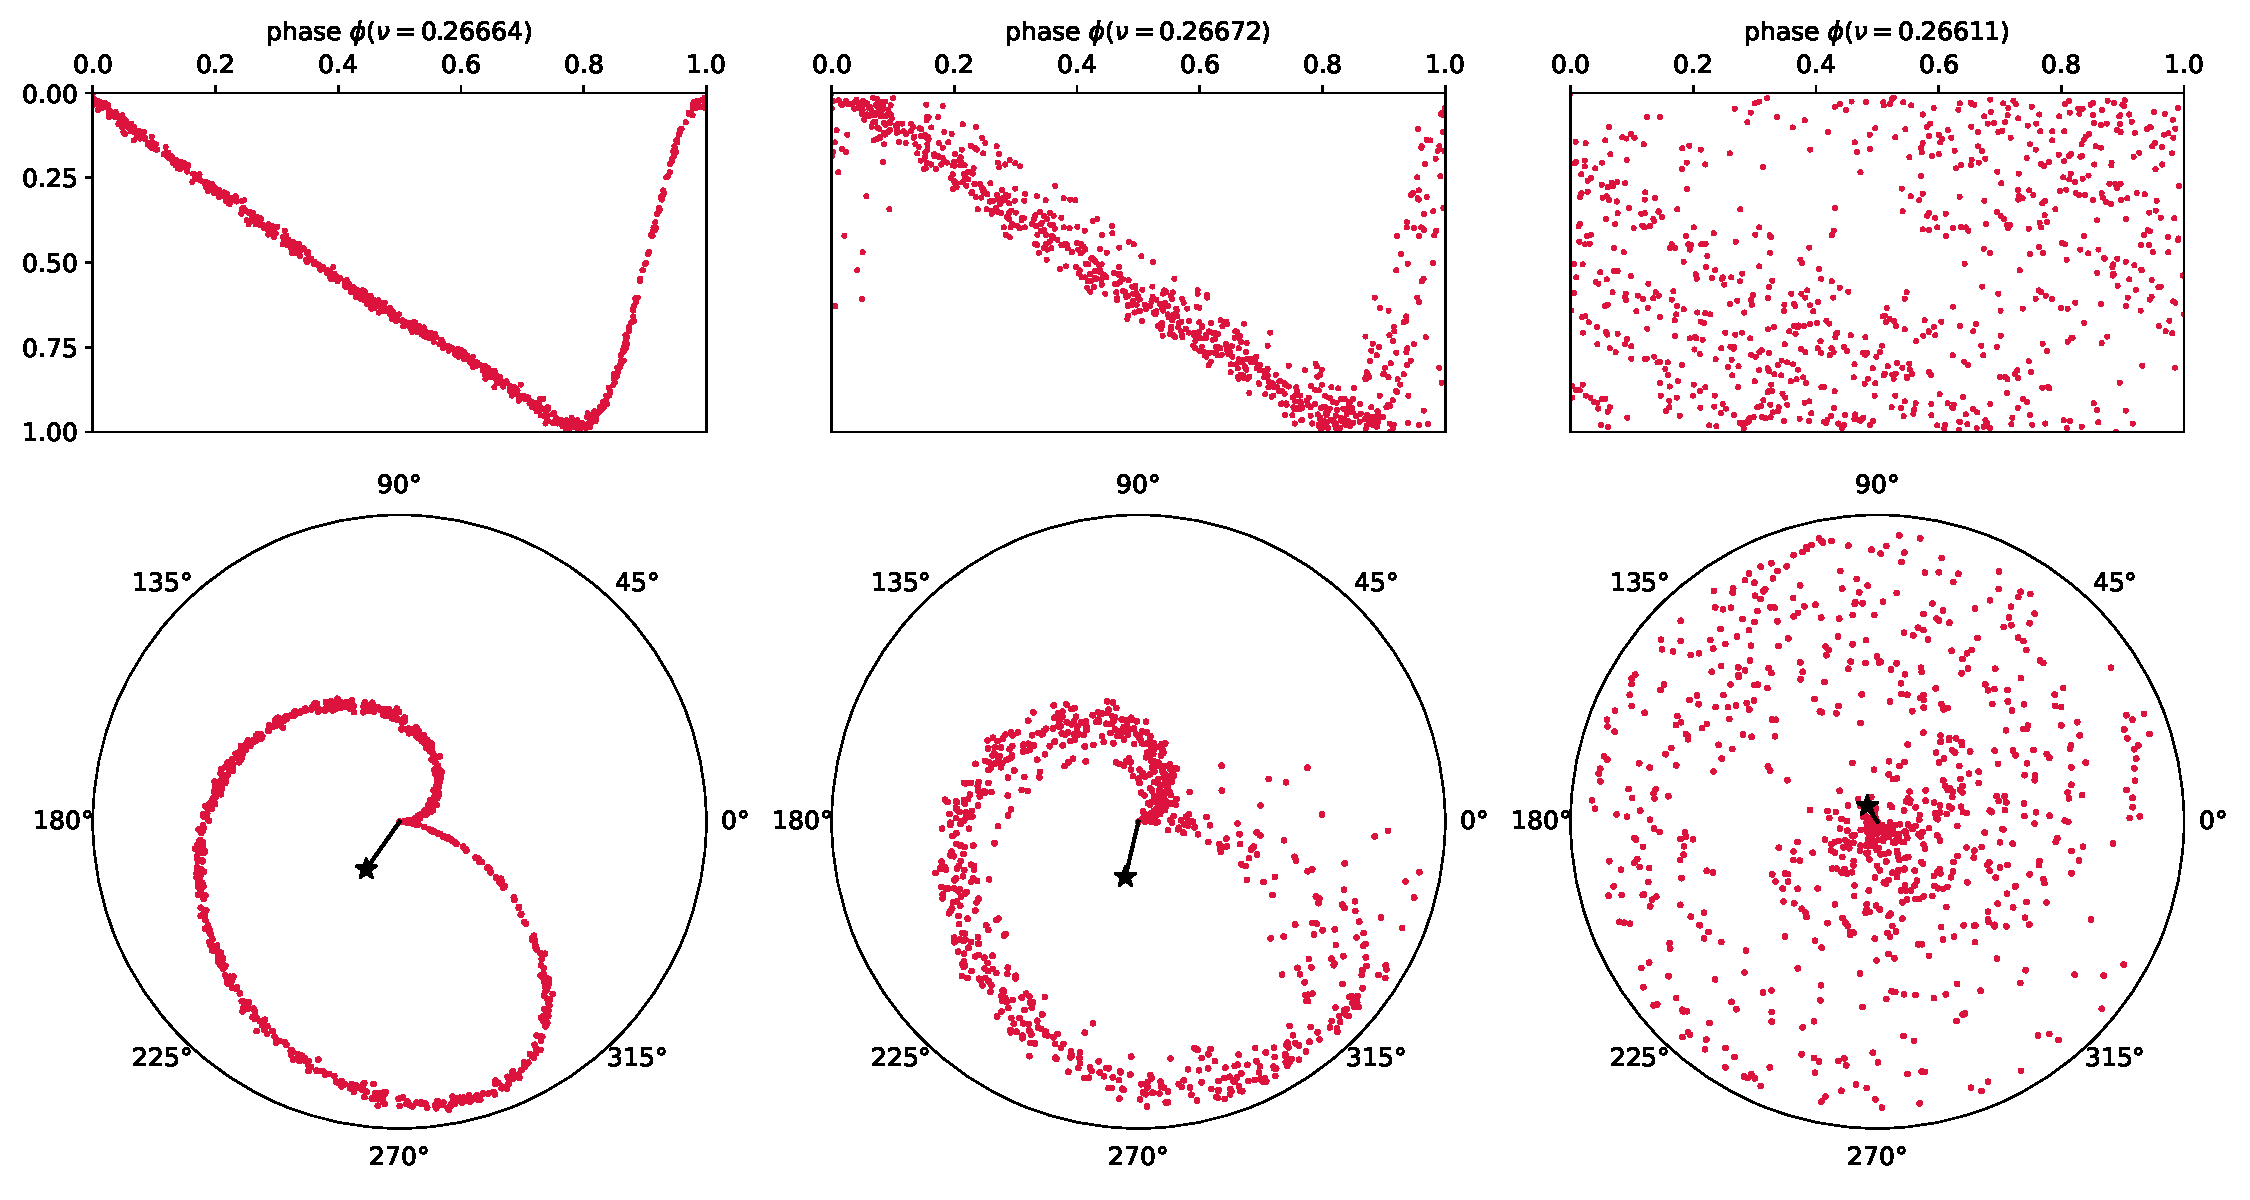
\includegraphics[width=\textwidth]{img/complex_phase_off.pdf}
		\caption[Off-frequency phase diagrams: real and complex]{
			Several phase diagrams (Fourier curls) calculated with different sample frequencies for the star in \autoref{fig:mag-phase-2}.
			Each colum has the normal phase diagram and the polar one. A black line and a star ($\star$) symbol represents the centroid of the curled figure.
			The first column has the correct frequency, and thus the points are clumped together.
			The second column has a frequency only slightly higher; the figure begins to misalign, 
			but the magnitude of the centroid is mostly stable: this periodogram is not as sensitive as the others.
			The las column has a \enquote{completely wrong} phase, despite having two correct decimals.
			The data is distributed more or less uniformly along the angles, and therefore the centroid is almost at zero.
		}
		\label{fig:complex-phase-off}
	\end{figure}
	
	A power spectrum calculated this way would have a peak at the principal frequency, and smaller peaks in the harmonics of the signal.
	In theory, these peaks of the power spectrum are invariant over scale changes, 
	but in practice their widths and heights would depend on the particularities of the data.
	
	As this method involve just a sum over the data, it is expected to be $O(n)$,\footnote{
		All time complexities are given per single frequency iteration. 
		Calculating an spectum with $f$ frequencies, the complecity of a single iteration have to be multiplied by $f$.
	} 
	with an overhead due to the complex exponential (or trigonometric) calculations.
	
	But the most important properties of this way of defining the Fourier power spectrum, in contrast with the fast Fourier transform (FFT),
	is the ability to be evaluated in any frequency $\nu$ with some freedom on the sample times $t_k$\footnote{
		There are some limitations in the reliability of the spectrum depending on the sampling frequencies \citep{Marvasti2001},
		but nonuniform sampling seems to mitigate the problem, as will be discussed in \autoref{sec:sampling}.
	}. 
	The FFT requires the data to be evenly spaced on time, and it calculates the power spectrum on an evenly spaced frequency grid \citep{Brigham1974}.
	As we will see in \autoref{sec:data}, astronomical terrestrial data is far from being evenly sampled, 
	and \autoref{fig:interpolation-failure} already stated that interpolation is not an option either.
	
	
	\subsubsection{The Lomb-Scargle periodogram}
	
	Apart from the very theoretical definition of the correlation between a signal and a frequency that we just presented,
	there is an even simpler one. We could define the correlation of the signal $\{t_k,f_k\}$ with a frequency $\nu$ as 
	how well does the signal is fitted by the model
	$$
	f_k + \epsilon_k = A \cos(2\pi \nu t_k +\phi)
	$$
	where $\epsilon_k$ are independent, normally distributed error terms, and $A$ and $\phi$ are the model parameters.
	In the literature the model is often presented as $A\sin(\omega t_k)+B\cos(\omega t_k)$, 
	which is completely equivalent, as both are forms of a first order Fourier series.
	After the least squares minimization, the coefficient of determination of the fit is given by \citep{Lomb1976,Scargle1982}
	\begin{equation}
		R^2(\omega) \propto \frac{\left(\sum_j f_j \cos\omega (t_j-\tau_\omega)\right)^2}{\sum_j \cos^2\omega(t_j-\tau_\omega)}+
		\frac{\left(\sum_j f_j \sin\omega (t_j-\tau_\omega)\right)^2}{\sum_j \sin^2\omega(t_j-\tau_\omega)} \label{eq:lomb-scargle}
	\end{equation}
	with
	\begin{equation}
		\tau_\omega = \frac{1}{2\omega}\arctan\left(\frac{\sum_j \sin 2 \omega t_j}{\sum_j \cos 2 \omega t_j}\right)  \label{eq:tau}
	\end{equation}
	This $R^2$ can be thought as a first order approximation of the Fourier spectrum, as is lacking the high order terms,
	but it is good enough to discern the peaks of the spectrum.
	%Because of that, this spectrogram is less noisy, something that could be preferred in some cases.
	
	Cepheid light curves, though, are typically not that sinusoidal, as we have established with emphasis.
	But the maximum of the light curve is periodic, so despite a single sinusoid would not be a good fit for the signal,
	the least bad fit would indeed have the correct period.
	
	For a more detailed explanation on how this definition of the power spectrum works, I suggest reading \cite{Vanderplas2018}.
	The original derivation from \cite{Lomb1976} is clean and instructive too, and provides approximations for \autoref{eq:lomb-scargle} and \autoref{eq:tau}.
	
	With this definition it becomes more clear that, provided there is enough data, 
	the model would go progressively out of phase with the signal if the frequency is off.
	The overall quality of the fit $R^2$ would then decrease significantly, 
	and again the power spectrum will present peaks at the principal frequency and its harmonics.

	Although the complexity on this algorithm seems $O(n)$, the redundant trigonometric calculations would present a significant overhead.

\subsection{Phase diagram methods \label{sec:phase-diagram-methods}}

	\subsubsection{Minimum arclength}
	
	Leaving the Fourier side for the moment, there is a curious technique devised by \cite{Burke1970} 
	and analyzed more in depth by \cite{Dworetsky1983} that uses the phase directly.
	
	If the period used to construct the diagram is slightly incorrect, the phases would shift more and more.
	If two points were very near in the good phase diagram, their distance would increase as the period changes.
	Therefore, one way to directly measure the dispersion of the phase diagram is to join all the adjacent points with a line, and calculate its length.
	Mathematically, the arclength $L$ of the diagram would be:
	\begin{equation}
		L = \sum_{k=0}^{N-1} \sqrt{(f_k'-f_{k+1}')^2+(\phi_k'-\phi_{k+1}')^2} \label{eq:arclength}
	\end{equation}
	where \textit{the phases have to be sorted}, hence the primes. This is important: $\phi_k'$ is \textit{not} the phase of $t_k$, but the $k$-th lowest phase, 
	and $f_k'$ its corresponding magnitude, not the magnitude at time $t_k$.
	Contrary to the Fourier method, $L$ will be maximum with the wrong period and minimum with the correct one.
	A graphic depiction of this arclength is given in \autoref{fig:offphase}.
	
	The square root could be obviated, as any maximum of $\sum_k \sqrt{x_k}$ would be a maximum of $\sum_k x_k$.
	The need for sorting the whole phase array each time the test frequency is changed will make this algorithm less efficient
	compared to the trigonometric operations of the Fourier and Lomb-Scargle periodograms;
	usually the sorting process would be $O(n\ln n)$.
	%The square root could be obviated for speed, but it does not matter.
	%The need for sorting the phase array for each test value of the period\footnote{
	%	Remember, all phases have to be computed again if we change the period. 
	%	This is true for all the methods, including the Fourier ones, but no other requires computing the phases \textit{and} sorting them.
	%} makes this method incredibly slow compare to any other one.
	%Regardless, this method could be used to separate false positives from other methods, 
	%and computing it just a dozen times to select peaks will not be that bad in terms of efficiency.
	
	There is an additional peculiarity of this method: the magnitude scale is numerically different than the phase scale, 
	and therefore magnitude differences would contribute differently than phase ones.
	That is solved by normalizing the magnitude to the interval [0,1], as in \autoref{fig:complex-phase}a,
	but typically the highest contributions to $L$ would be vertical, not horizontal, as can be seen in \autoref{fig:offphase}.
	%This and other problems could be solved by only considering the vertical distance.
	
	\begin{figure}
		\centering
		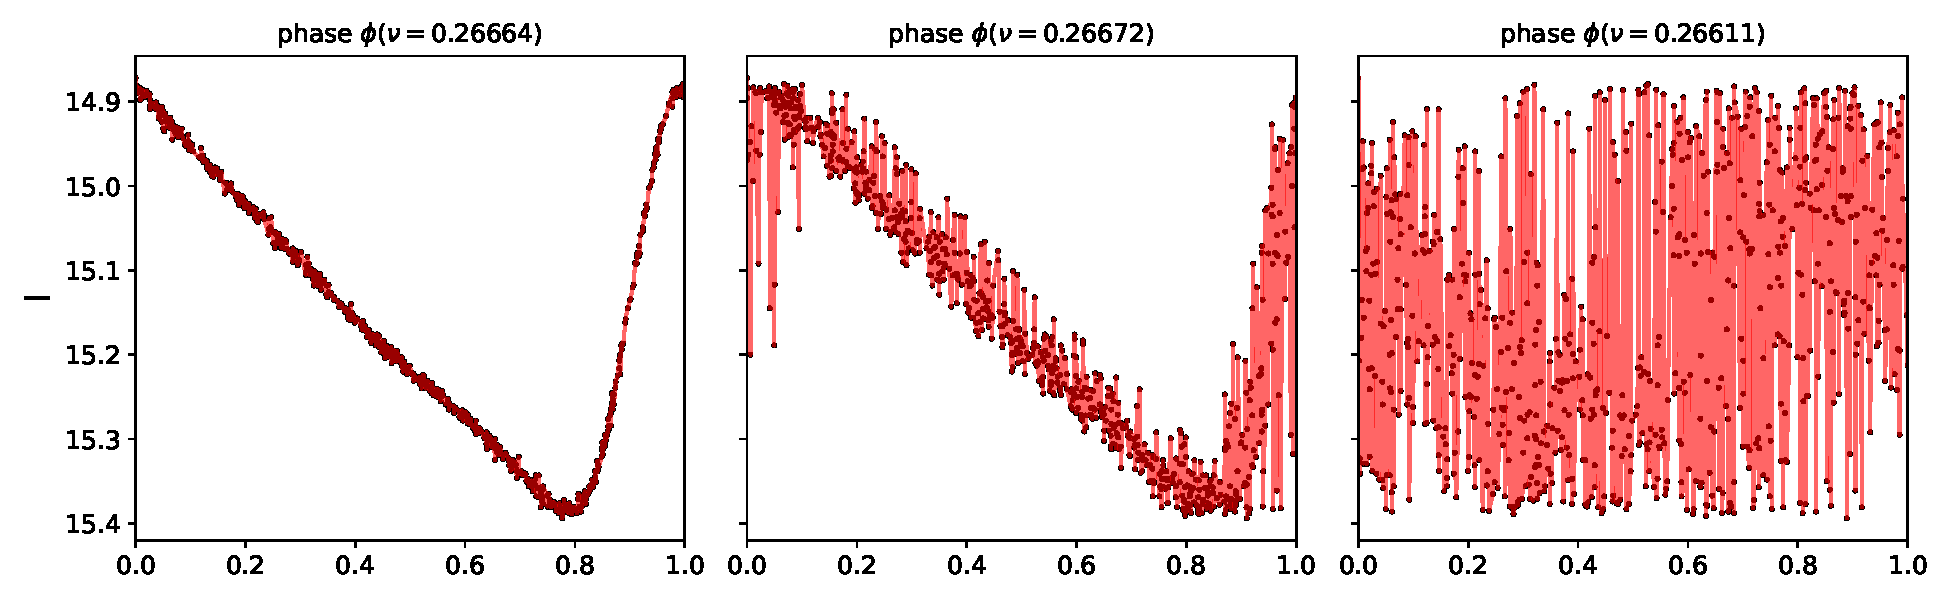
\includegraphics[width=\textwidth]{img/offphase.pdf}
		\caption[Off-frequency phase diagrams: arclength]{
			Different phase diagrams for tests frequencies on the star from figure \ref{fig:mag-phase-2}.
			The red lines are connecting each pair of consecutive dots on the phase diagram,
			and its total length is minimum at the correct phase, and higher otherwise.
			Contrary to \autoref{fig:complex-phase-off}, even the slightest deviation from the correct frequency causes the arclength to rise;
			this method is extremely sensible to phase changes.
		}
		\label{fig:offphase}
	\end{figure}
	
	
	\subsubsection{Phase diagram statistics}
	
	As an alternative to sorting all the phases each time, we could just do it partially,
	dividing the [0,1] phase axis into $M$ equal parts. 
	Then we could use the arclength method with the centroid of the point on those parts, but this does not turn out to be very useful.
	An alternative is the method proposed by \cite{Stellingwerf1978}, which defines the global variance of the phase diagram as
	\begin{equation}
		\sigma^2 = \frac{\sum_k^N (f_k - \bar{f})^2}{N-1}
	\end{equation}
	and a sort of moving variance
	\begin{equation}
		s_j^2 = \frac{\sum_k^{n_j} (f_k-\bar{f}_j)^2}{n_j-1}
	\end{equation}
	where the sum is performed over the $n_j$ points in the $j$-th interval, $j\in[1,M]$.
	The pooled variance for the $M$ samples would be 
	\begin{equation}
		s^2 = \frac{\sum_j^M (n_j-1)s^2}{\sum_j^N n_j -M} \label{eq:pooled-variance}
	\end{equation}
	and the statistic to consider will be defined as $\Theta=s^2/\sigma^2$. 
	If the frequency used to calculate the phases is wrong, $\Theta\approx 1$, and if its right or nearly right, 
	$\Theta$ would reach a local minimum.
	
	This method technically fits the phase curve with the moving mean of the phase curve, and is thus another approximation of the power spectrum.
	The coefficient of determination $R^2=1-\Theta$ could be used directly to compare it with a Lomb-Scargle periodogram, but this method will probably be slower,
	as the tally of a length $n$ array into $M$ sub-intervals is $~O(nM)$.
	
	The same phase diagrams as in \autoref{fig:offphase}, 
	but partially sorted (binned as bidimensional histograms), can be seen in \autoref{fig:offhist2d}.
	Note that this method only requires discretization of the data in the phase axis.
	
	
	\subsubsection{Phase diagram entropy}
	
	If instead of calculating the variance of each column of this histograms,
	we calculate the overall entropy of the data, we would be using the minimum entropy method proposed by \cite{Cincotta1995I}.
	If the phase diagram is partitioned in $m=M^2$ zones of the same area, 
	the probability $\mu_j$ for a point to be inside any given zone is just the points inside that zone divided by the total number of points.
	The entropy of this configuration in the \cite{Shannon1948} sense is 
	\begin{equation}
		S = - \sum_j^m \mu_j \ln(\mu_j) \label{eq:entropy}
	\end{equation}
	As already discussed, if the test period is off, we expect the phase diagram to be populated everywhere; 
	therefore those probabilities would be uniform, and the entropy would be maximum.
	In the correct period the probabilities for each zone are heavily unbalanced towards the occupied spaces,
	and then the histogram is \enquote{ordered} and the information entropy minimum.
	
	On a more mathematical level, if the histogram is populated everywhere, as in the noise case, 
	most of the $\mu_j$ would be nonzero. As probabilities, they lie in the $[0,1]$ interval, 
	making their logarithms negative, adding up to a positive and maximal sum.
	
	On the other side, on the correct period there would be many unoccupied zones (see \autoref{fig:offhist2d}), 
	and therefore most of the $\mu_j$ would be zero. As $\lim_{\mu\to0}\mu \ln \mu = 0$.
	The growth of the other probabilities cannot compensate for this loss, so the sum is minimum.	
	This has been rigorously proved by \cite{Cincotta1999II}.

	As the obvious implementation involve the full bidimensional binning of the phase diagram, 
	this would be $O(nM^2)$, making it technically slower than the other methods.
	There are faster methods to compute the entropy of a signal \citep{Cohen1985}, 
	but for our purposes it is possible to implement an entropy method that is faster that both 
	the $O(n\ln n)$ arclength and the $O(nM)$ method, by transforming the bidimensional histogram into a one dimensional one;
	see \autoref{lst:entropy-flattened} for details.
	
	\begin{figure}
		\centering
		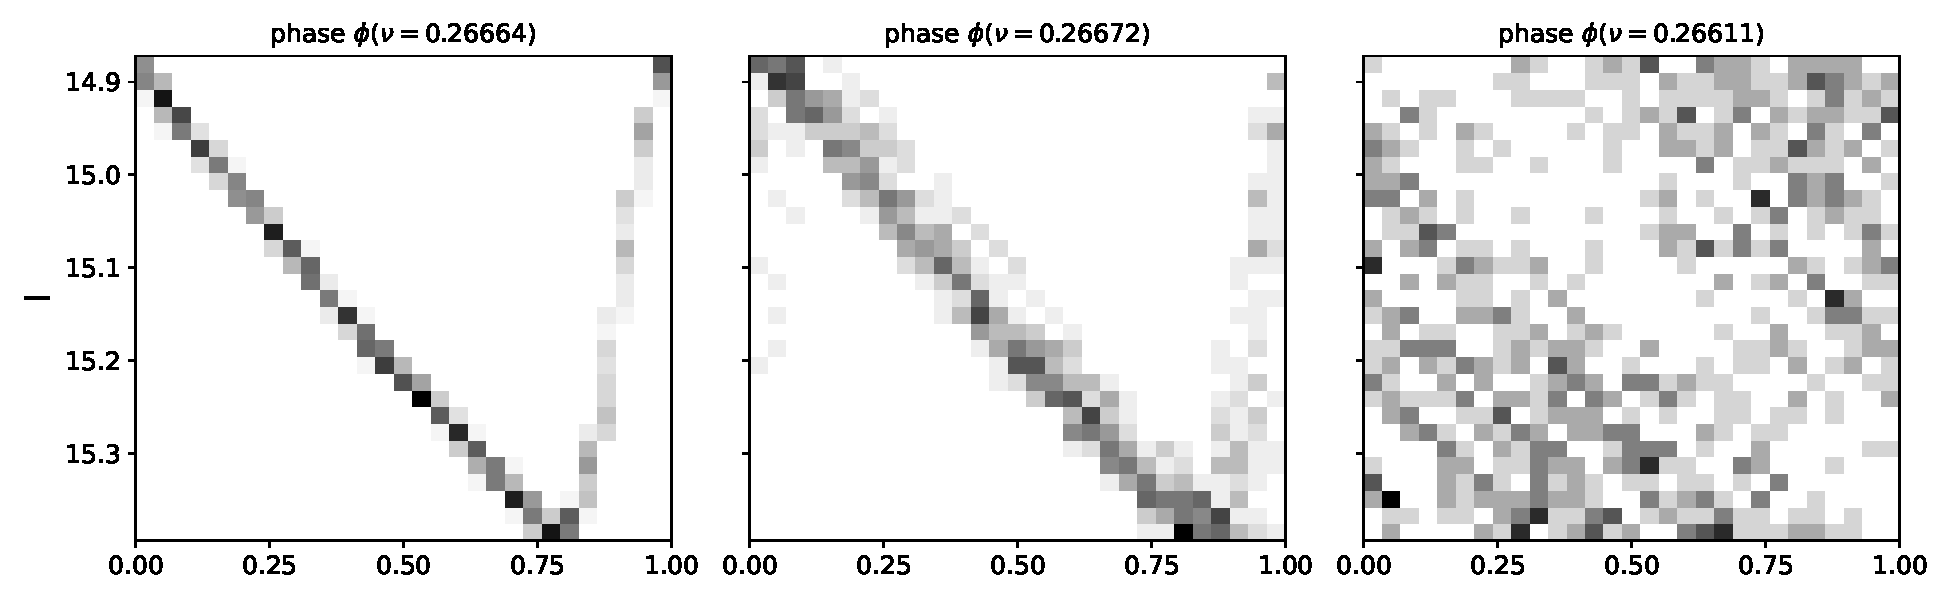
\includegraphics[width=\textwidth]{img/offhist2d.pdf}
		\caption[Off-frequency phase diagrams: histograms]{
			Same as \autoref{fig:offphase} but \enquote{pixelated} phase diagrams, \textit{i.e.} bidimensional histograms.
			$M=30$ bins were taken on each axis, for a total of $m=900$ zones.
			The greater column-wise dispersion of the off-phase diagrams is notable, 
			and when the frequency is completely wrong, the image is just noise.
			On the applications discussed here, the number of bins on each axis are typically between 2 and 10.
		}
		\label{fig:offhist2d}
	\end{figure}




	
	
	
	
	
	
	
	
	
	
	
	
	
	
	
	
	
	
	
	
	
	
	
	
	
	
	
	
	
	
	
	
	
	

\chapter{Methodology}
\section{OGLE IV classical Cepheids on the Magellanic clouds}

\subsection{The OGLE project}

The Optical Gravitational Lensing Experiment (OGLE) project is an earth-based observational astronomical project 
with the objective of study dark matter and microlensing phenomena in the Magellanic clouds and the Galactic bulge.
This project was originated by an idea of Bohdan \cite{Paczynski1986}. 
Its first phase began in 1992, with very limited time in the 1m Swope telescope, in Las Campanas Observatory, Chile,
operated by the Carnegie Institution of Washington.

Those initial observation continued until 1995, and produced many interesting results: 
apart from its initial goal of observing microlensing events \citep{Udalski1993},
they published extinction maps of the galactic bulge \citep{Stanek1996},
and the first version of their catalog of variable stars \citep{Udalski1997}.

The whole idea of Paczyński was a great success despite its difficulties,
and therefore the Warsaw University decided to further fund OGLE.
In 1995 began the construction of the 1.3m Warsaw telescope and observing site at the same observatory, due to its optimal position.
The construction, assembly and tests were concluded by late 1996, 
and in 1997 began the second phase of the project.

Third and fourth OGLE phases began in 2001 and 2010 respectively. 
The last phase, OGLE-IV, is still on pause at the time of writing this document (late 2021) due to the COVID-19 pandemic.
As of 2019, their main site\footnote{\url{http://ogle.astrouw.edu.pl/}} reported $\sim$800 papers published from the main OGLE results,
and $\sim$1300 OGLE-related results. 
All of that makes the OGLE project one of the oldest observational projects that have been focused on the same objects,
making it an invaluable resource for studying the Magellanic system and the galactic bulge.

\begin{table}
	\centering
	\begin{tabular}{l|rrrrrrr}
		mode &     stars &  with I & only I & with V & only V & both &  none \\ \hline\hline
		F      &  2477 &  2428 &       151 &  2287 &        10 &  2277 &    39 \\
		1O     &  1776 &  1766 &       116 &  1650 &         0 &  1650 &    10 \\
		2O     &    26 &    26 &         0 &    26 &         0 &    26 &     0 \\
		F1O    &    95 &    95 &         6 &    89 &         0 &    89 &     0 \\
		1O2O   &   322 &   321 &        16 &   305 &         0 &   305 &     1 \\
		F1O2O  &     1 &     1 &         0 &     1 &         0 &     1 &     0 \\
		1O2O3O &     7 &     7 &         0 &     7 &         0 &     7 &     0 \\
		1O3O   &     1 &     1 &         0 &     1 &         0 &     1 &     0 \\
		2O3O   &     1 &     1 &         0 &     1 &         0 &     1 &     0 \\\hline
		total  &  4706 &  4646 &       289 &  4367 &        10 &  4357 &    50 \\
		%F      &  2477 &  2428 &  2287 &  2277 &    39 \\
		%1O     &  1776 &  1766 &  1650 &  1650 &    10 \\
		%2O     &    26 &    26 &    26 &    26 &     0 \\
		%F1O    &    95 &    95 &    89 &    89 &     0 \\
		%1O2O   &   322 &   321 &   305 &   305 &     1 \\
		%F1O2O  &     1 &     1 &     1 &     1 &     0 \\
		%1O2O3O &     7 &     7 &     7 &     7 &     0 \\
		%1O3O   &     1 &     1 &     1 &     1 &     0 \\
		%2O3O   &     1 &     1 &     1 &     1 &     0 \\\hline
		%total  &  4706 &  4646 &  4367 &  4357 &    50 \\
		\end{tabular}
		\caption[Pulsation mode and filter data distribution for the LMC]{
			Distribution of the number of stars in the database for the LMC according with their reported pulsation mode.
			The first column give the total of stars in that mode.
			The next four columns give how many of those stars have data in $I$ band, \textit{only} $I$ band, and the same for $V$ band.
			The last two columns enumerates the stars that have data in both bands and the stars of which no data were found in the database.
			As can be seen, there are so few stars with pulsation modes F1O2O, 1O2O3O, 1O3O, and 2O3O, 
			that their inclusion in the following analysis would be less than satisfactory.
		}
		\label{tab:LMC}
\end{table}

\begin{table}
	\centering
	\begin{tabular}{l|rrrrrrr}
		mode &     stars &  with I & only I & with V & only V & both &  none \\ \hline\hline
		F      &  2754 &  2739 &       125 &  2617 &         3 &  2614 &    12 \\
		1O     &  1791 &  1783 &        86 &  1697 &         0 &  1697 &     8 \\
		2O     &    91 &    91 &         2 &    89 &         0 &    89 &     0 \\
		F1O    &    68 &    68 &         2 &    66 &         0 &    66 &     0 \\
		1O2O   &   239 &   239 &         9 &   230 &         0 &   230 &     0 \\
		1O2O3O &     1 &     1 &         0 &     1 &         0 &     1 &     0 \\\hline
		total  &  4944 &  4921 &       224 &  4700 &         3 &  4697 &    20 \\
		%F      &  2754 &  2739 &  2617 &  2614 &    12 \\
		%1O     &  1791 &  1783 &  1697 &  1697 &     8 \\
		%2O     &    91 &    91 &    89 &    89 &     0 \\
		%F1O    &    68 &    68 &    66 &    66 &     0 \\
		%1O2O   &   239 &   239 &   230 &   230 &     0 \\
		%1O2O3O &     1 &     1 &     1 &     1 &     0 \\ \hline
		%total  &  4944 &  4921 &  4700 &  4697 &    20 \\
	\end{tabular}
	\caption[Pulsation mode and filter data distribution for the LMC]{
		Same as \autoref{tab:LMC} but for the SMC. 
		This time, there is a single star with pulsation mode 1O2O3O,
		and therefore it will be excluded from the analysis.
		This choice leaves the LMC and the SMC with the same pulsation categories.
	}
	\label{tab:SMC}
\end{table}

\subsection{Data acquisition and description \label{sec:data}}

% instrumentation

As previously mentioned, the OGLE project uses its own 1.3m telescope at Las Campanas Observatory, Chile,
fully described by \cite{OGLEIIinstrumentation}. 
The OGLE-IV phase uses this telescope, and since 2009 they use a mosaic camera of 32 thin E2V44-82 2048×4096 CCD chips,
with 0.26 arcsec/pixel scale and 1.4 square degrees total field of view.
The whole data obtention process, the specific mosaic arrangement and the sky coverage are described by \cite{OGLE2015}.

% description

This work uses a subset of the The Ogle Catalog of Variable Stars (OCVS), publicly available to download for the 
astronomic community at \url{http://www.astrouw.edu.pl/ogle/ogle4/OCVS/}.
Specifically, we will use the photometric data from Classical Cepheids in the Small and Large Magellanic clouds (SMC,LMC).
This section of the catalog is composed of 9583 individual stars, with data on the $I$ and $V$ magnitude, 
taken with the filters shown in \autoref{fig:filters}, but converted to the standard Johnson-Cousins photometric system \citep{OGLE2015}.
Each data file is composed of three columns, the date of the observation in $RHJD=HJD-2.45\times 10^6$, 
the measured magnitude, and its uncertainty. 
Uncertainties though the data varies from $0.004$ mag to $0.1$ mag in the most extreme cases. 
Those cases are extremely rare, however, and the mean stays at around $0.006$ mag.

% missing data and tables

There are some stars that, perhaps by observation schedule, perhaps by reclassification, have no data files in some filters, or have data in only one.
This information, separated by reported pulsation mode, is detailed in \autoref{tab:LMC} for the LMC and in \autoref{tab:SMC} for the SMC.
The stars with no data will be ignored, as well as the rarest pulsation modes.
From those tables is clear that stars with $I$ magnitude data are slightly more prevalent.
In fact, even for a star that has data in both filters, there is usually a lot more $I$ magnitude observation than $V$ ones.
The distribution of data points per star per filter can be seen in \autoref{fig:n-hist}.
Probably the $V$ data was only taken to measure its mean, in order to construct the Wesenheit index,
while the $I$ data was taken both for the mean $I$ magnitude and to calculate the period.

\begin{figure}
	\centering
	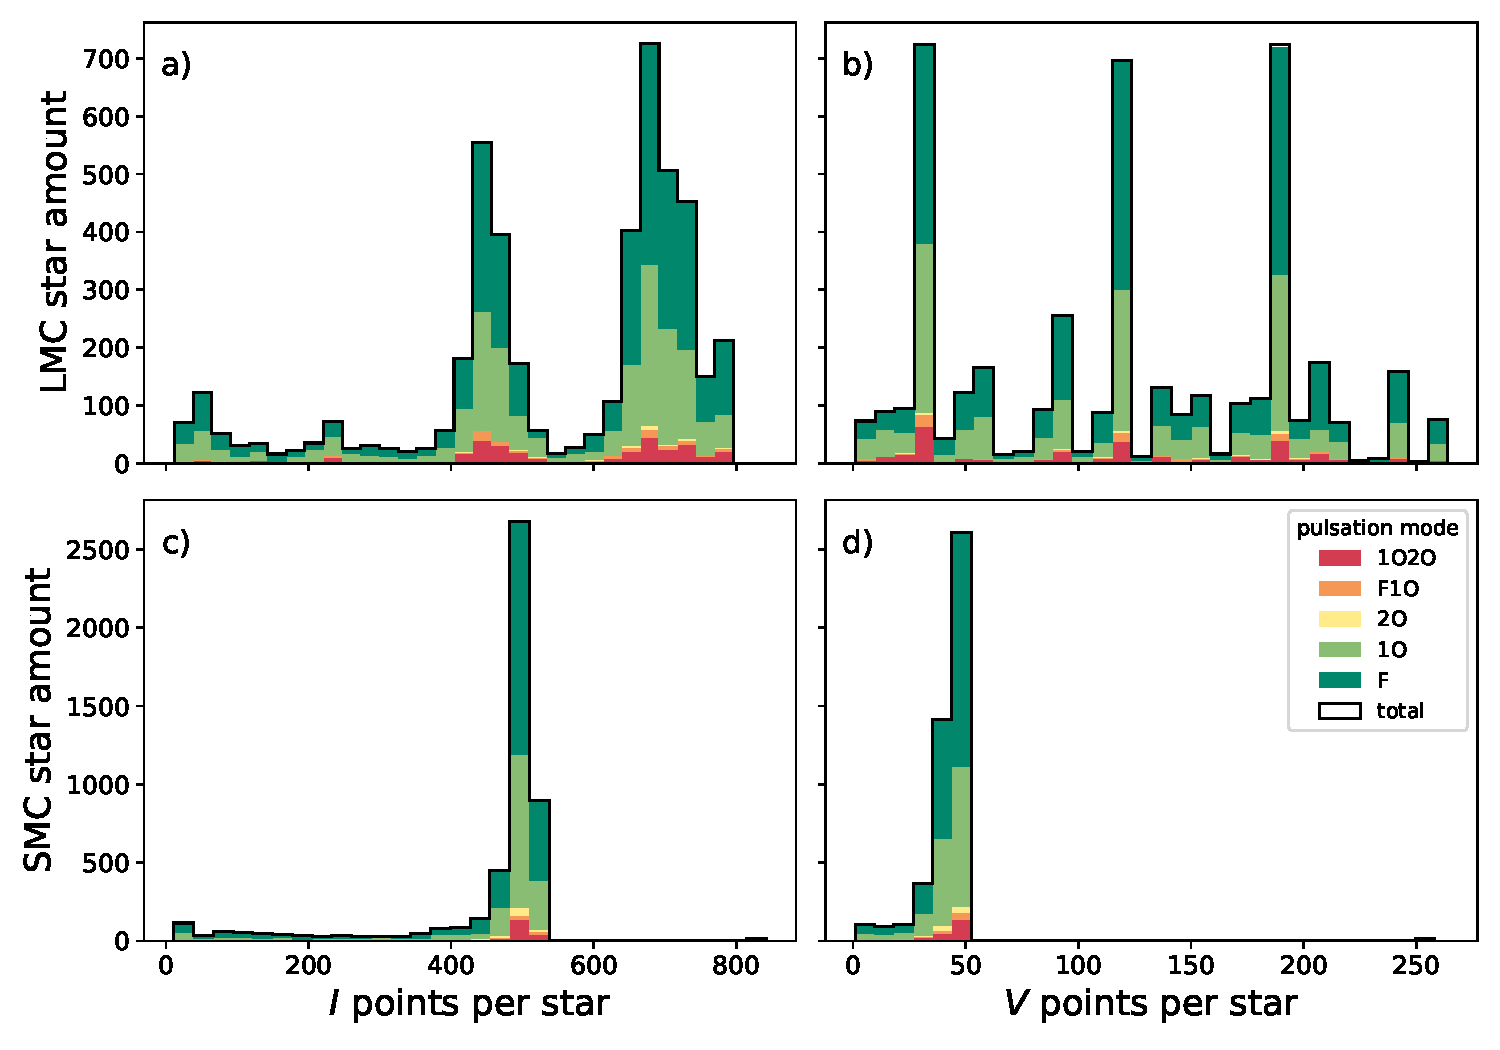
\includegraphics[width=0.9\textwidth]{img/clouds_histogram_ns.pdf}
	\caption[Distribution of data size for classical Cepheids in the Magellanic clouds]{
		Distribution of data points per star in both $I$ and $V$ filters for the LMC and the SMC. 
		Histograms are cumulative, and each color represents the contribution fraction of each pulsation mode on each bin.
		Total is outlined in black.
		As expected, there are much more data points in the LMC compared to the SMC due to their size difference.
		There is also much more data in $I$ magnitude, as outlined in the text.
		The threshold for minimum number of points required by the period finding algorithms is around 50,
		which made the $V$ data unusable for finding periods on the SMC case (d).
		If only $I$ data is to be used for this purpose, 
		the lower tails on both clouds can be cut at around ~400 points without loosing too many stars.
	}
	\label{fig:n-hist}
\end{figure}


% data distributions

In order to define our frequency grid for the period search, the OGLE reported periods can be examined to deduce a reasonable range.
The distributions of $I$ mean magnitude and amplitude can also be examined, as they are all presented in \autoref{fig:pidi-hist}.
There one can see some bimodal behaviors with small tails in the long-period high-luminosity end of the data, 
and sometimes a distinction between the pulsation modes can be made.

\begin{figure}
	\centering
	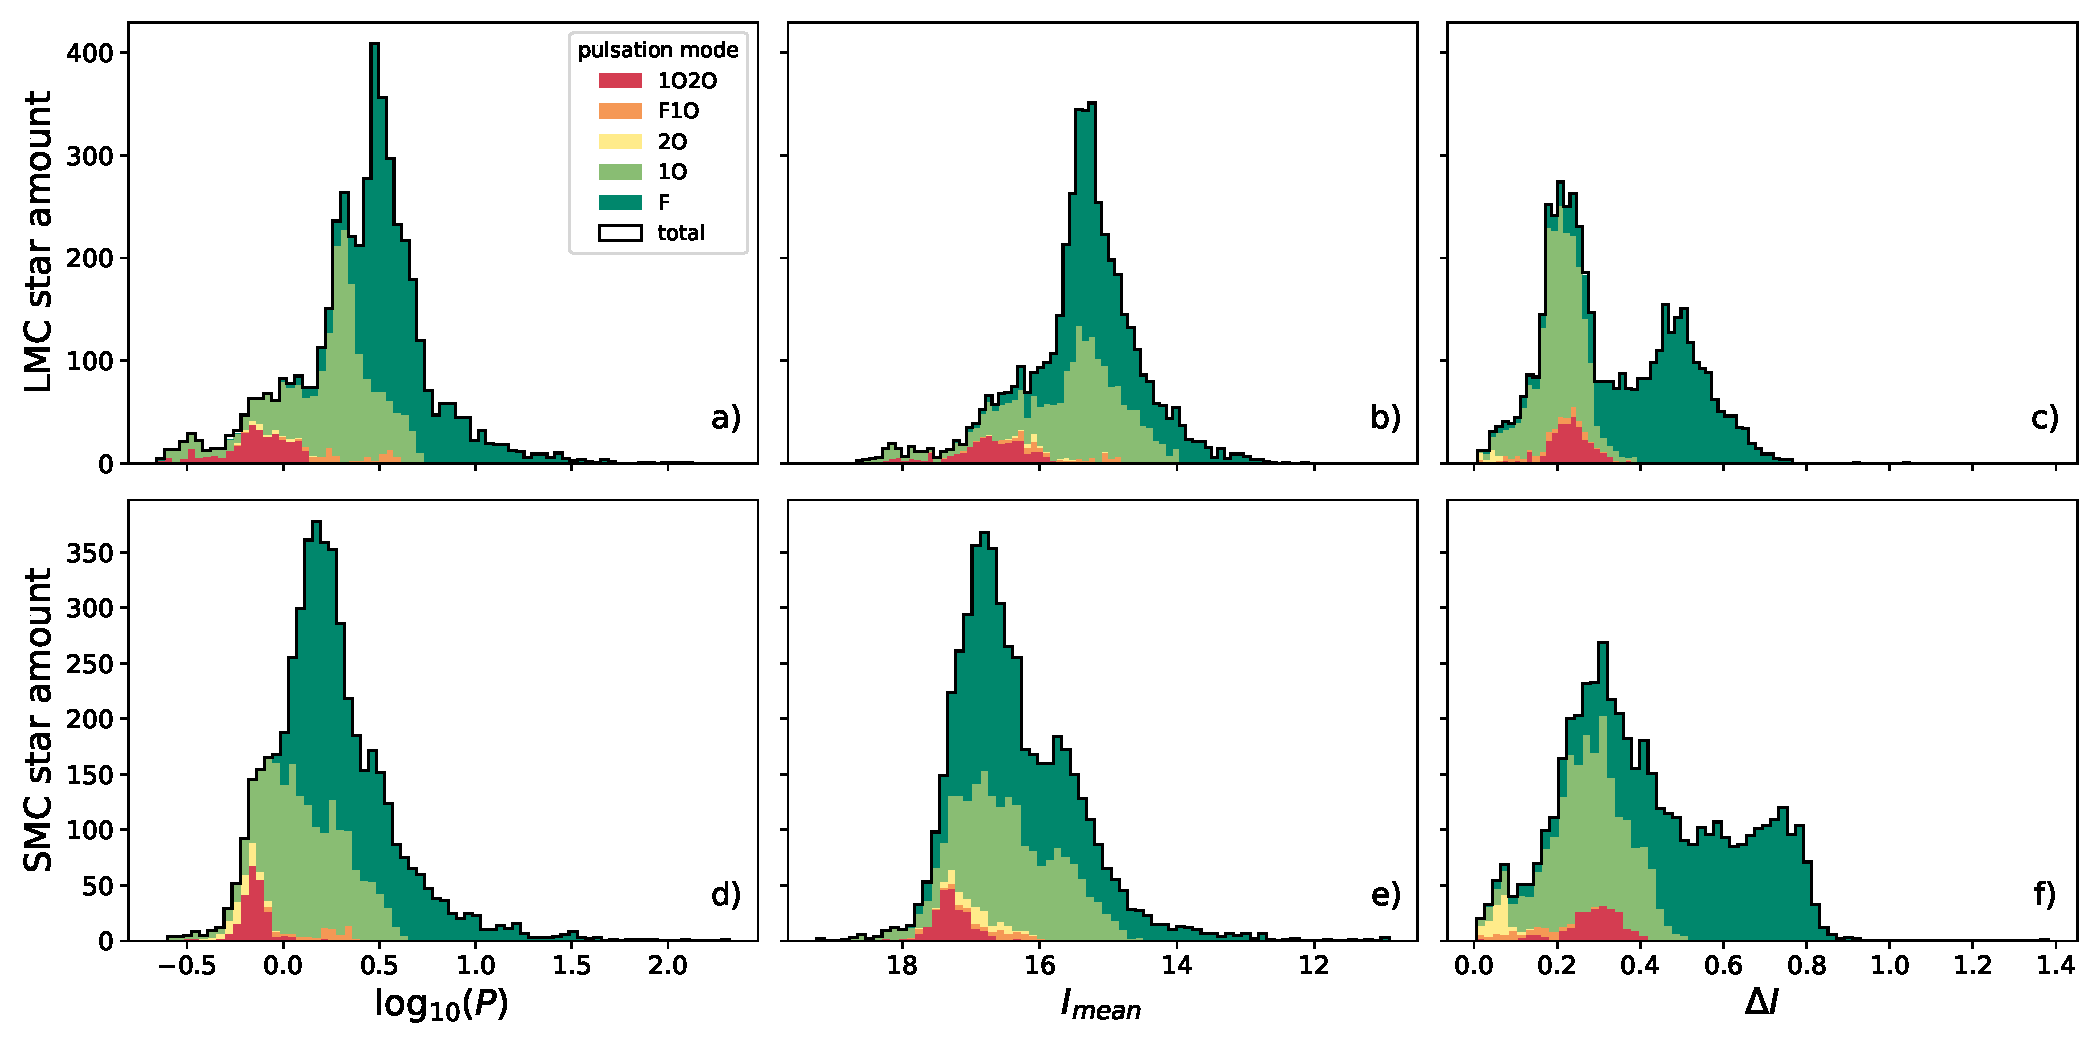
\includegraphics[width=\textwidth]{img/clouds_histogram_PIdI.pdf}
	\caption[Distribution of signal properties for classical Cepheids in the Magellanic clouds]{
		Distribution of periods, mean $I$ magnitudes and $I$ amplitudes for the OGLE classical Cepheids in the Magellanic system.
		Histograms are cumulative, and each color represents the contribution fraction of each pulsation mode on each bin.
		Total is outlined in black.
		In the case of multi-period stars, only the lower one is considered, as reported in the data headers \texttt{*.cep}.
		The tails on the longer periods and brightest and widest stars are kept in the plot range, despite having so few stars,
		to represent the difficulty of studying the bright side of the PL relation.
	}
	\label{fig:pidi-hist}
\end{figure}

% temporal cadence

\subsubsection{Sampling and observation cadence \label{sec:sampling}}

All of these observations are made on earth, and as such,
they are limited to the sky conditions, tight scheduling and the earth rotation.
Therefore, the cadence of observations is far from being evenly sampled.
An example of this uneven nature of the data is presented on \autoref{fig:1234-cadence} for a single star,
and on \autoref{fig:global-cadence} for the whole of OGLE-IV measurements.

As we are not interested in signal reconstruction, but only in finding the true period,
we can bypass the mean sampling frequency limit given by \cite{Marvasti2001}.
In theory, when a signal is evenly sampled, one could only calculate its periodogram up to half that frequency (the Nyquist frequency);
all the subsequent peaks are false peaks, reflections of the spectrum. 
An example of this can be seen on \autoref{fig:uneven-advantage}.

The is shown how uneven sampling might be even beneficial, as one can freely search for a frequency much higher that 
the mean Nyquist limit for the data. How much this effect lasts and hwy many points does it need to be useful remains to bee seen.

\begin{figure}
	\centering
	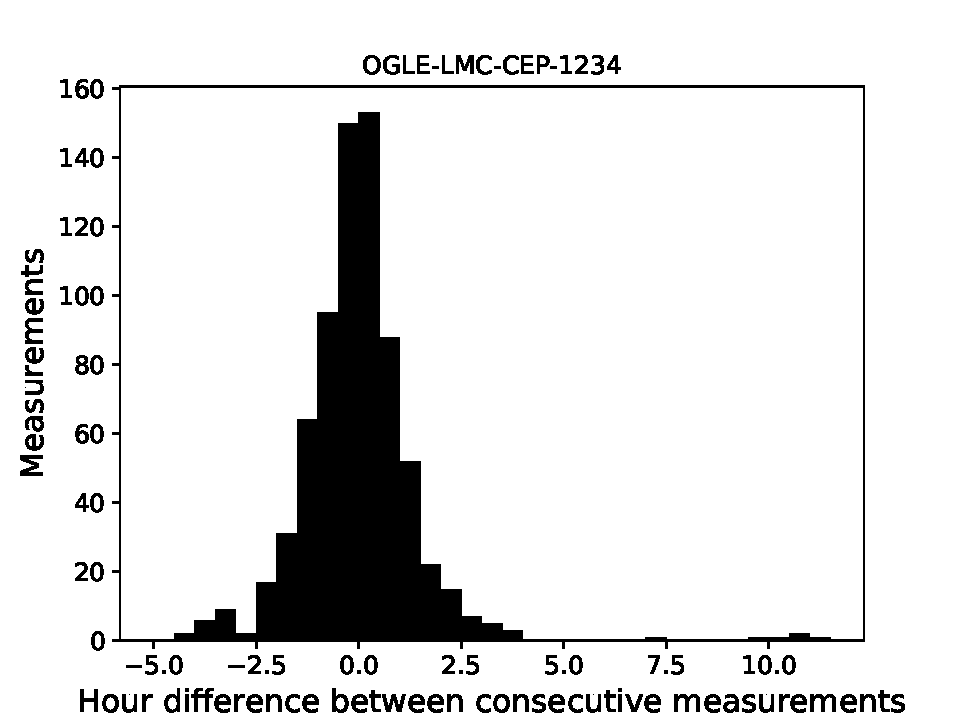
\includegraphics[width=0.5\textwidth]{img/1234_cadence.pdf}
	\caption[Hourly difference between observations for OGLE-LMC-CEP-1234]{
		Histogram of the \textit{hour} difference between consecutive observations for a sample star in the LMC.
		This hour difference is defined as the time difference modulo one day; 
		for example, if one observation was made on Monday at 1:00am, and the next on Tuesday at 3:00am, the hour difference would be 3.
		The small clump on $\sim$10 hours is due to the yearly pauses on observations, as can be seen on Figures \ref{fig:mag-phase-1} and \ref{fig:mag-phase-2}.
		If the data were to be evenly sampled, this histogram would look like a delta function.
	}
	\label{fig:1234-cadence}
\end{figure}


\begin{figure}
	\centering
	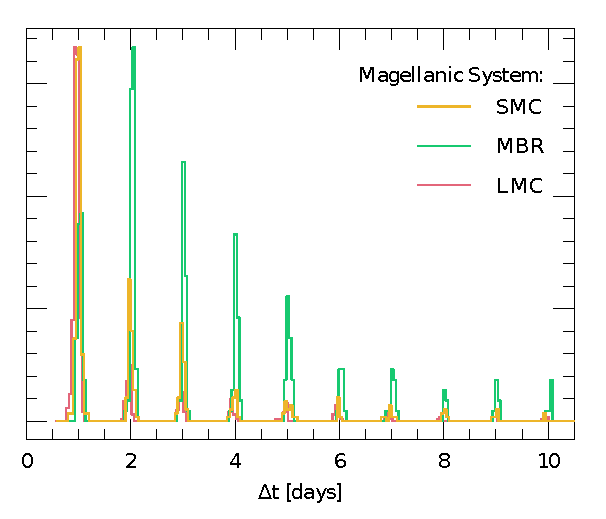
\includegraphics[width=0.45\textwidth]{img/fig_19_65_1_1.pdf}
	\caption[OGLE-IV observation cadence in the Magellanic system]{
		Histogram of the time difference between consecutive observations on OGLE-IV, for the clouds (LMC, SMC) and the Magellanic Bridge (MBR).
		\autoref{fig:1234-cadence} is basically a phase diagram of the LMC histogram, 
		but only considering the observations made to one star.
		The vertical scale is normalized to the highest point of each curve.
		Taken from \cite{OGLE2015}, Figure 19.
	}
	\label{fig:global-cadence}
\end{figure}

\section{Implementation details}

All of the algorithms presented here are programmed in Python \citep{VanRossum2009} for simplicity,
but with extensive use of the NumPy \citep{vanderWalt2011} and Numba \citep{Lam2015} libraries to achieve greater performance.

No claim is made that these algorithms are optimal, 
but effort was putted on implement the optimizations commonly used in the literature.

All of the algorithms take a time array, a magnitude array, and a frequency array as parameters.
The minimum entropy and minimum dispersion algorithms also take an integer number of bins.

\subsection{Algorithms}

\subsubsection{Arclength}

For each frequency in the search array:

\begin{itemize}
	\item \autoref{lst:phase} is used to calculate the phase with the time and magnitude arrays.
	\item The phase array is sorted, and the magnitude array is rearranged accordingly.
	\item The differences between contiguous phases and magnitudes are calculated.
	\item Those differences are squared and then added, according to \autoref{eq:arclength}
	\item Optionally, the square root is taken. This does not affect the peaks except by a scaling.
	\item The total sum is returned as the arclength.
\end{itemize}

The best guess for the correct frequency would be where the arclength is minimum.
A possible implementation of a single iteration of the method is given in \autoref{lst:arclength}.

\subsubsection{Entropy}

For each frequency in the search array:

\begin{itemize}
	\item \autoref{lst:phase} is used to calculate the phase.
	\item A binning algorithm, like \autoref{lst:hist2d}, is used to calculate a 2D histogram of the phase diagram.
	\item The histogram counts are transformed in the probabilities $\mu_j$ of \autoref{eq:entropy}.
	\item The zero probability bins are deleted, to avoid a numerical error taking the logarithm.
	\item The sum on \autoref{eq:entropy} is returned as the entropy.
\end{itemize}

The best guess for the correct frequency would be where the entropy is minimum.
A possible implementation of an iteration is given in \autoref{lst:entropy}.

A big improvement can be made by translating the phase-magnitude plane $\{\phi_k,m_k\}$ into a line $\lfloor m_k n_{bins} \rfloor + \phi_k$,
analogous at making the phase \enquote{decens} and the phase \enquote{units}.
Over that transformed line, a 1D histogram algorithm can be used with $n_{bins}^2$ number of bins, hence the phase diagram is \enquote{flattened}. 
That implementation is given in \autoref{lst:entropy-flattened}. 
This flattening allows the use of very efficient 1D binning algorithms.

\subsubsection{Dispersion}

For each frequency in the search array:
\begin{itemize}
	\item \autoref{lst:phase} is used to calculate the phase.
	\item For each uniform zone (partition of the phase $[0,1]$ range), 
	calculate the occupation number and the variance of the magnitudes corresponding to the phases on the zone.
	\begin{itemize}
		\item If the zone is empty, the variance is defined as zero. This makes some sense because the (biased) variance 
		$\frac{\sum(x-\bar{x})^2}{n}$ would be an empty sum with a second order zero in the numerator and a first order zero in the denominator.
	\end{itemize}
	\item The pooled variance $s^2$ of all the zones is calculated with \autoref{eq:pooled-variance}. 
	The overall variance $\sigma^2$ is just the variance of all the magnitudes.
	\item The coefficient of determination $R^2=1-s^2/\sigma^2$ is returned as the dispersion.
\end{itemize}

The best guess for the correct frequency would be where this $R^2$ is maximum.
This $R^2$ approximates really well the Fourier spectrum, as can be seen in \autoref{fig:examples}.
The implementation is in \autoref{lst:dispersion}

\subsubsection{Lomb-Scargle}


The original formulas for the Lomb-Scargle periodogram (Equations \ref{eq:lomb-scargle} and \ref{eq:tau}) 
involve several redundant trigonometric calculations.
Here we implement the optimizations given by \cite{Townsend2010}, where no trigonometric function is repeated.

For each frequency $\nu$ in the search array, being $t$ the time array and $m$ the magnitude array:
\begin{itemize}
	\item Calculate:
	\begin{itemize}
		\item $\omega t = 2\pi\nu t$
		\item $C=\cos\omega t$
		\item $S=\sin\omega t$
		\item $mC= m \cdot C$
		\item $mS = m \cdot S$ 
		\item $CC=C\cdot C$
		\item $SS=S\cdot S$
		\item $CS=C \cdot S$
		\item $\omega\tau = \frac12 \arctan\left(\frac{2 CS}{CC-SS}\right)$
		\item $c_\tau = \cos\omega\tau$
		\item $s_\tau = \sin\omega\tau$
	\end{itemize}
	\item return the coefficient of determination
	$$
	R^2 = \frac12 \left(\frac{(c_\tau mC + s_\tau mS)^2}{c_\tau^2 CC + 2 c_\tau s_\tau CS + s_\tau^2 SS}
	+ \frac{(c_\tau mS-s_\tau mC)^2}{c_\tau^2 SS + 2 c_\tau s_\tau CS + s_\tau^2 CC}\right)
	$$
\end{itemize}

As before, the correct frequency is at maximum $R^2$, and this is also a good approximation of the Fourier spectrum.

\subsubsection{Fourier}

A straightforward calculation of \autoref{eq:fourier} would actually be enough to outperform some (if not all) of the aforementioned methods,
but there is an iterative optimization provided by \cite{Kurtz1985}, that calculates the transform on the next frequency modifying the last calculation,
saving a lot of time.

Thus, contrary to all the other methods, this implementation cannot be putted into a single-iteration function.
Also contrary to the other methods, it requires the frequency grid to be evenly spaced. This is not a problem, 
as the only problem were the \textit{times} to be unevenly spaced.
Additionally, if we have no idea of the correct frequency in the first place, 
there is no worse nor better way to search for it than in an evenly spaced frequency grid.

The idea behind this optimization is that if the frequencies are of the form $\nu_j = \nu_{j-1} + \Delta \nu$, the centroid from \autoref{eq:centroid} 
can be written (element-wise) as

\begin{equation}
	C(\nu_j)_k = f_k e^{2i\pi (\nu_{j-1}+\Delta \nu) t_k} = f_k e^{2i\pi \nu_{j-1} t_k} e^{2i\pi \Delta \nu t_k} = C(\nu_{j-1})_k e^{2i\pi \Delta \nu t_k}
\end{equation}
Where $j$ goes over the frequencies and $k$ over times/magnitudes. 
The array $D_k = e^{2i\pi \Delta \nu t_k}$ is constant, 
so the coordinates of the \enquote{curled object} in the complex plane that we took the centroid off (see \autoref{fig:complex-phase-off})
for a certain frequency, can be calculated from the last coordinates by just multiplying element-wise by $D$.

Given $\nu_0,\nu_f,\Delta \nu$, the time array $t_k$ and the magnitude array $f_k$, the algorithm would look like:

\begin{enumerate}
	\item Calculate $D_k = e^{2i\pi \Delta \nu t_k}$
	\item Allocate an array $F_k$ of the same size as the frequency range, $J=\lfloor \frac{\nu_f-\nu_0}{\Delta \nu} \rfloor$, to store the centroid magnitudes.
	\item Initialize $\nu=\nu_0$.
	\item Calculate the first \enquote{curled object} in the complex plane, $C_k = f_k e^{2i\pi \nu_0 t_k}$.
	\item Initialize $F_0 = \left|\sum_k C_k\right|^2$
	\item While $\nu<\nu_f$, or equivalently, for $j \in [1,J]$
	\begin{itemize}
		\item $C_k \to C_k \star D_k $, where $\star$ means element-wise multiplication
		\item $F_j \to \left|\sum_k C_k\right|^2$
	\end{itemize}
	\item Return $\nu_k = \nu_0 + k \Delta \nu$ where $F_k$ is maximum. 
\end{enumerate}

Perhaps the code on \autoref{lst:fourier} would be clearer.

\subsection{Examples and the sampling problem}

A simple benchmark of the algorithms can be seen on \autoref{fig:runtimes}. 
It is of note that the minimum entropy algorithm (on the naive implementation) was the slowest, 
and the simple Fourier method was the fastest by far, even without optimizations.
The \enquote{flattened} implementation of minimum entropy (on red) is faster than de dispersion one, because the $M^2$ term in the 
$O(nM^2)$ complexity of the entropy calculation is generally small, and there is no linear term on counting bins in the histogram.
On the other side, despite the $O(nM)$ complexity of the dispersion method, each iteration contains variances and counting in addition to the tally,
so there is linear overhead on $n$.
The full spectrum iterative Fourier method has complexity $O(nf)$, with $f$ the number of frequencies.
It is slower than the $O(n \ln n)$, as for our purposes $f\gg n$.
Even with this, the incremental Fourier method seems to be the fastest on uneven sampled data.

Examples of the spectra produced by each method are in \autoref{fig:examples}.
As expected, the Lomb-Scargle and dispersion spectra are very good approximations of the pure Fourier one.
Of course, there are some random noise and minor peaks that make those three differ, and even more with the arclength spectrum.
The entropy spectrum is the most different, considering that the peak is sharper 
(in the first star) and it present false peaks at $\nu\approx 1$/day\footnote{
	It's never exactly 1/day, because of the peak on \autoref{fig:1234-cadence}. 
	The earth moves around the sun, and optimal observing times also move.
	Then the peak will not be exactly at zero.
}. In fact, the Fourier methods also present that peaks, but they can be eliminated.

\begin{figure}
	\centering
	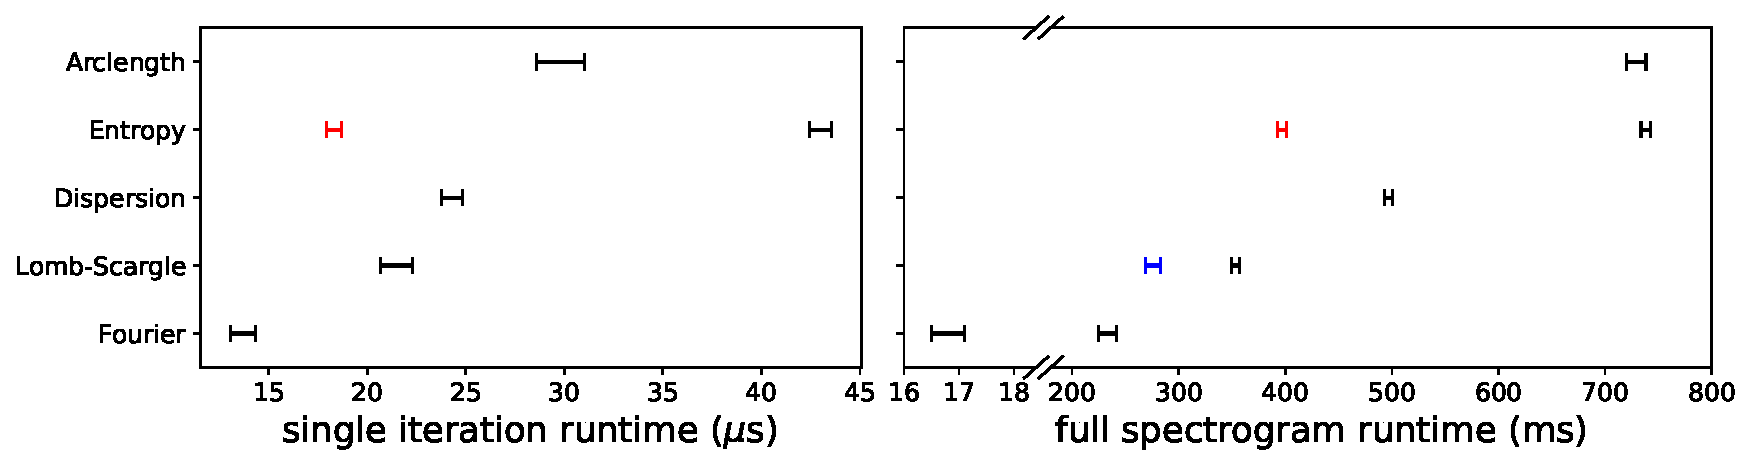
\includegraphics[width=\textwidth]{img/runtimes.pdf}
	\caption[Illustrative benchmark for the algorithms]{
		Sample benchmark of repeated single-threaded runs over all the algorithms described in this section.
		The single iteration times were calculated with 50000 repetitions of 7 runs, 
		and the full spectrum times were made on a regular frequency grid of size 14000, with 10 repetitions.
		The red points of the entropy method refer to the flattened implementation on \autoref{lst:entropy-flattened},
		and the black one to the naive implementation.
		For the Lomb-Scargle method, a blue point with the times for the \texttt{scipy.signal.lombscargle} implementation was given as a reference value.
		The full spectrum time axis is broken to show the difference between the incremental method (\autoref{lst:fourier}) and the simple method (\autoref{lst:fourier-single}).
		The machine used was a domestic computer with Intel \textregistered{} Core$^{\text{TM}}$ i7-4702MQ CPU @ 2.20GHz.
	}
	\label{fig:runtimes}
\end{figure}

This peaks are a common occurrence, because of the near-nightly cadence of the data acquisition process (see \autoref{fig:global-cadence}).
We can take a closer look at the phase diagram and Fourier curling on one of those false peaks in \autoref{fig:problem}.

\begin{figure}
	\centering
	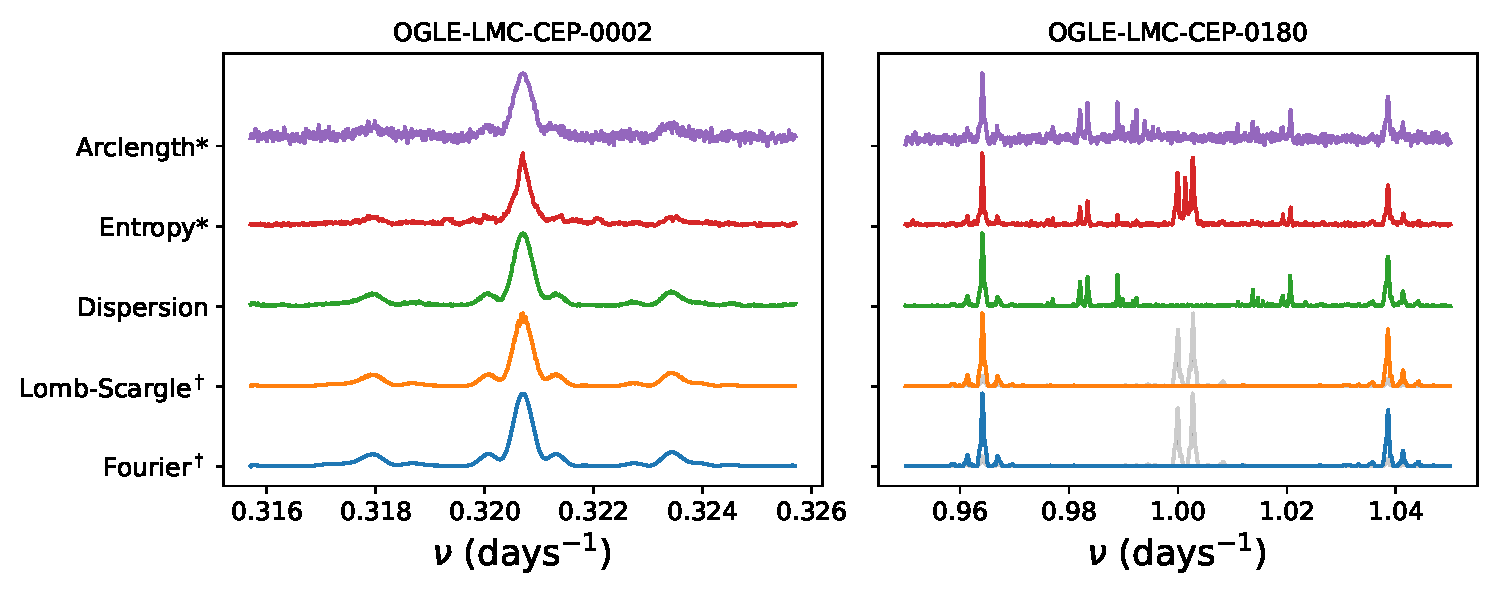
\includegraphics[width=0.99\textwidth]{img/examples.pdf}
	\caption[Example of spectra near the true frequency]{
		Sample spectra for the five methods described in this section, for two different stars, neasr the true frequency.
		$(\ast)$: Arclength and Entropy spectra were inverted to allow direct comparison with the Fourier approximations.
		$(\dagger)$: The Fourier, Lomb-Scargle and entropy methods present a false peak (in light gray) 
		when the frequency is very near 1/day; see text for details.
	}
	\label{fig:examples}
\end{figure}

\begin{figure}
	\centering
	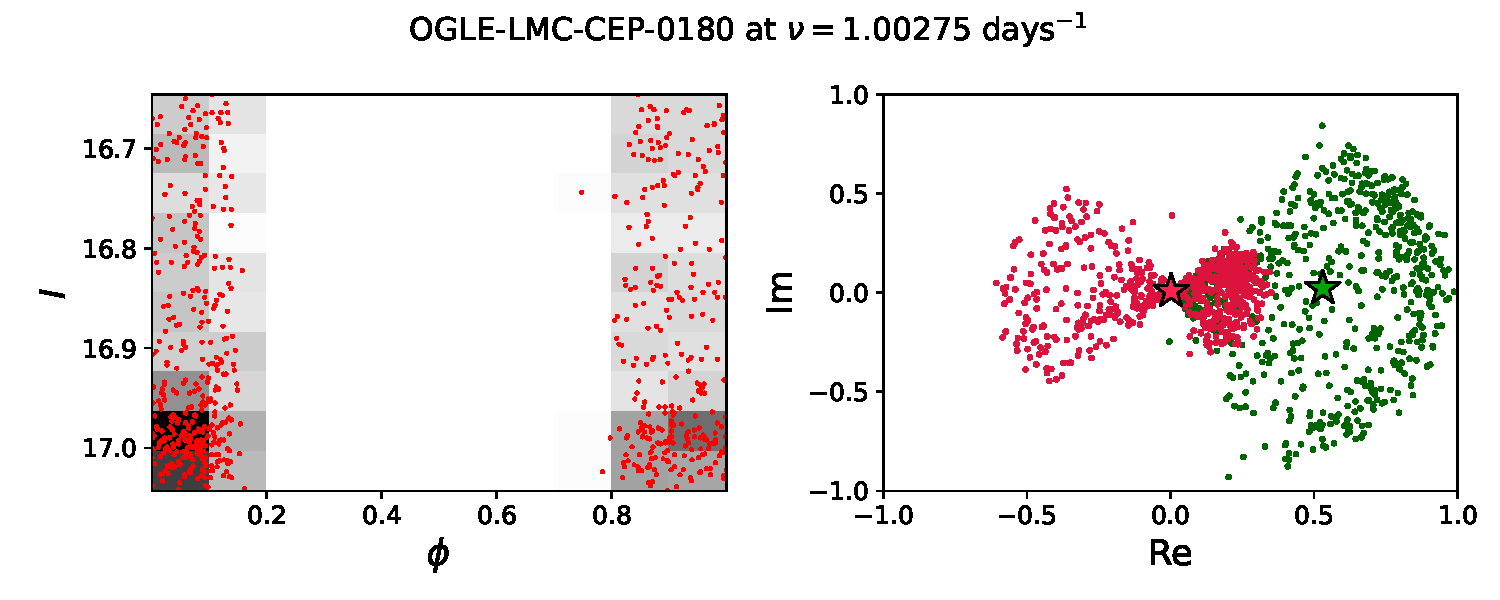
\includegraphics[width=0.99\textwidth]{img/alias.pdf}
	\caption[Detail of the failure mode of Fourier and entropy methods]{
		Detail of the phase diagram and complex phase curling of the star from \autoref{fig:examples}, very near the false peak at 1.00275/day.
		The histogram was made with 10 bins on each axis.
		The green and magenta dots represent a Fourier curling where the magnitude has been normalized in the respective intervals 
		$[0,\text{max}-\text{min}]$ and $[\text{min}-\text{mean},\text{max}-\text{mean}]$ (such that the mean becomes zero).
		The big stars lie on the centroid.
	}
	\label{fig:problem}
\end{figure}

Then is suddenly clear why the entropy method fails: the dots are distributed phase-wise in a similar fashion as in \autoref{fig:1234-cadence}.
That leaves a huge gap (in this case in the middle), and if there are many bins with probability zero the entropy would certainly be lower,
because it is more ordered that way; there are chunks of the phase diagram histogram that are uniform, and therefore the entropy method gives a false positive.

Something similar happens with the curled figure in the complex plane. As each point is rotated almost $360^\circ$ 
(again, how much more or less than that is dictated by \autoref{fig:1234-cadence}), and if the radii are all positive that means the centroid would be near the positive reals.
There is a simple solution: make the mean radius zero. That way, the negative radius would end in the $180^\circ$ side of the complex plane, and everything would cancel nicely.

\autoref{fig:problem} also allow us to understand how the arclength and dispersion spectra are \enquote{immune} to this effect. 
If we connect the dots of the phase diagram,  at least one line should join the two groups, and it will be a big line.
So no matter how close get those points on the sides, the big line between them should carry the weight of this strange alignment.
That works until everything aligns in one clump in the middle, and suddenly there is no line. This behavior deserves further study.
On the other side, we defined the empty variance as zero. 
Therefore the terms corresponding at the empty gaps would just not contribute, neither in the denominator nor in the numerator of \autoref{eq:pooled-variance}.
It would be as if someone had just cut out the empty columns. The rest is just vertical chaos, having in fact maximal variance,
so the dispersion method is truly immune with our definitions.
 






%\section{Pulsation mode determination}



\chapter{Results}

\section{Data preparation and periodogram calculation}

All the classical Cepheid data from the OGLE download site was downloaded using an script (\autoref{lst:download})
designed to replicate the folder tree of the site, for better programmatic access to the data.
The downloaded files amount to $\sim$47 MB.

Next, the pandas library \citep{pandas} was used to perform the statistical analysis shown on \autoref{sec:data}.
Accordingly to the stated there, only the $I$ magnitude data was used to search for the period.

Following the sample benchmark done on \autoref{fig:runtimes}, 
the incremental implementation of the Fourier periodogram (\autoref{lst:fourier}) was selected to find the period of each star with $I$ magnitude data.
A linear frequency grid was used to calculate the periodogram, starting from $\nu_0=0.001$/day ($P= 1000$ days), 
incrementing on steps of $d\nu = 10^{-5}$/day, up to $\nu_f=4.7$/day ($P=0.212$ days), giving a total of 469900 test frequencies, 
99000 of which are in the $(1,100)$ days period range.
With a modification on the implementation, an linear period grid could be used instead with the incremental transform.
The ideal grid would be linear on $\log P$, as that is the variable in which the PL relation is linear; 
however, the faster incremental implementation cannot be used on an uneven grid, and so the slower Lomb-Scargle or simple Fourier periodogram must be used instead.

As deduced in \autoref{sec:examples-and-aliases}, 
the magnitude data was normalized to zero mean to prevent finding false peaks caused by the near-periodic cadence of the data.
After that, each periodogram was calculated, and normalized to the principal (highest) peak.
A peak detection algorithm by SciPy \citep{scipy} was used to capture the secondary peaks which height were greater than half the principal peak.
This was motivated by the intuition that if a spectrum has many high peaks, 
the true frequency would be uncertain, and that could be later used as a criterion to clean the PL diagram from outliers.
The peak widths at half maximum were calculated, as this is the only measure of the uncertainty of the found frequency at our disposal.
This frequency uncertainties were never greater than 0.0014/day.

After every star on each Cloud (with $I$ and $V$ data) have passed through this process, the results were saved in one structured data file, in this case in the \texttt{JSON} format.
The number of detected peaks on the spectrum, compared to the number of data points available for each star, can be found in \autoref{fig:peaks-n-points}.
Limits to the number of detected peaks and data points were decided to eliminate outliers from the next step, which is the PL relation.

\begin{figure}
	\centering
	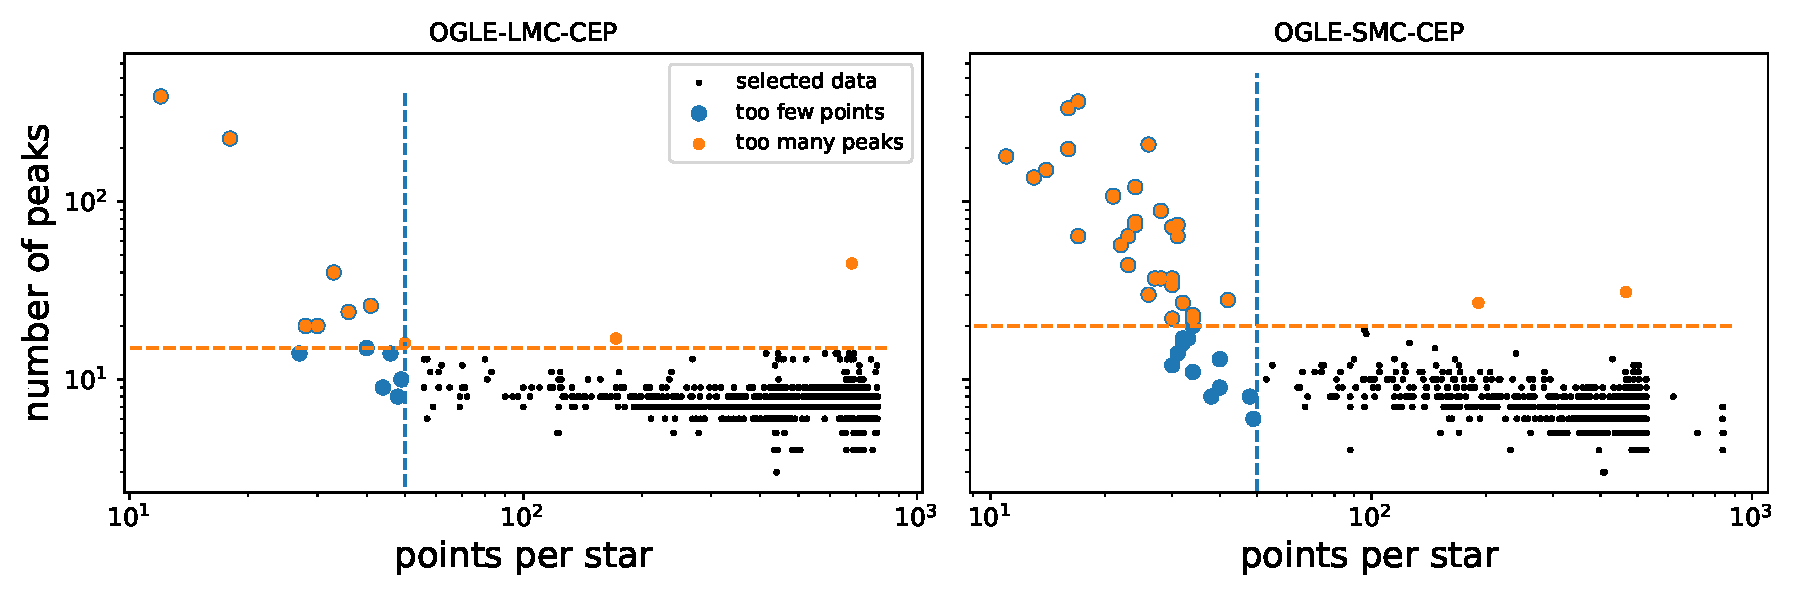
\includegraphics[width=0.9\textwidth]{img/peaks_vs_points.pdf}
	\caption[Results: detected number of peaks against data size]{
		Detected number of peaks plotted against the size of the data for each Cepheid in the Magellanic Clouds.
		The stars with less than 50 points were considered to have too little data to conclude that the frequency found with the algorithm is indeed the correct one.
		The same doubt is casted on those stars with a high number of peaks in the spectrum. The limit is 15 peaks for the LMC and 20 for the SMC.
		Those limits were chosen to maximize the number of outliers discarded from the PL relation (\autoref{fig:pl-result}) without discarding seemingly good placed stars in the PL diagram.
		This leaves 4341 stars in the LMC and 4655 in the SMC.
	}
	\label{fig:peaks-n-points}
\end{figure}


\autoref{eq:wesenheit-i} was used to calculate the extinction-free Wesenheit index, 
with $R_I=1.55$ \citep{OGLE2015,Ulaczyk2013} and the mean $I$ and $V$ magnitude for each one of the 8996 remaining stars.
Uncertainty in the mean of each magnitude was also computed, using contribution from two factors.
The first was compound uncertainty, using the errors reported for each magnitude measurement, calculated as $1/\sigma_{total}=\sqrt{\sum_i 1/\sigma_i^2}$.
The second factor was estimated via bootstrap, as the standard deviation of the mean from several resampling of the magnitudes.
The resulting uncertainties were never greater than 0.04 mag, for the selected data. 
The distribution of uncertainties is plotted on \autoref{fig:uncertainties}, 
and its corresponding error bars on the PL diagram would be barely even visible.

\begin{figure}
	\centering
	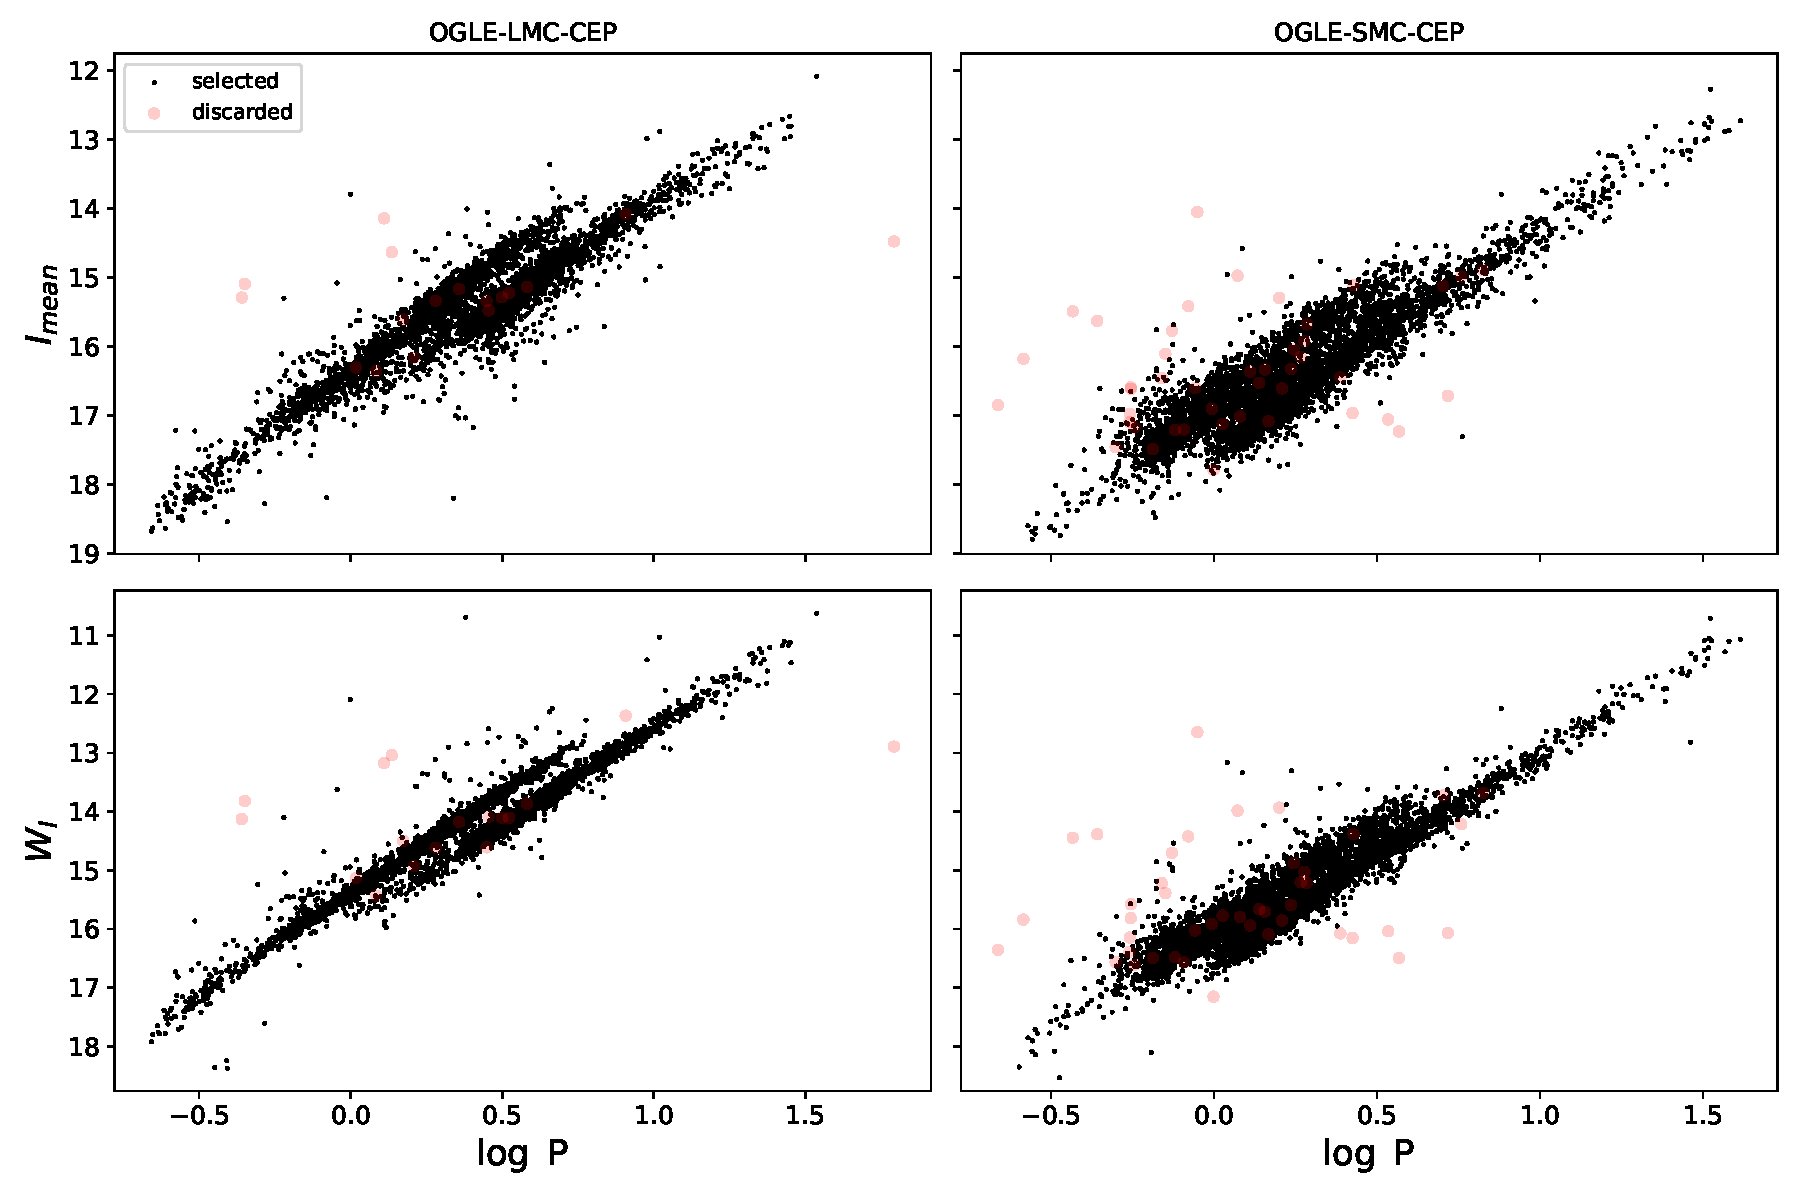
\includegraphics[width=\textwidth]{img/PL_realtion.pdf}
	\caption[Results: PL relation for the Magellanic Clouds]{
		Period-Luminosity diagrams for classical Cepheids int he Magellanic Clouds, on $I$ magnitude and $W_I$ index.
		Discarded stars according to the criteria presented in \autoref{fig:peaks-n-points} are shown as faint red shadows.
		In each diagram, two main linear tendencies can be noted, the fundamental and the first overtone tendencies.
		It is notable how well the Wesenheit index separates the two tendencies, especially in the LMC.
	}
	\label{fig:pl-result}
\end{figure}

\section{PL relations for the Magellanic Clouds}

If we plot the Wesenheit index against the frequencies of the highest peak for each star, remembering that $\log P=-\log \nu$, we obtain \autoref{fig:pl-result},
the Period-Luminosity relation for the Magellanic Clouds. This is a good reproduction of the results from \cite{OGLE2016}, 
from where we can associate the lower linear tendency to the \texttt{F} pulsation mode and the upper one with the \texttt{1O} mode, or the first overtone.
Some few stars of the \texttt{2O} mode can be observed at the back of the \texttt{1O} tendency, around $\log P\approx 0$.
This is of course just a general association, given that we did not perform pulsation mode analysis on these results.
Also, multimode pulsators like \texttt{F1O} or \texttt{1O2O} cannot be separated from their lowest frequency on this kind of PL diagram.

The Wesenheit index is as successful as expected on reducing the dispersion on the diagram.
This method is just a mean approximation of the reddening, and as such, it is limited, but great separation is achieved on the LMC diagram.
The dispersion, however, is far grater in the SMC compared to the LMC. 
Despite this specific dataset having fewer points per star in the SMC, this should not be an artifact of the data, 
but a result of the SMC being farther away than the LMC, at $62.44 \pm_{stat} 0.47 \pm_{sys}0.81$ kpc 
and $49.97 \pm_{stat} 0.19 \pm_{sys} 1.11$ kpc respectively \citep{SMC2020,LMC2013}.

\subsection{Comparison with OGLE-IV results}


Some disperse points in the PL diagram were also present in the OGLE results. 
Those stars could be just missclassified, something that occurs fairly often \citep[see for example Table 1 of][]{OGLE2016};
some stars previously thought to be classical Cepheids turned out to be of the RR Lyr\ae{} class,
or anomalous Cepheids, or even Eclipsing variables.

Our results, however, are not in perfect agreement with those of \cite{OGLE2016}.
Several outliers can be seen in the diagrams presented here, but some of those are also in the OGLE-IV results.
Fortunately, in the download site there are several \texttt{*.cep} files that contain the periods found by them.
Using that data, we can directly compare the results, information presented in \autoref{fig:comparison}.

\begin{figure}
	\centering
	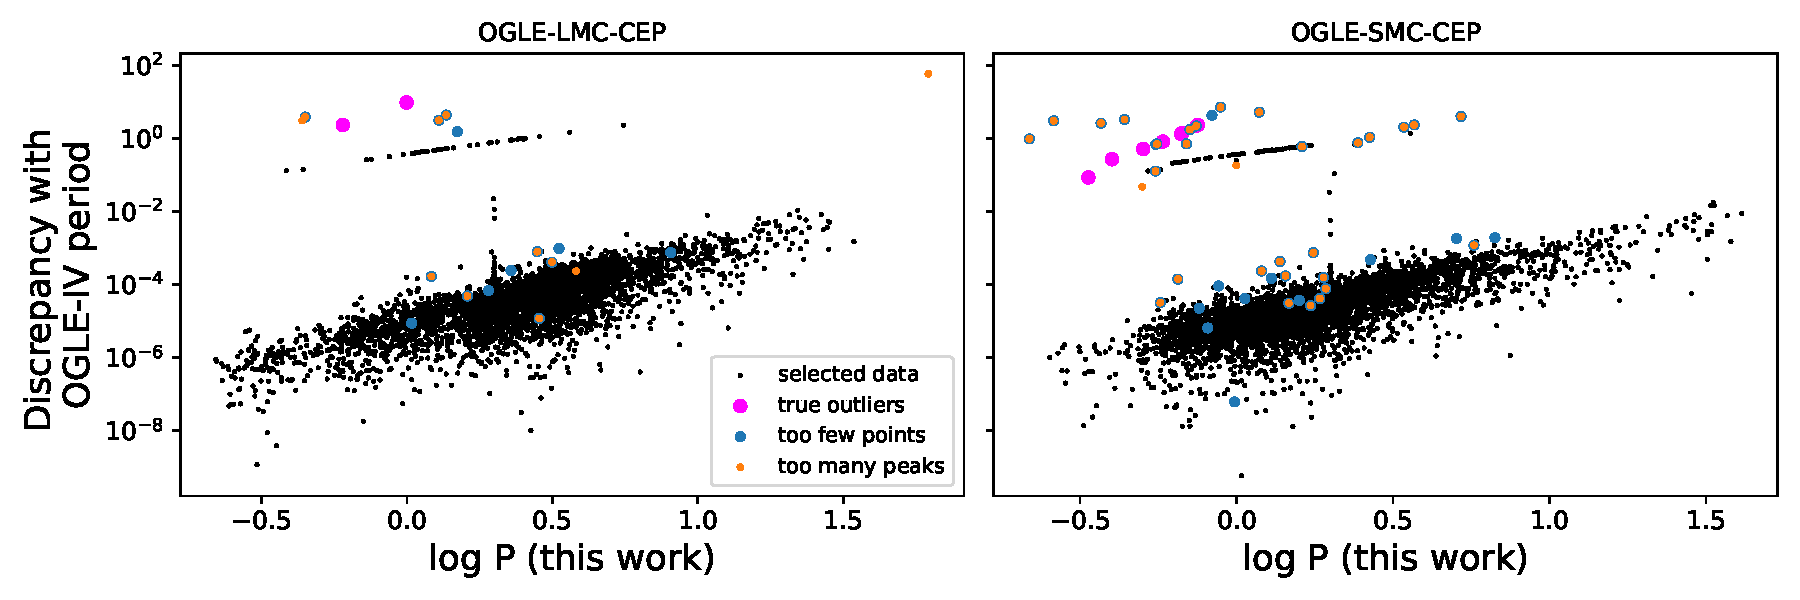
\includegraphics[width=0.95\textwidth]{img/discrepancies.pdf}
	\caption[Results: comparison with OGLE-IV periods]{
		Absolute differences between the periods found on this work and those found on the OGLE data site, as a function of $\log P$.
		Five groups can be discerned: (1): the bulk of stars, those in accordance to the OGLE period, shown in black. 
		(2): a tiny subset of those, forming a near vertical line of increasing discrepancy, at around  $\log P = 0.3$, and connects with
		(3): a thin horizontal line of stars with discrepancy of about 0.1 to 1.
		(3) and (4): the points excluded from the PL relation since \autoref{fig:peaks-n-points}, on blue and orange.
		(5): the remaining points with high error after removing (2-4), denominated \enquote{true outliers}, shown in magenta.
	}
	\label{fig:comparison}
\end{figure}

The majority of stars are located in the low discrepancy side of that diagram, which means there are general agreement with the OGLE results;
98\% of the stars with both $I$ and $V$ data were found in this work to have a period that did not differ from the OGLE period more than $0.01$ days.
In the LMC there were 51 stars with a discrepancy greater than 0.01 days, and 84 in the SMC.

A general trend can be observed: the discrepancy is larger the larger the period.
This suggest that a period grid, not a frequency one, was used to produce th OGLE results.

\begin{figure}
	\centering
	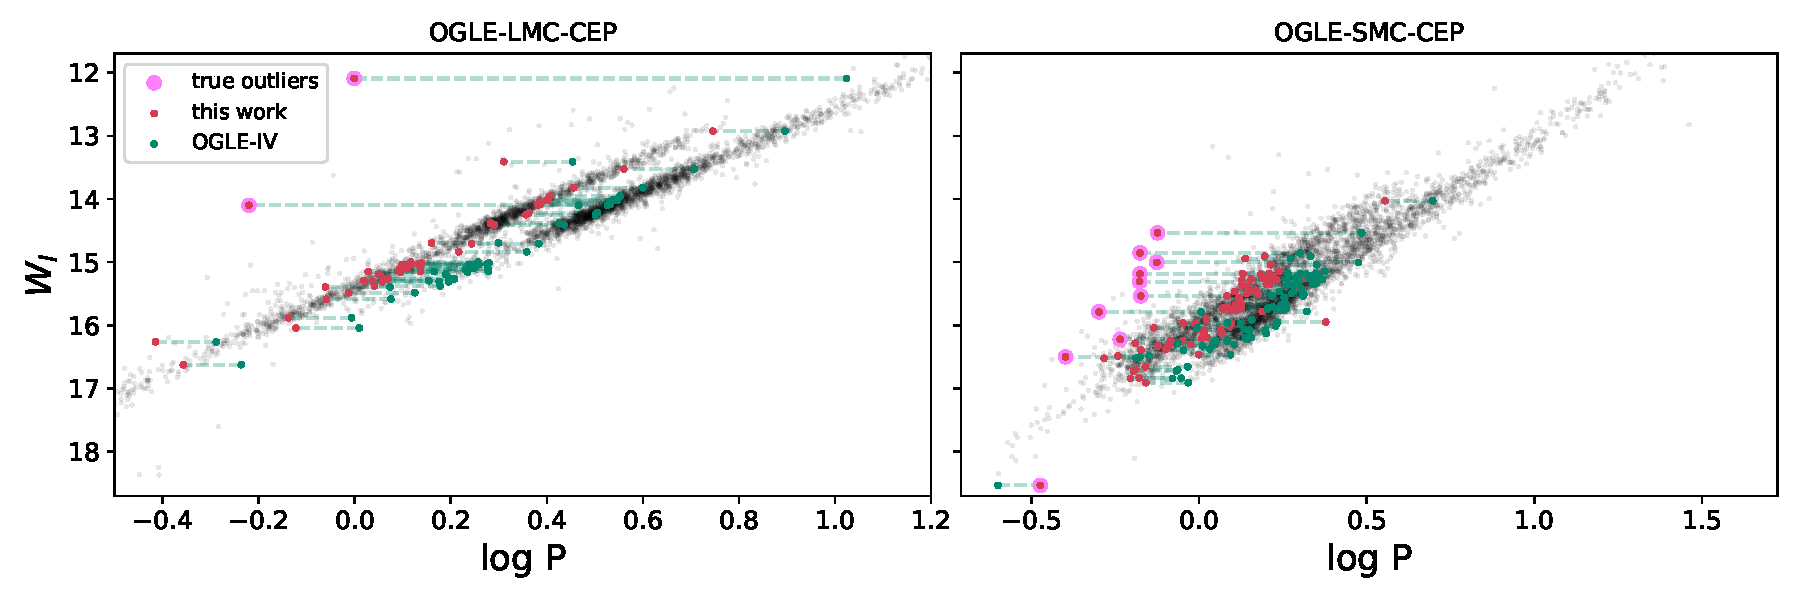
\includegraphics[width=\textwidth]{img/horizontal_line_corrections.pdf}
	\caption[Results: comparison with OGLE-IV periods]{
		Differences on period for the horizontal line (3) from \autoref{fig:comparison} and true outliers (5), when using the period found in this work (on red)
		and the displacement  (green dashed line) to their positions when using the periods from OGLE (on green).
		Big magenta circles are drawn on the true outliers from  \autoref{fig:comparison}.
	}
	\label{fig:horizontal-line-corrections}
\end{figure}

\subsubsection{The horizontal line}

But there is a more interesting feature in that graphic: a very thin line of stars with discrepancy larger than 0.02, 
too well organized to be the result of few data points or poor random sampling.
The effect is clearly systematic, yet no a priori way of isolating this line from the data was found.
Manually selecting this region in \autoref{fig:comparison}, 
we could track their $\log P$ movement in the PL diagram if we use our periods and OGLE's.
That is plotted in \autoref{fig:horizontal-line-corrections}.
Almost all of those stars are in the \texttt{1O} tendency when using the periods found on this work,
and pass to the \texttt{F} tendency when using the periods from OGLE. 

With that information one could suspect that these were multimode \texttt{F1O} Cepheids 
that our algorithm just happened to found by their first overtone frequency rather than their fundamental one.
A reverse search in the OGLE classification files for the code of these stars confirms that, indeed, 
of the 45 stars on the horizontal discrepancy line of the LMC, 44 of them were classified as \texttt{F1O} pulsators.
The remaining star, code \texttt{1378}, was a \texttt{F1O2O} multimode, so in fact the argument holds.
For the SMC case, there were 69 stars on the line, with 63 of them being \texttt{F1O} pulsators.
Here the correlation ends, as the remaining six were four fundamental (\texttt{0473},\texttt{1029},\texttt{2792},\texttt{4675}) 
and two \texttt{1O2O} ones (\texttt{0998}, \texttt{4784}).
By better analyzing the overtone content of these stars, 
their pulsation modes could be taken into account to place them in the proper side of the PL tendencies,
eliminating the systematic line of \autoref{fig:comparison}.

\subsubsection{The vertical line}

The next thing that jumps into view from \autoref{fig:comparison} is the tiny bridge 
that connects the low error results with the horizontal line (2).
A detailed plot of those points can be seen in \autoref{fig:vertical-discrepancy}. 
On the selected range, which is somewhat arbitrary on the low error side, there are 13 stars for the LMC and 12 on the SMC.
Most of those stars are \texttt{1O} pulsators for the LMC and \texttt{F} pulsators for the SMC, 
and they are placed in between of the two tendencies of the PL diagram, so the missclassification argument presented above does not hold.
Like before, no a priori way of detecting these stars was found.

\subsubsection{The true outliers}

The magenta dots on \autoref{fig:horizontal-line-corrections} represent the true outliers, 
those few for which the period found in this work differ significantly from the OGLE period,
despite having a typical number of data points and also a typical number of peaks in their spectrum.
This could mean that the algorithm simply failed, either because some irregularity on the data or in the implementation. 

The two outliers of the LMC have OGLE codes \texttt{0016} and \texttt{4668}, and are fundamental pulsators according to OGLE.
The 10 SMC ones have codes 
\texttt{1400}, 
\texttt{2521}, 
\texttt{2924}, 
\texttt{3108}, 
\texttt{4020}, 
\texttt{4361}, and
\texttt{4967} (fundamental pulsators);
\texttt{3317} and
\texttt{4195} (\texttt{1O} pulsators); and 
\texttt{1350} (\texttt{1O2O} pulsator).

\subsection{Secondary peaks in the PL diagram}

A diminished reflection of the spectrum near integer frequencies was found for nearly all individual stars,
as the blue spectrum illustrated in \autoref{fig:uneven-advantage}.
That resulted on the secondary peaks of each star spectrum to form patterns around those points of integer frequencies.

Some of the frequencies found for some stars lied on that secondary peak zone, indicating that they were not the optimal period for that star.
This can possibly be solved by refining the search around all the peaks found above the noise of the spectrum.
As can be seen in \autoref{fig:peaks-n-points}, the number of peaks is of the order of $\sim20$ or less for stars with a reasonable amount of data,
so this additional search with a finer grid, perhaps in the interval $[\nu_{peak}-\,d\nu,\nu_{peak}+\,d\nu]$, should not take too much of additional processor time,
and can be performed using any of the algorithms discussed in this work, as false peaks have been eliminated in the first run.

A PL diagram on linear frequency of these secondary peaks, demonstrating the analogy with \autoref{fig:uneven-advantage}, is presented on \autoref{fig:linear-color-pl-lmc}.
Versions of \autoref{fig:pl-result} with those same secondary peaks for both Clouds are in \autoref{fig:color-pl-lmc} and \autoref{fig:color-pl-smc},
where the misplaced principal peaks of the outliers can be seen lying with the secondary peaks.


% additional peaks diagrams on the appendix
% those true outliers are positioned in the second peak of the spectrum in the colorful figures
%some yellow dots can be seen lying around the secondary peaks. This can possibly be resolved by searching with a fined $d\tau$ around each founded peak, 
% to find the true maximum of each one. This can be done with any of the five algorithms, as the speed should not be a problem for so few points.

\chapter{Conclusions and Future Work}

%The OGLE PL relations on the Magellanic clouds were reproduced with a simple implementation of the Fourier periodogram, 
%and two tendencies were observed for the fundamental and first overtone pulsation modes.
%Those two tendencies are more clearly separated when using the mean extinction-free Wesenhit index on the magnitude axis,
%but in both cases the LMC data showed less dispersion from the linear tendency than the SMC data.
%
%Outside the periods corresponding to an integer number of days, all the methods here presented provide good approximations to the pulsation spectrum of a star.
%These problematic points on the period line are caused by the near-periodic observation cadence (fig),
%and normalization methods were presented for eliminating these problematic alias peaks on the Fourier, Lomb-Scargle, and dispersion periodograms.
%The arclength periodogram naturally evades this problem, whereas no solution to this problem could be found for the entropy spectrogram.
%
%Python routines implementing the five periodograms were presented, 
%and the acceleration provided by Numba makes them useful for signal analysis work.

%The uneven sampling was proven a key feature of the data. If measurements had been taken at a cadence of exactly one day,
%we could not have searched for any period of less than one day, because the periodogram would reflect at each half per day requency, the Nyquist frequency.
%Therefore, the PL relation would have been limited at $\log P>0$, which cuts in half the first overtone tendency.




\section{Future work}


%* Individual dereddening R_I wesenheit index
%* Pulsation modes without fitting a Fourier series: that information must already be in the spectrum
%	* The phase is lost when conjugating in (EQUATION), which all method implicitly do except fot the pure Fourier one. For example, in (LISTING single it fourier) the "phase spectum" could be obtained by returning the complex argument of the centroid, and not just its magnitude
%* Find a way to correct the alias peaks on the entropy periodogram



% reddening maps: per star wsenheit index

% time dependence of amplitude and pulsation period and overtones
	% stellar evolution, blue loops

% multi period stars

% abnormaly long period cepheids (Araucaria Project)

% non linearity and robust regression for the PL relation

% Bibliography

\bibliographystyle{aa} % style aa.bst
\bibliography{global.bib}

% Appendices

\appendix
\appendixpage
\noappendicestocpagenum
\addappheadtotoc

\chapter{Code utilities}
\section{C listings}


\begin{listing}[H]
	\begin{minted}{c}
	double eps(double x) {
	    long i = *(long*) &x;
	    i++;
	    double x_next = *(double*) &i;
	    return x_next - x;
	}
	\end{minted}
	\caption[\texttt{eps} C function]{
		C code of a function that estimates the machine epsilon for a given double precision floating point: 
		the minimum value for which $x+\epsilon/2 > x$ still holds.
		This code exploits the fact that consecutive floating point numbers must have consecutive bit representations.
	}
	\label{lst:c-eps}
\end{listing}



\section{Python listings}

For all the code fragments in this section, \autoref{lst:python-header} 
is used to define the names of the NumPy and Numba package namespaces.
The Numba notation for function signatures is given on \autoref{tab:numba-types}.
A string using these types in the \texttt{njit} decorator is given to allow ahead-of-time compilation.
The notation for these strings is \texttt{return\_type(arg1\_type,arg2\_type,...)}.

\begin{table}
	\centering
	\begin{tabular}{r|l}
		Type & notation \\\hline\hline
		64 bit float & \texttt{f8} \\
		64 bit signed integer & \texttt{i8} \\
		Contiguous 1D array & \texttt{f8[::1]} \\
		Row-contiguous 2D array & \texttt{f8[:,::1]} 
	\end{tabular}
	\caption[Numba type aliases]{
		Numba types used in the code for this work. 
		The full list can be consulted on \url{https://numba.pydata.org/numba-doc/dev/reference/types.html}
	}
	\label{tab:numba-types}
\end{table}

\begin{listing}
	\begin{minted}{python}
	import numpy as np
	from numba import njit
	\end{minted}
	\caption[Library aliases for Python]{Common library imports for all the Python listings.}
	\label{lst:python-header}
\end{listing}


\begin{listing}
	\begin{minted}{python}
	@njit("f8[::1](f8[::1],f8)")
	def phase(t_arr,f_test):
	    return np.mod(t_arr*f_test,1.0)
	\end{minted}
	\caption[\texttt{phase} function]{
		Straightforward implementation of \ref{eq:phase}. 
		The ephemeris is no included, since it does not matter for any of the algorithms,
		an is used just as a visual aid to present the light curves.
	}
	\label{lst:phase}
\end{listing}

\begin{listing}
	\begin{minted}{python}
	@njit("f8(f8[::1],f8[::1],f8)")
	def arclength(t_arg,m_arg,f_test):
	    phi = phase(t_arg,f_test)
	    index = phi.argsort()
	    return sum(np.diff(phi[index])**2 + np.diff(m_arg[index])**2)
	\end{minted}
	\caption[Arclength method implementation]{
		Here, \texttt{numpy.argsort} (which is implemented as a quicksort) is used to simultaneously 
		sort the phase array and rearrange the magnitude array.
		The phase array is calculated with \autoref{lst:phase}.
	}
	\label{lst:arclength}
\end{listing}

\begin{listing}
	\begin{minted}{python}
	@njit("f8[:,::1](f8[::1],f8[::1],i8)")
	def hist2d(x_arr,y_arr,bins):
	    x = x_arr.copy()*bins
	    y = y_arr.copy()*bins
	    H = np.zeros((bins,bins))
	    for i in range(bins):
	        for j in range(bins):
	            H[i,j] += sum((i<=x)*(x<=i+1)*(j<=y)*(y<=j+1))
	    return H
	\end{minted}
	\caption[2D histogram simple algorithm]{
		A simple algorithm to calculate a 2D histogram. 
		It returns a matrix of shape \texttt{(bins,bins)} showing how many points of the data fall on each bin.
		Both \texttt{x\_arr} and \texttt{y\_arr} are assumed to be normalized on the $[0,1]$ interval, for simplicity.
	}
	\label{lst:hist2d}
\end{listing}

\begin{listing}
	\begin{minted}{python}
	@njit("f8(f8[::1],f8[::1],f8,i8)")
	def entropy(t_arg,m_arg,f_test,bins):
	    phi = phase(t_arg,f_test)
	    H = hist2d(phi,m_arg,bins)
	    mu = H.ravel() / len(phi)
	    mu = mu[np.nonzero(mu)]
	    return -mu@np.log(mu)
	\end{minted}
	\caption[Naive entropy method implementation]{
		Algorithm to calculate the entropy of a phase diagram, 
		avoiding numerical error on large \texttt{bins} by deleting the zero probability zones.
	}
	\label{lst:entropy}
\end{listing}

\begin{listing}
	\begin{minted}{python}
	@njit("f8(f8[::1],f8[::1],f8,i8)")
	def entropy_flattened(t_arg,m_arg,f_test,bins):
	    phi = phase(t_arg,f_test)
	    rounded_mag = np.empty_like(m_arg)
	    np.round(bins*m_arg,0,rounded_mag)
	    counts = np.histogram(phi+rounded_mag,bins=bins**2)[0]
	    mu = counts/len(t_arg)
	    mu = mu[np.nonzero(mu)]
	    return -mu@np.log(mu)
	\end{minted}
	\caption[\enquote{Flattened} entropy method implementation]{
		Algorithm to calculate the entropy of a phase diagram, 
		flattening and rounding the magnitude scale in order to use a 1D histogram algorithm.
	}
	\label{lst:entropy-flattened}
\end{listing}

\begin{listing}
	\begin{minted}{python}
	@njit("f8(f8[::1],f8[::1],f8,i8)")
	def dispersion(t_arg,m_arg,f_test,bins):
	    x = phase(t_arg,f_test)*bins
	    ss = np.zeros(bins) # zone variances
	    n = np.zeros(bins) # zone occupations
	    for i in range(bins):
	        mask = (i<=x)&(x<=i+1)
	        n[i] = mask.sum()
	        if n[i] == 0:
	            ss[i] = 0 # empty variance
	        else:
	            ss[i] = np.var(m_arg[mask])
	    s2 = ((n-1)@ss)/(n-1).sum() # pooled variance
    return 1-s2/np.var(m_arg)
	\end{minted}
	\caption[Dispersion method implementation]{
		Algorithm to calculate the dispersion of a phase diagram.
		There is some resemblance between this code and \autoref{lst:hist2d};
		the \texttt{mask} array effectively takes a 1D histogram of the phase, 
		contrary to a 2D one, and thus its faster.
		Care is taken when taking an empty variance, because it is not defined in NumPy.
	}
	\label{lst:dispersion}
\end{listing}


\begin{listing}
	\begin{minted}{python}
	@njit("f8(f8[::1],f8[::1],f8)")
	def lombscargle(t_arg,m_arg,f_test):
	    omega_t = f_test*2*np.pi*t_arg
	    c = np.cos(omega_t)
	    s = np.sin(omega_t)
	    mc = sum(m_arg*c)
	    ms = sum(m_arg*s)
	    cc = sum(c**2)
	    ss = sum(s**2)
	    cs = sum(c*s)
	    omega_tau = np.arctan(2*cs/(cc-ss))/2
	    c_tau = np.cos(omega_tau)
	    s_tau = np.sin(omega_tau)
	    P = 1/2 * (
	        (c_tau*mc+s_tau*ms)**2/(c_tau**2*cc+2*c_tau*s_tau*cs+s_tau**2*ss) + 
	        (c_tau*ms-s_tau*mc)**2/(c_tau**2*ss+2*c_tau*s_tau*cs+s_tau**2*cc)
	    )
	    return P
	\end{minted}
	\caption[Non-redundant implementation of the Lomb-Scargle periodogram]{
		Non-redundant implementation of the Lomb-Scargle periodogram, according to \cite{Townsend2010}.
		This is similar to the \href{https://github.com/scipy/scipy/blob/master/scipy/signal/\_spectral.py}{SciPy implementation}, 
		but here Numba is used instead of Pythran. 
	}
	\label{lst:lomb-scargle}
\end{listing}

\begin{listing}
	\begin{minted}{python}
	@njit("f8(f8[::1],f8[::1],f8)")
	def fourier(t_arg,m_arg,f_test):
	    return abs(sum(m_arg*np.exp(-2j*np.pi*t_arg*f_test)))**2
	\end{minted}
	\caption[Naive implementation of the Fourier periodogram]{
		Simple implementation of an iteration of the Fourier periodogram, without any optimizations.
	}
	\label{lst:fourier-single}
\end{listing}

\begin{listing}
	\begin{minted}{python}
	@njit("f8[::1](f8[::1],f8[::1],f8,f8,f8)")
	def fourier_incremental(t_arg,m_arg,f_ini,f_end,df):
	    dF = np.exp(-2j*np.pi*t_arg*df)
	    F = np.zeros_like(np.arange(f_ini,f_end,df))
	    curl = m_arg * np.exp(-2j*np.pi*t_arg*f_ini)
	    F[0] = np.abs(sum(curl))
	    for i in range(1,len(F)):
	        curl = curl*dF
	        F[i] = np.abs(sum(curl))**2
	    return F
	\end{minted}
	\caption[Incremental iterative implementation of the Fourier Periodogram]{
		Incremental iterative implementation of the nonuniform discrete Fourier transform, according to \cite{Kurtz1985}.
		A production-grade implementation of this algorithm can be found in the \texttt{fnpeaks} 
		\href{http://helas.astro.uni.wroc.pl/deliverables.php?lang=en&active=fnpeaks}{package} by Zbigniew Kołaczkowski;
		this is in fact the software used by OGLE-IV \citep{OGLE2016}.
	}
	\label{lst:fourier}
\end{listing}








\chapter{Complementary figures}

\begin{figure}
	\centering
	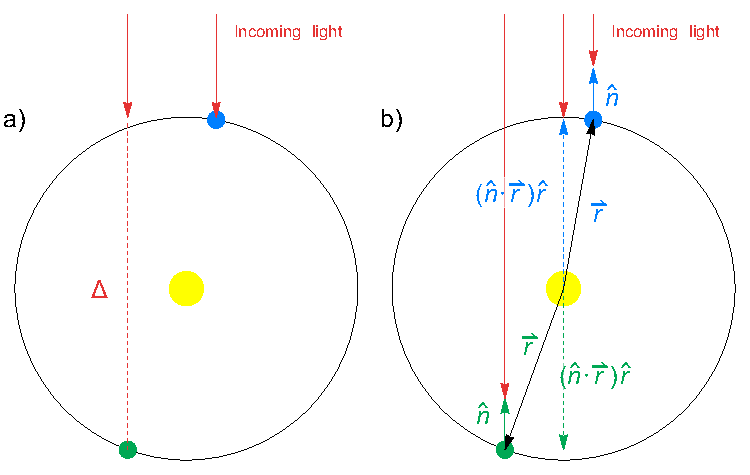
\includegraphics[width=0.9\textwidth]{img/Heliocentric.pdf}
	%\captionsetup{width=\textwidth}
	\caption[Conceptual view of the R\o{}mer delay]{ Conceptual view of the R\o{}mer delay for a signal coming from above (in red). 
	The comparison is made between the earth at two points of its orbit (blue and green disks) around the sun (yellow disk).
	\textbf{a)} The distance $\Delta$ that the incoming light has to travel if the earth is in the opposite side of its orbit (green earth) will mean a time delay of $\Delta/c$
	relative to the nearest part of the orbit (blue earth).
	The limit value for $\Delta$ is $\sim2$ AU, so the time delay would be around $16$ minutes.
	\textbf{b)} This time the excess distance is calculated from the sun, and its value is the projection of the sun-to-earth vector to the vector normal to the incoming signal.
	}
	\label{fig:romer-delay}
\end{figure}


\begin{figure}
	\centering
	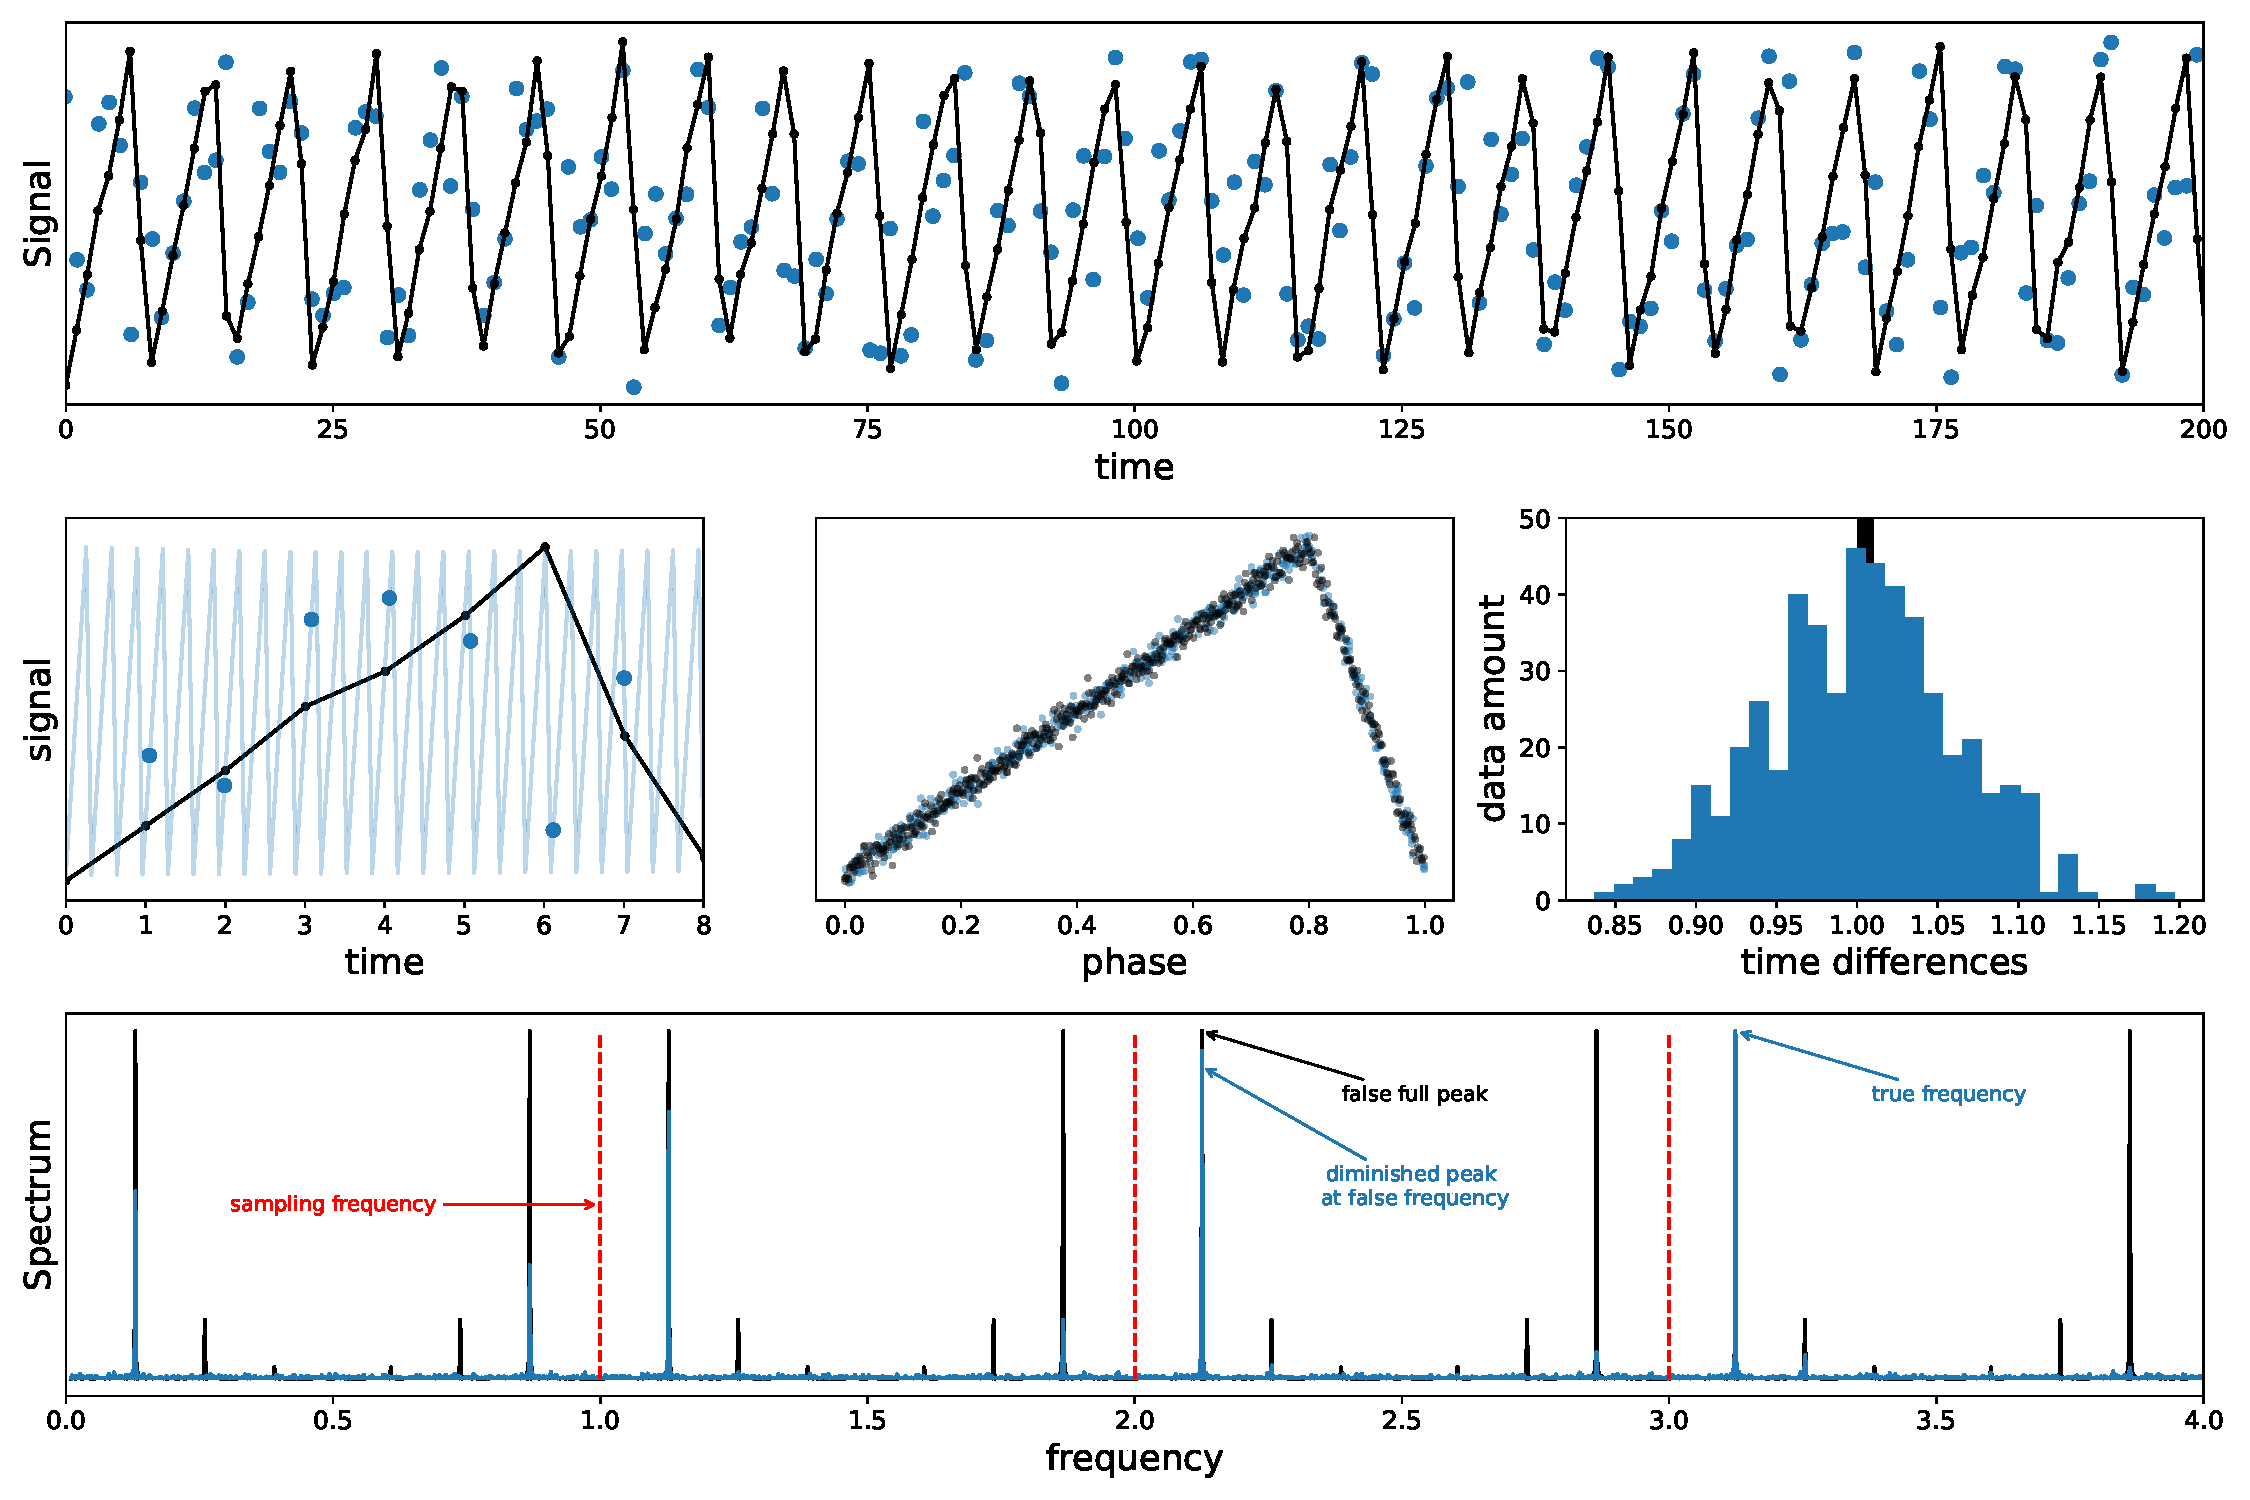
\includegraphics[width=\textwidth]{img/uneven_advantage.pdf}
	\caption[Comparison between even and uneven sampled signal past the nyquist limit]{
		Sample skewed triangular wave sampled two ways: the black dots are sampled one each unit of time.
		The sample times of the blue dots are very near one sample each unit of time, but have a litte dispersion,
		as can be seen in the left histogram.
		The frequency of the generated data is 3.124 time units.
		It is clear that the spectrum reflects every half of the sampling time (Nyquist frequency). 
		On the uneven sampling case, the spectrum does not reflect exactly; there are peaks greater than others,
		and the differences last until several times past the sampling frequency.
		The greatest peak is in the correct frequency, and the rest are partially canceled out.
		This cancellation auments with the dispersion on the sampling times, and the number of data.
		The detailed curve on the mid-left shows how exactly this happens: if the frequency is high, the dots with take an entire different path on the curve with the slightests of the temporal deviations.
	}
	\label{fig:uneven-advantage}
\end{figure}


\begin{figure}
	\centering
	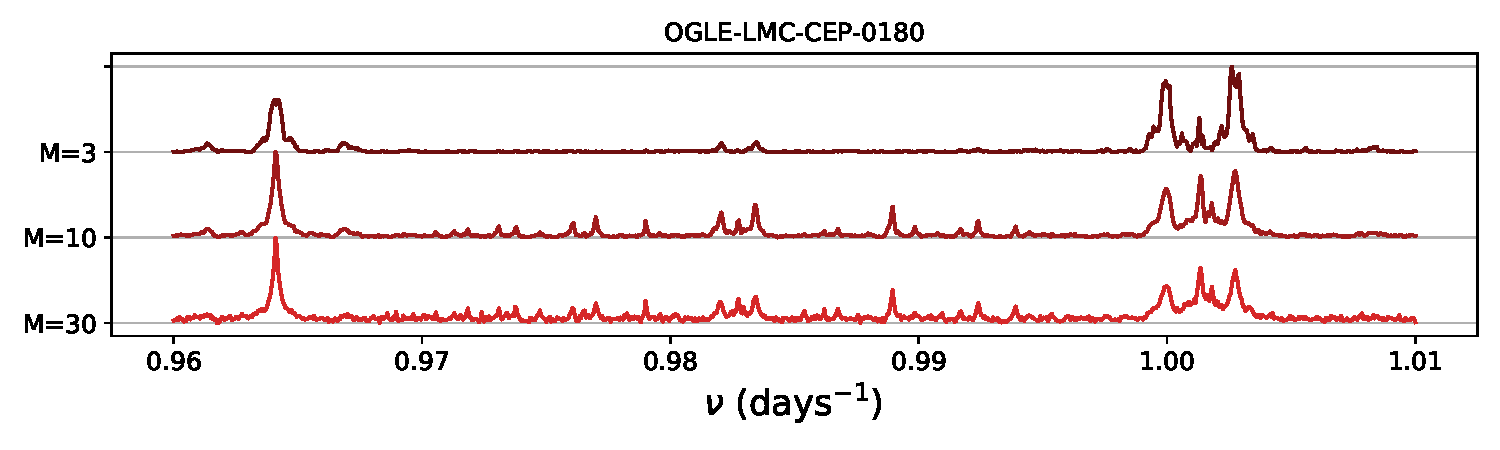
\includegraphics[width=\textwidth]{img/entropy_bins.pdf}
	\caption[Example of zone number dependency for the entropy method]{
		Entropy method applied to the same star over the same interval, but with varying number of zones per axis.
		The total number of zones would be $m=M^2$. 
		The first peak that can be observed at around $\nu=0.965$/day is the correct frequency for this star.
		The peaks near $\nu=1$/day are alias peaks, explained on \autoref{fig:problem}.
		The lower the number of zones, the higher the alias peaks compared to the true peak.
		At low number of zones there is also considerably less noise with respect to the fourier spectrum 
		(see \autoref{fig:examples} for a comparison), and the process of taking the entropy is faster.
		This compromise between speed, noise levels and false peak heights should be taken into account 
		for any application of the entropy periodogram, unless a way to eliminate the false peaks is found,
		as in the case of the Fourier, Lomb-Scargle and dispersion periodograms.
	}
	\label{fig:entropy-alias}
\end{figure}

\begin{figure}
	\centering
	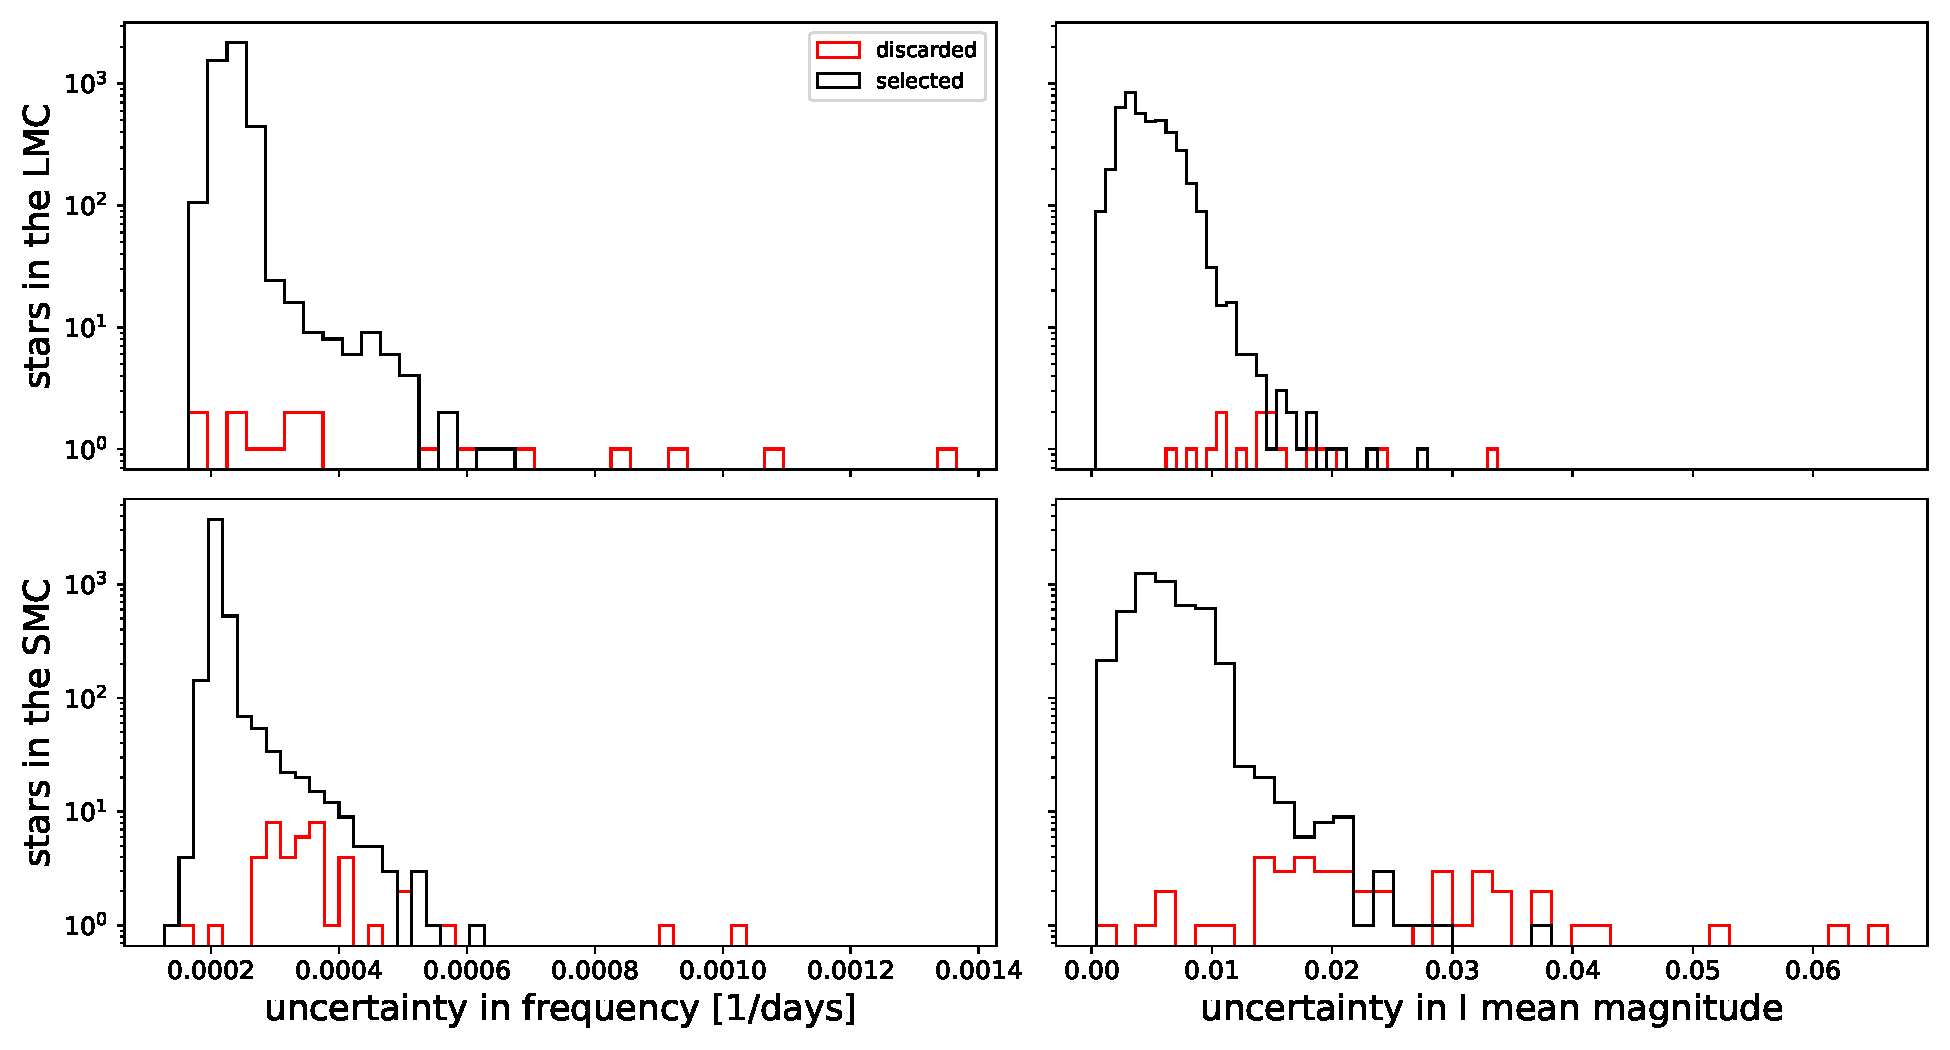
\includegraphics[width=\textwidth]{img/results_uncertainties.pdf}
	\caption[Uncertainties in the PL relation for the processed stars]{
		Distribution of uncertainties on calculations for the PL diagram, for the selected (black) and discarded (red) stars on each cloud, 
		according to the criteria discussed on \autoref{fig:peaks-n-points}.
		The uncertainty of the peaks are their full width at half maximum, 
		and the uncertainties in mean magnitude were calculated with a combination of pooled variance from each measurement and statistical bootstrap.
	}
	\label{fig:uncertainties}
\end{figure}


\begin{figure}
	\centering
	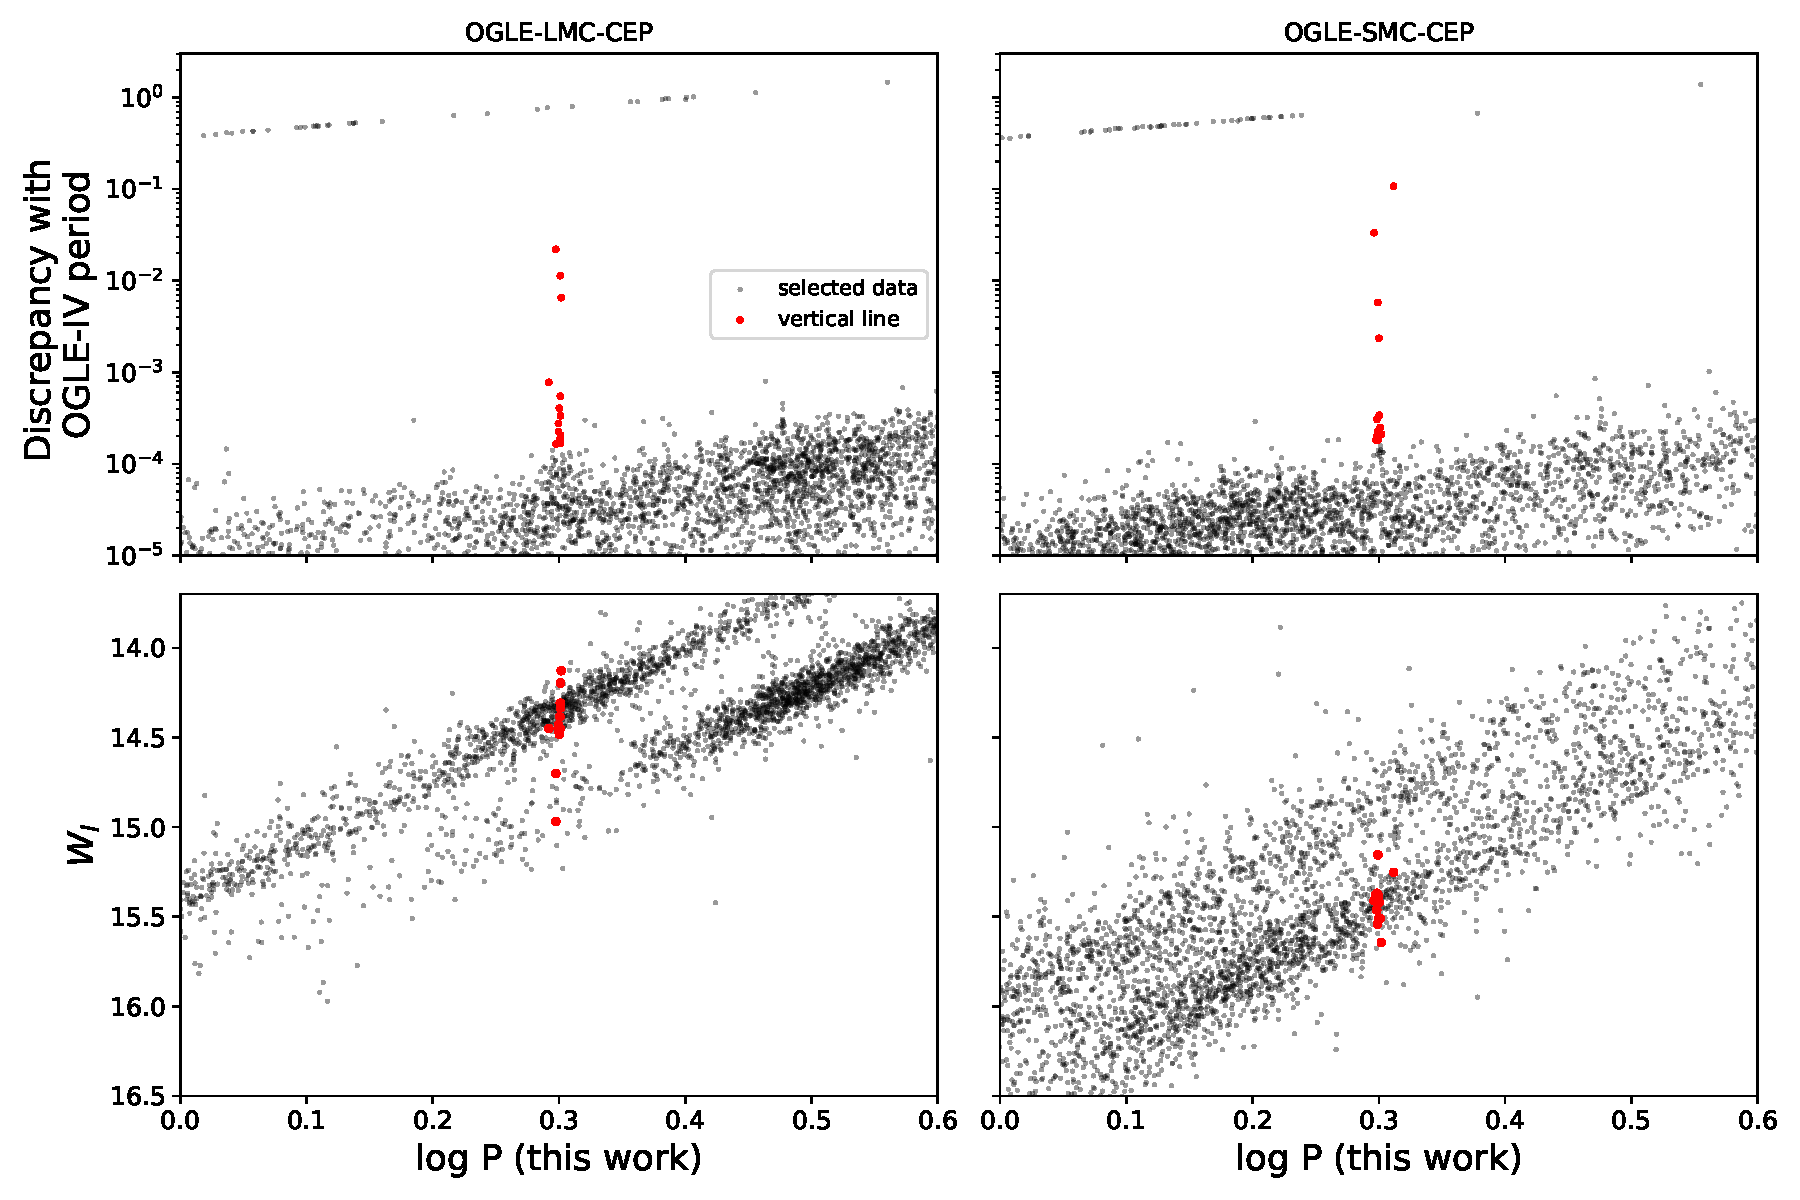
\includegraphics[width=\textwidth]{img/vertial_line_detail.pdf}
	\caption[Detail of the vertical line on the discrepancy plot]{
		Detail of the vertical bridge between the zones of low and high discrepancy of \autoref{fig:comparison}.
		The range used to capture the stars on this vertical line, shown in red, were $-3.8<\log \Delta P < -0.8$ and $0.28 < \log P < 0.32 $.
		In the SMC case, the line curves at the end, and seemengly continues alognside the horizontal line of high discrepancy.
	}
	\label{fig:vertical-discrepancy}
\end{figure}


\begin{figure}
	\centering
	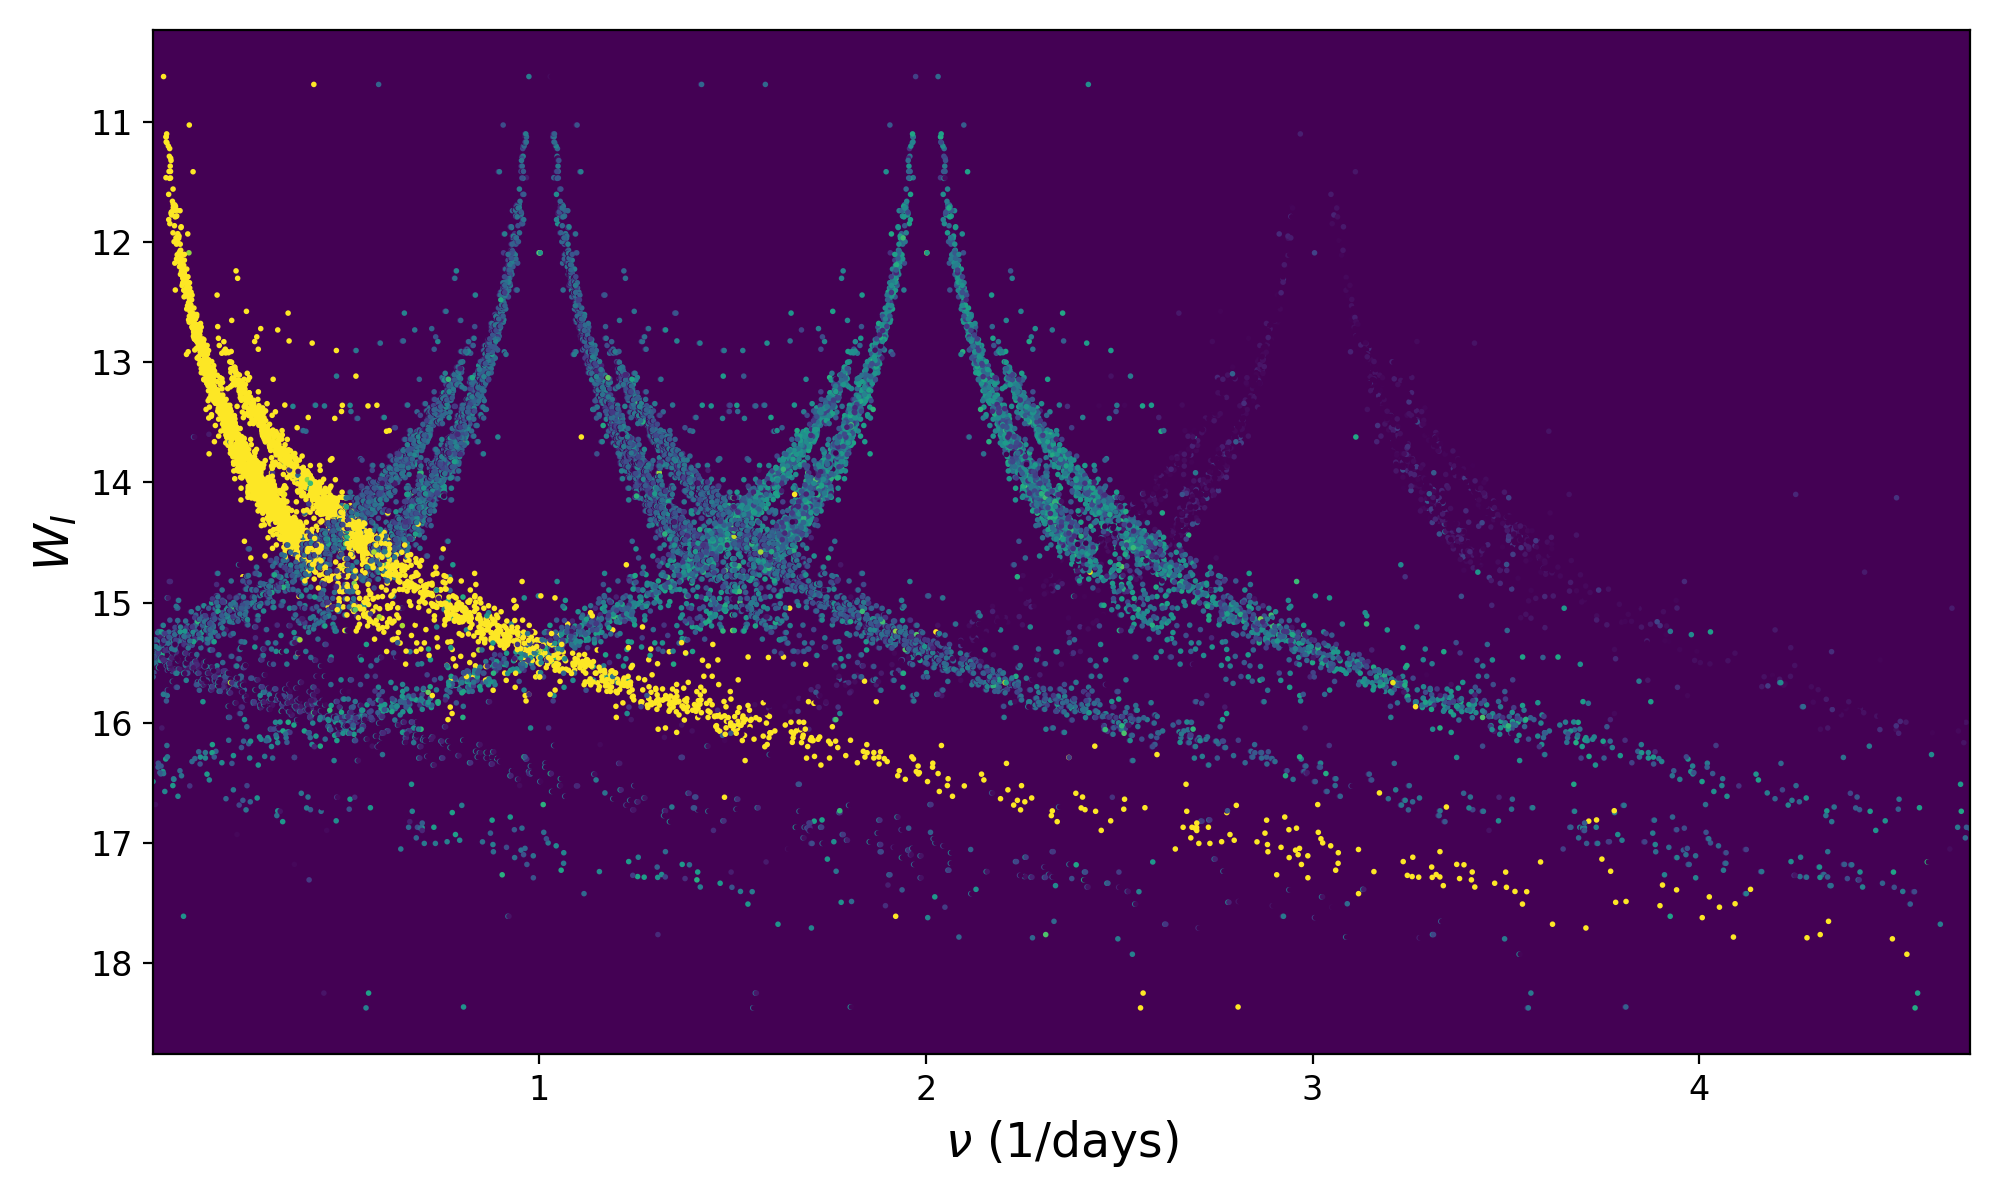
\includegraphics[width=\textwidth]{img/lmc_freq.png}
	\caption[Linear frequency PL relation with secondary peaks for the LMC]{
		PL diagram for the LMC, but the x-axis is the linear frequency grid where the periods were searched.
		Principal peaks are shown in yellow, and secondary in more bluer colors, according to their peak heights on the spectrogram.
		As the temporal cadence of the data is something around 1 day, the situation is a perfect realization of the example plots from \autoref{fig:uneven-advantage};
		the spectrograms reflect horizontally every 0.5/day, which is half the \enquote{mean} sampling frequency (modulo 1, see \autoref{fig:1234-cadence}) and 
		if it were not for the uneven sampling, all the less prominent peaks would be equal in height to the principal frequency peak.
		Effectively, for frequencies higher than 0.5 would be impossible to tell apart the true peaks from the alias ones.
	}
	\label{fig:linear-color-pl-lmc}
\end{figure}

\begin{figure}
	\centering
	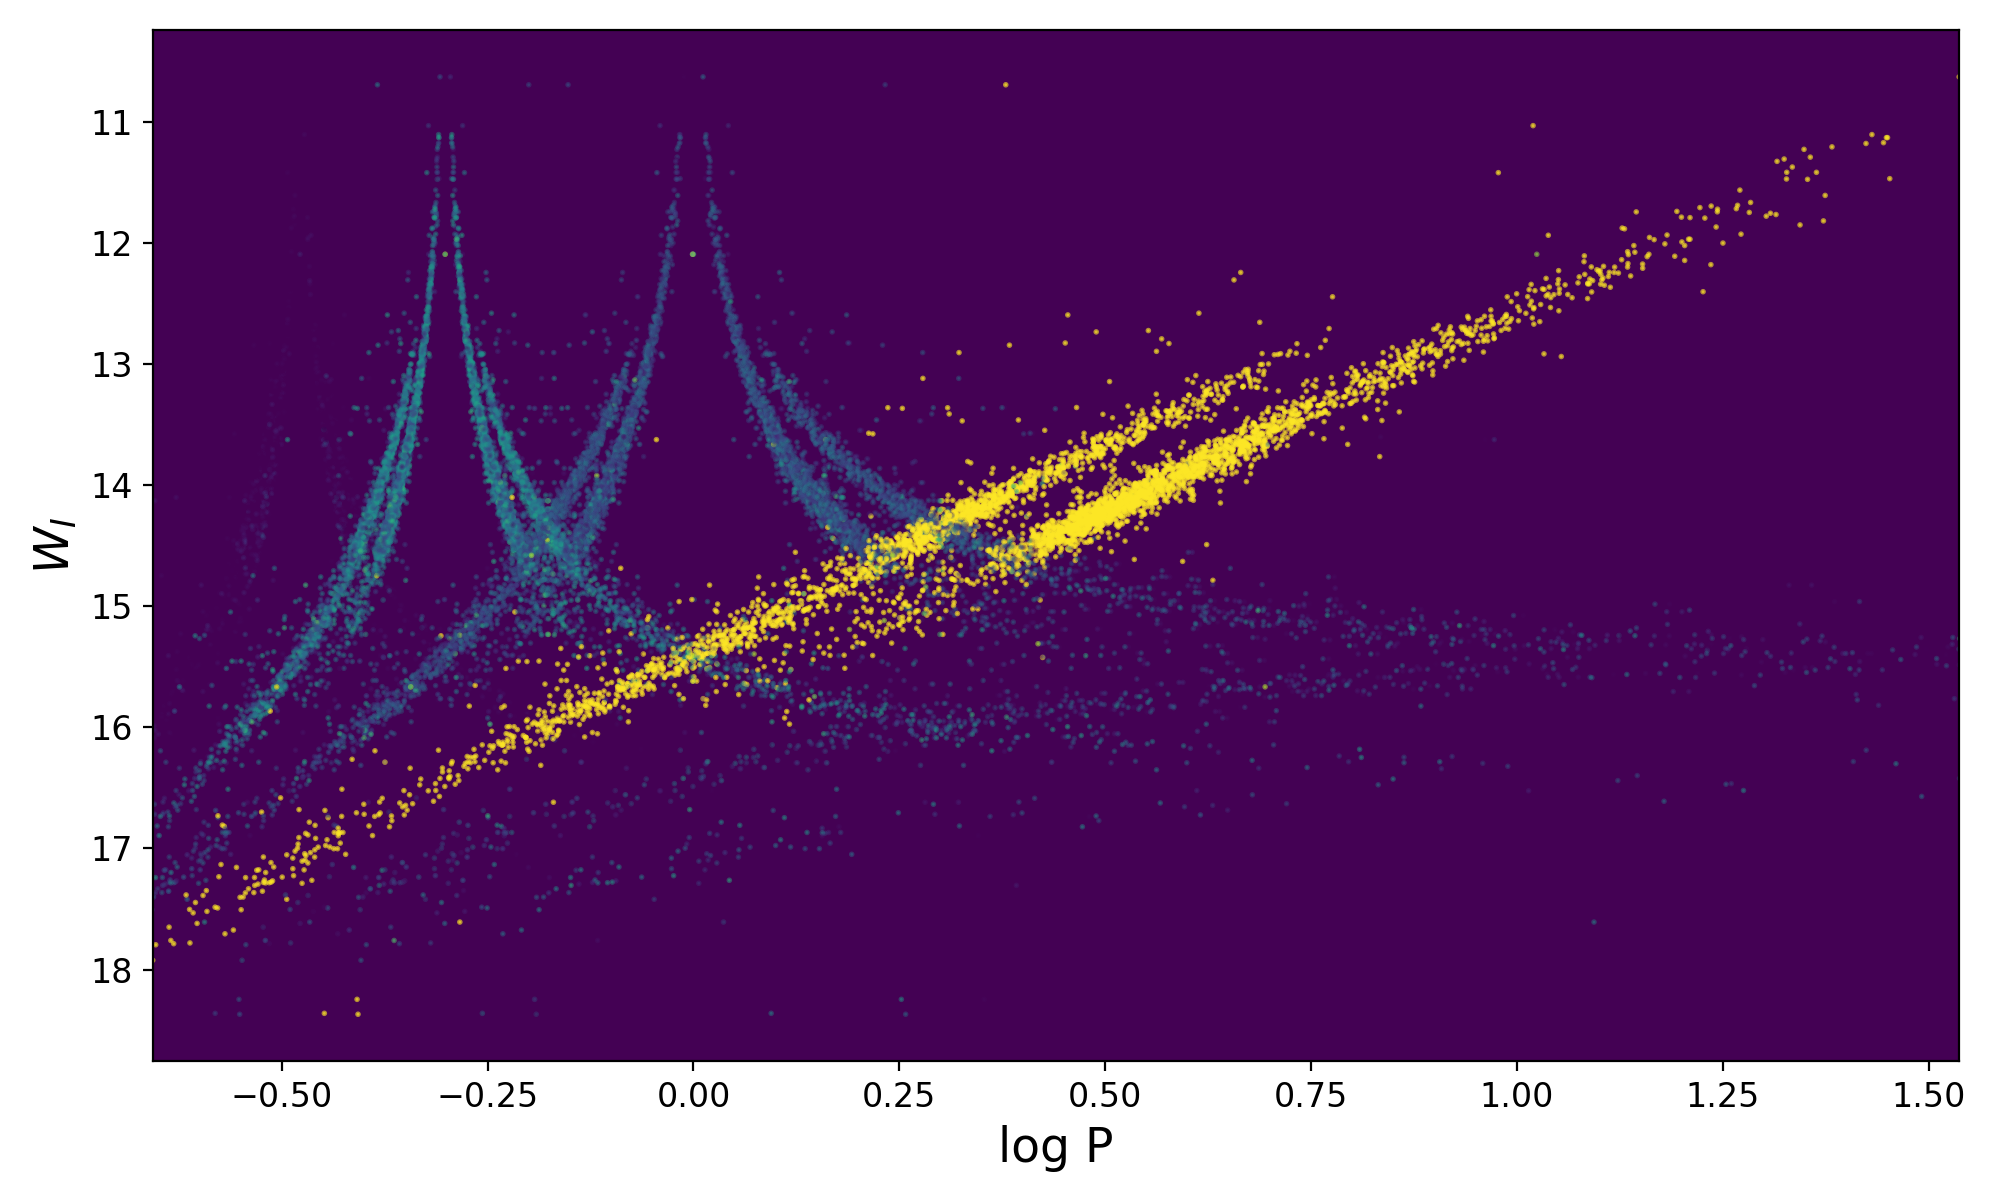
\includegraphics[width=\textwidth]{img/lmc.png}
	\caption[PL relation with secondary peaks for the LMC]{
		Period-Luminosity relation for the LMC, but showing all the peaks on the spectrum for each star above noise level. 
		The principal peak is shown in yellow, and subsequent peaks in bluer colors according to their relative heights.
		Each horizontal line of this graphic could be thought as an intensity image of the star Fourier spectrum.
	}
	\label{fig:color-pl-lmc}
\end{figure}


\begin{figure}
	\centering
	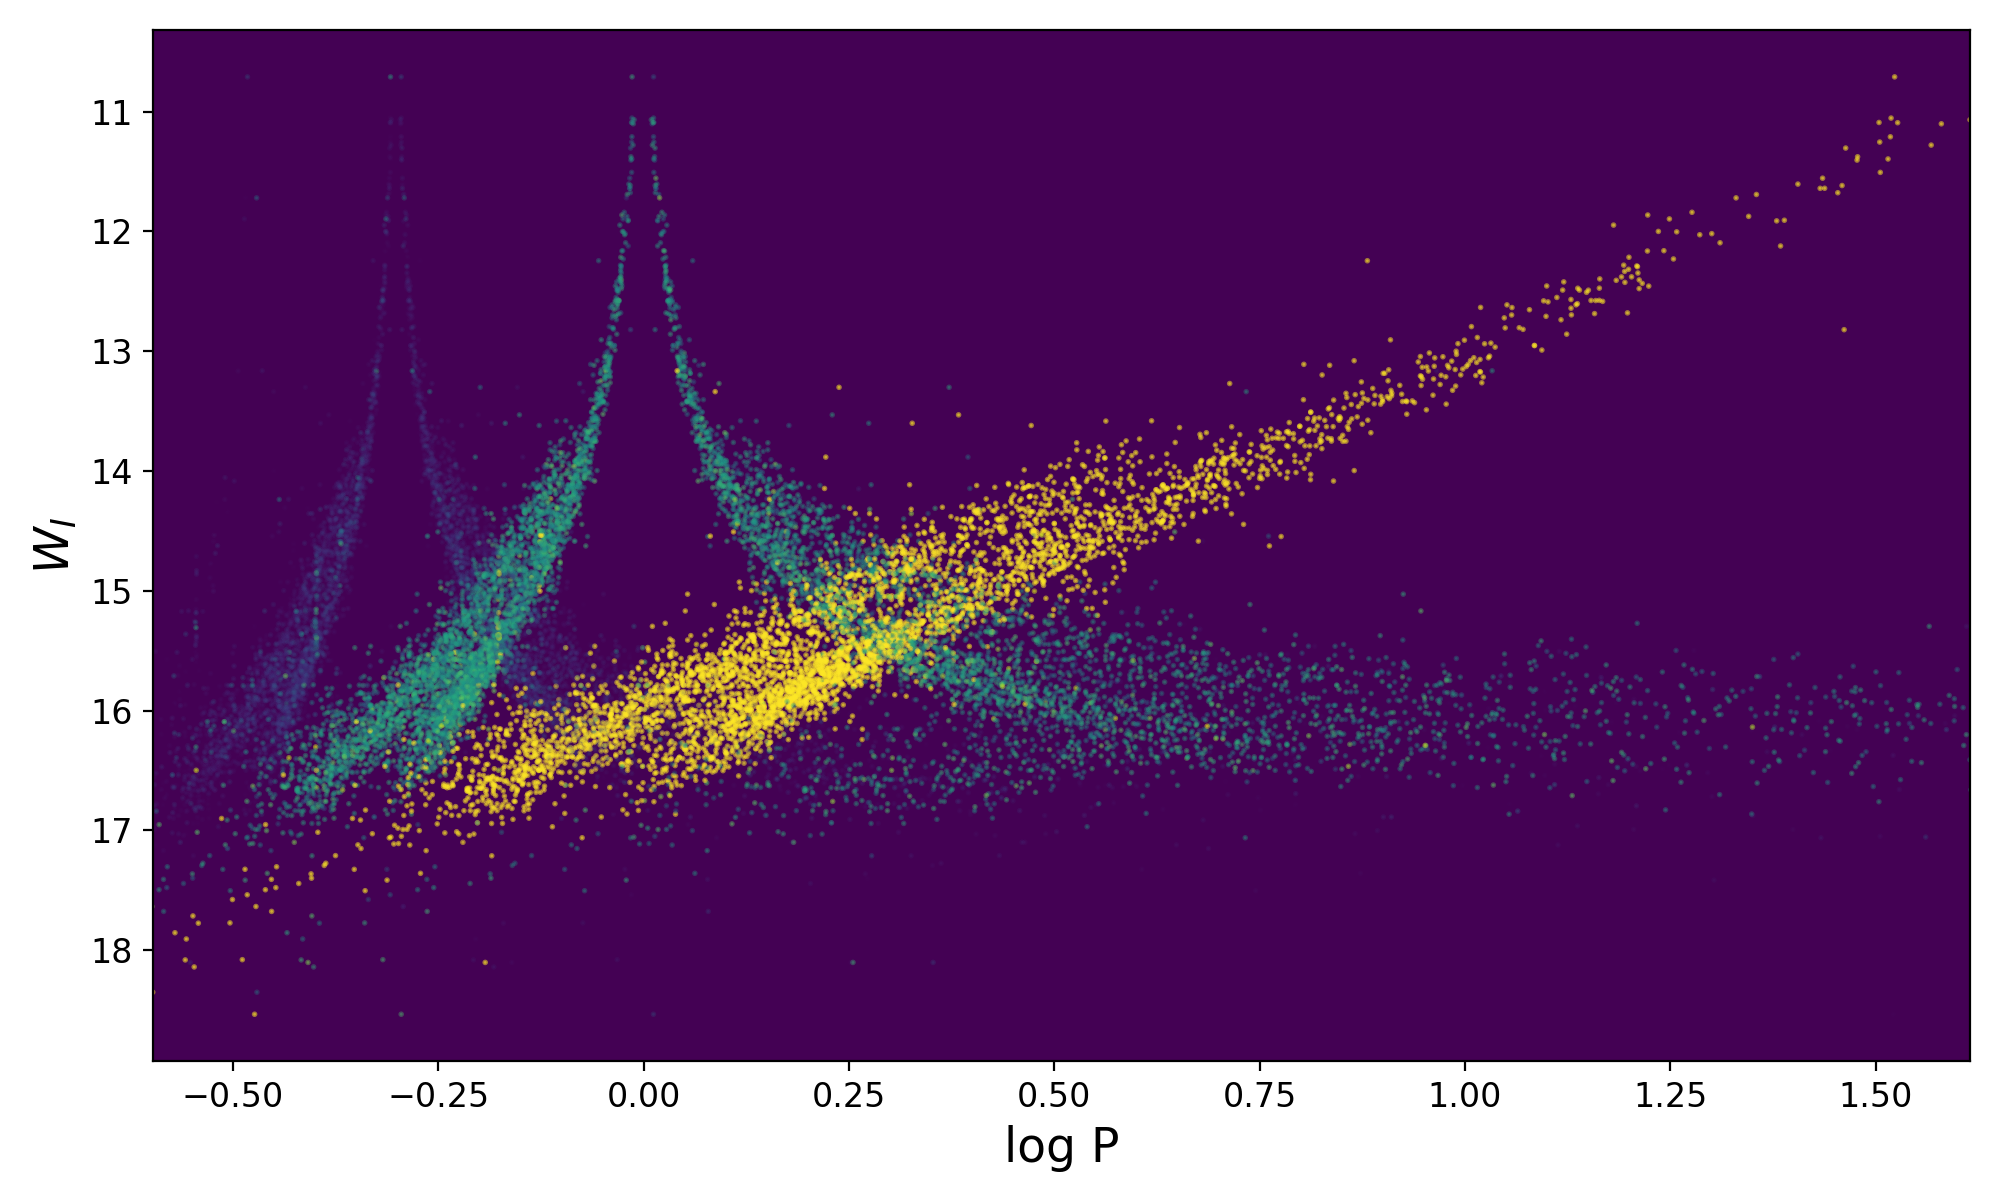
\includegraphics[width=\textwidth]{img/smc.png}
	\caption[PL relation with secondary peaks for the SMC]{
		Period-Luminosity relation for the SMC, but showing all the peaks on the spectrum for each star above noise level. 
		The principal peak is shown in yellow, and subsequent peaks in bluer colors according to their relative heights.
	}
	\label{fig:color-pl-smc}
\end{figure}







\end{document}

